%!TEX root = ../thesis.tex

\graphicspath{{assets/chapter_5/}}

\chapter{Channel Shaping using \glsfmtshort{ris}: From Diagonal Model to Beyond}\label{ch:channel_shaping}




\begin{section}{Introduction}
	% The quest for reliable, high-speed, and ubiquitous wireless connectivity has been long-standing since Marconi's illuminating radio in 1895.
	% Great successes have been made at transmitter and receiver sides over the past century, and the society is unprecedentedly close to the Shannon limit \cite{Shannon1948}.
	Today we are witnessing a paradigm shift from connectivity to intelligence, where the wireless environment is no longer a chaotic medium but a conscious agent that serves on demand.
	This is empowered by the recent advances in \gls{ris}, a real-time programmable metasurface of numerous non-resonant sub-wavelength scattering elements.
	It can manipulate the amplitude, phase, frequency, and polarization of the scattered waves \cite{Basar2019} with a higher energy efficiency, lower cost, lighter footprint, and greater scalability than relays.
	Using \gls{ris} for {passive beamforming} has attracted significant interest in wireless communication \cite{Wu2019,Wu2020c,Yang2020,Zheng2021}, backscatter \cite{Jia2020,Liang2022}, sensing \cite{Liu2022a,Hua2023}, and power transfer literature \cite{Wu2021d,Feng2022,Zhao2022}, reporting a second-order array gain and fourth-order power scaling law (with proper waveform).
	On the other hand, \gls{ris} also enables {backscatter modulation} by dynamically switching between different patterns, as already investigated \cite{Karasik2020,Basar2020,Zhao2022a} and prototyped \cite{Tang2019b,Dai2020a}.
	Despite fruitful outcomes, one critical unanswered question is the {channel shaping} capability: \emph{To what extent can a passive \gls{ris} reshape the wireless channel?}

	The answer depends heavily on the hardware architecture and scattering model.
	In diagonal \gls{ris}, each scattering element is tuned by a dedicated impedance and acts as an \emph{individual} phase shifter \cite{Wu2020}.
	The concept is generalized to \gls{bd}-\gls{ris} \cite{Shen2020a,Li2023b} which physically connects adjacent elements using passive components.
	This allows \emph{cooperative} scattering --- wave impinging on one element can propagate within the circuit and depart partially from any element in the same group.
	\gls{bd}-\gls{ris} can thus control both amplitude and phase of the reflected wave, generalizing the scattering matrix from diagonal with unit-magnitude entries \eqref{eq:diagonal_scattering_matrix} to block diagonal with unitary blocks \eqref{eq:bd_scattering_matrix}.
	Its benefit has been recently shown in receive power maximization \cite{Nerini2023,Santamaria2023,Fang2023,Nerini2024}, transmit power minimization \cite{Zhou2023}, and rate maximization \cite{Zhou2023,Nerini2024,Li2023d,Bartoli2023,Li2023c}.
	Practical issues such as channel estimation \cite{Li2023e} and mutual coupling \cite{Li2023f} have also been investigated.
	Therefore, \gls{bd}-\gls{ris} is envisioned as the next generation channel shaper with stronger signal processing flexibility \cite{Li2023g}.

	% Attempts to characterize the channel shaping capability can be classified into \emph{singular value centric} and \emph{power centric} methods.
	% Channel shaping is different from passive beamforming as it seeks to modify the inherent properties of the channel itself, allowing one to decouple \gls{ris} and transceiver design.
	Channel shaping is different from passive beamforming discussed in Chapters \ref{ch:ris_aided_swipt} and \ref{ch:riscatter} because \gls{ris} is exploited as a stand-alone device to modify the inherent properties of the wireless channel.
	This allows one to decouple the \gls{ris}-transceiver design and explore the fundamental limits of wave manipulation.
	Relevant design criteria can be roughly classified into two categories:
	\begin{itemize}
		\item \emph{Singular value centric:} Focus on the singular values of the equivalent channel matrix, which are closely related to the channel capacity and the diversity-multiplexing trade-off. Relevant designs are more complicated since they involve the entire channel matrix.
		\item \emph{Power centric:} Focus on the second-order characteristics of the channel matrix, which are useful in \gls{miso} but less informative in \gls{mimo}. Relevant designs are more practical and straightforward.
	\end{itemize}
	The former has been studied in terms of minimum singular value \cite{ElMossallamy2021}, effective rank \cite{ElMossallamy2021,Meng2023}, condition number \cite{Zheng2022,Huang2023} in \gls{pc}, and degree of freedom \cite{Bafghi2022,Zheng2023,Chae2023} in \gls{ic}.
	The latter has been studied in terms of channel power \cite{Wu2019,Nerini2023,Santamaria2023} in \gls{pc} and leakage interference \cite{Santamaria2023a} in \gls{ic}.
	Although the results are insightful, the big picture is far from complete since there exists neither a systematic channel shaping study nor a universal \gls{ris} optimization framework.
	To the best of our knowledge, the most general channel shaping scenario (\gls{bd}-\gls{ris}-aided \gls{mimo}) has not been studied, and the great potential of \gls{bd}-\gls{ris} has not been fully exploited or understood.
	This chapter aims for a comprehensive answer to the channel shaping question through theoretical analysis and numerical optimization.
	The contributions are summarized below.

	First, we exploit the Riemannian geometry of the Stiefel manifold to design a novel geodesic\footnote{A geodesic refers to the shortest path between two points in a Riemannian manifold.} \gls{rcg} algorithm for \gls{bd}-\gls{ris} optimization.
	This method modified from \cite{Abrudan2008,Abrudan2009} not only features lower complexity and faster convergence than general non-geodesic approach \cite{Absil2009,Pan2022d}, but also fits arbitrary group size and any smooth \gls{ris} optimization problem.
	Specifically, block-wise rotational update is performed along the geodesics of the Stiefel manifold, which are expressed compactly by the exponential map \cite{Edelman1998}.
	This is the first work to tailor an efficient optimization framework for asymmetric \gls{bd}-\gls{ris}.

	Second, we quantify the capability of a \gls{bd}-\gls{ris} to redistribute the singular values of \gls{mimo}-\gls{pc}.
	The \emph{Pareto frontiers} are characterized by optimizing the {weighted sum of singular values}, where the weights can be positive, zero, or negative.
	This problem is solved by the proposed geodesic \gls{rcg} algorithm.
	The resulting achievable singular value region generalizes most relevant metrics and provides an intuitive channel shaping benchmark.
	We also demystify the \gls{bd}-\gls{ris} gain from off-diagonal entries and derive some analytical singular value bounds for rank-deficient \gls{mimo} and fully-connected (a.k.a. unitary) \gls{ris}.
	This is the first work to comprehensively answer the channel shaping question and fully unveil the potential or \gls{bd}-\gls{ris}.

	Third, we tackle \gls{bd}-\gls{ris}-aided \gls{mimo}-\gls{pc} rate maximization with two solutions: a local-optimal approach through \gls{ao} and a low-complexity approach over channel shaping.
	The former updates active and passive beamforming by eigenmode transmission and \gls{rcg} algorithm, respectively.
	The latter suboptimally decouples both blocks, recasts the shaping problem as channel power maximization, and solves it iteratively in closed form.
	Interestingly, the gap in between vanishes as \gls{bd}-\gls{ris} evolves from diagonal to unitary.
	It suggests channel shaping decouples the \gls{ris}-transceiver design and offers a promising low-complexity solution.
	This is the first work to discuss the implications of channel shaping in joint active-passive beamforming optimization.

	Fourth, we extend the aforementioned approaches to \gls{mimo}-\gls{ic} where the \gls{bd}-\gls{ris} is used for leakage interference minimization and \gls{wsr} maximization.
	In the former case, we update the receive combiner, transmit precoder, and scattering matrix iteratively in closed forms with optimality proof.
	In the latter case, we alternatively updates the transmit precoder by bisection and the scattering matrix by \gls{rcg} algorithm.
	We also compare the impact of \gls{ris} on \gls{pc} and \gls{ic}.
	% provide a comprehensive comparison between the two approaches and discuss the implications of channel shaping in \gls{ic}.



	% Fifth, extensive simulations reveal that the performance gain from \gls{bd}-\gls{ris} increases with group size and \gls{mimo} dimensions.
	% In terms of channel power, fully-connected \gls{bd}-\gls{ris} boosts up to 62\% and 270\% over diagonal \gls{ris} in $1 \times 1$ and $4 \times 4$ \gls{mimo} under independent Rayleigh fading, respectively.
	% The superiority stems from stronger \emph{subchannel rearrangement} and \emph{subspace alignment} capabilities empowered by in-group cooperation.
	% It emphasizes the importance of using \gls{bd}-\gls{ris} in large-scale \gls{mimo} systems.


\end{section}


\begin{section}{\glsfmtshort{mimo}-\glsfmtshort{pc}}
	\begin{subsection}{System Model}
		Consider a \gls{bd}-\gls{ris}-aided point-to-point \gls{mimo} system with $N_\mathrm{T}$, $N_\mathrm{S}$, $N_\mathrm{R}$ transmit, scatter, and receive antennas, respectively.
		This configuration is denoted as $N_\mathrm{T} \times N_\mathrm{S} \times N_\mathrm{R}$ in the following context.
		The \gls{bd}-\gls{ris} can be modeled as an $N_\mathrm{S}$-port network \cite{Ivrlac2010} that divides into $G$ individual groups, each containing $L \triangleq N_\mathrm{S} / G$ elements interconnected by real-time reconfigurable components \cite{Shen2020a}.
		To simplify the analysis, we assume a lossless asymmetric network\footnote{While symmetric \gls{bd}-\gls{ris} (involving capacitors and inductors) is often considered in the literature \cite{Shen2020a,Nerini2023,Santamaria2023,Fang2023,Nerini2024,Zhou2023,Li2023d,Bartoli2023}, asymmetric \gls{bd}-\gls{ris} can be built over reconfigurable asymmetric passive components (e.g., ring hybrids and branch-line hybrids) \cite{Ahn2006}.} without mutual coupling between scatter elements, as previously considered in \cite{Li2023b,Li2023c,Bartoli2023}.
		The overall scattering matrix of the \gls{bd}-\gls{ris} is
		\begin{equation}
			\mathbf{\Theta} = \mathrm{diag}(\mathbf{\Theta}_1,\ldots,\mathbf{\Theta}_G),
		\end{equation}
		where $\mathbf{\Theta}_g \in \mathbb{U}^{L \times L}$ is a unitary matrix that describes the response of group $g \in \mathcal{G} \triangleq \{1, \ldots, G\}$.
		That is, $\mathbf{\Theta}_g^\mathsf{H} \mathbf{\Theta}_g = \mathbf{I}$.
		Note that diagonal (single-connected) and unitary (fully-connected) \gls{ris} can be regarded as its extreme cases with group size $L=1$ and $L=N_\mathrm{S}$, respectively.
		Some potential physical architectures of \gls{bd}-\gls{ris} are illustrated in \cite[Fig. 3]{Shen2020a}, \cite[Fig. 5]{Li2023c}, and \cite[Fig. 2]{Nerini2024}, where the radiation pattern and circuit topology have impacts on the scattering matrix.

		Let $\mathbf{H}_\mathrm{D} \in \mathbb{C}^{N_\mathrm{R} \times N_\mathrm{T}}$, $\mathbf{H}_\mathrm{B} \in \mathbb{C}^{N_\mathrm{R} \times N_\mathrm{S}}$, $\mathbf{H}_\mathrm{F} \in \mathbb{C}^{N_\mathrm{S} \times N_\mathrm{T}}$ denote the direct (transmitter-receiver), backward (\gls{ris}-receiver), and forward (transmitter-\gls{ris}) channels, respectively.
		The equivalent channel is a function of the scattering matrix
		\begin{equation}
			\mathbf{H} = \mathbf{H}_\mathrm{D} + \mathbf{H}_\mathrm{B} \mathbf{\Theta} \mathbf{H}_\mathrm{F} = \mathbf{H}_\mathrm{D} + \sum_g \mathbf{H}_{\mathrm{B},g} \mathbf{\Theta}_g \mathbf{H}_{\mathrm{F},g},
			\label{eq:channel_equivalent}
		\end{equation}
		where $\mathbf{H}_{\mathrm{B},g} \in \mathbb{C}^{N_\mathrm{R} \times L}$ and $\mathbf{H}_{\mathrm{F},g} \in \mathbb{C}^{L \times N_\mathrm{T}}$ are the backward and forward subchannels for \gls{ris} group $g$, corresponding to the $(g-1)L$ to $gL$ columns of $\mathbf{H}_\mathrm{B}$ and rows of $\mathbf{H}_\mathrm{F}$, respectively.
		% That is, $\mathbf{H}_{\mathrm{B},g}$ (resp. $\mathbf{H}_{\mathrm{F},g}$) corresponds to the $(g-1)L$ to $gL$ columns (resp. rows) of $\mathbf{H}_\mathrm{B}$ (resp. $\mathbf{H}_\mathrm{F}$).
		% , corresponding to the $(g-1)L$ to $gL$ columns of $\mathbf{H}_\mathrm{B}$ and rows of $\mathbf{H}_\mathrm{F}$.
		% $\mathbf{H}_{\mathrm{B},g}$ (resp. $\mathbf{H}_{\mathrm{F},g}$) corresponds to the $(g-1)L$ to $gL$ columns of $\mathbf{H}_\mathrm{B}$
		Since unitary matrices constitute an algebraic group with respect to multiplication, the scattering matrix of group $g$ can be decomposed as
		\begin{equation}
			\mathbf{\Theta}_g = \mathbf{L}_g \mathbf{R}_g^\mathsf{H},
			\label{eq:unitary_decomposition}
		\end{equation}
		where $\mathbf{L}_g, \mathbf{R}_g \in \mathbb{U}^{L \times L}$ are two unitary factor matrices.
		Let $\mathbf{H}_{\mathrm{B},g} = \mathbf{U}_{\mathrm{B},g} \mathbf{\Sigma}_{\mathrm{B},g} \mathbf{V}_{\mathrm{B},g}^\mathsf{H}$ and $\mathbf{H}_{\mathrm{F},g} = \mathbf{U}_{\mathrm{F},g} \mathbf{\Sigma}_{\mathrm{F},g} \mathbf{V}_{\mathrm{F},g}^\mathsf{H}$ be the compact \gls{svd} of the backward and forward channels, respectively.
		The equivalent channel can thus be rewritten as
		\begin{equation}
			\mathbf{H} = \overbrace{\mathbf{H}_\mathrm{D} + \sum_g \mathbf{U}_{\mathrm{B},g} \mathbf{\Sigma}_{\mathrm{B},g} \underbrace{\mathbf{V}_{\mathrm{B},g}^\mathsf{H} \mathbf{L}_g \mathbf{R}_g^\mathsf{H} \mathbf{U}_{\mathrm{F},g}}_\text{backward-forward} \mathbf{\Sigma}_{\mathrm{F},g} \mathbf{V}_{\mathrm{F},g}^\mathsf{H}}^\text{direct-indirect}.
			\label{eq:channel_equivalent_svd}
		\end{equation}

		\begin{remark}\label{rm:channel_shaping}
			By analyzing \eqref{eq:channel_equivalent_svd}, we conclude that channel shaping through \gls{bd}-\gls{ris} creates two critical opportunities:
			\begin{itemize}
				\item \textbf{Subspace alignment:} Each group can align the singular matrices of the backward-forward (intra-group, multiplicative) and the direct-indirect (inter-group, additive) channels. In \gls{siso}, subspace alignment boils down to phase matching and the optimal scattering matrix of group $g$ is
				\begin{equation}
					\mathbf{\Theta}_g^\star = \exp \bigl(\jmath \mathrm{arg}(h_\mathrm{D})\bigr) \mathbf{V}_{\mathrm{B},g} \mathbf{U}_{\mathrm{F},g}^\mathsf{H},
				\end{equation}
				where $\mathbf{V}_{\mathrm{B},g} = \bigl[\mathbf{h}_{\mathrm{B},g}/\lVert \mathbf{h}_{\mathrm{B},g} \rVert, \mathbf{N}_{\mathrm{B},g}\bigr]$, $\mathbf{U}_{\mathrm{F},g} = \bigl[\mathbf{h}_{\mathrm{F},g}/\lVert \mathbf{h}_{\mathrm{F},g} \rVert, \mathbf{N}_{\mathrm{F},g}\bigr]$, and $\mathbf{N}_{\mathrm{B},g}, \mathbf{N}_{\mathrm{F},g} \in \mathbb{C}^{L \times (L-1)}$ are the orthonormal bases of the null spaces of $\mathbf{h}_{\mathrm{B},g}$ and $\mathbf{h}_{\mathrm{F},g}$, respectively.
				Diagonal \gls{ris} is thus sufficient for perfect \gls{siso} phase matching (with empty null spaces), but its disadvantage in subspace alignment scales with \gls{mimo} dimensions, since each element can only apply a common phase shift to the ``pinhole'' indirect channel of size $N_\mathrm{R} \times N_\mathrm{T}$ passing through itself.
				Even if the \gls{bd}-\gls{ris} is fully-connected, there still exists a trade-off between the direct-indirect and backward-forward alignments.
				\item \textbf{Subchannel rearrangement:} This unique property of \gls{bd}-\gls{ris} allows each group to rearrange and combine the backward and forward subchannels by strength. In \gls{siso}, diagonal \gls{ris} provides a maximum indirect channel amplitude of $\sum_{n=1}^{N_\mathrm{S}} \lvert h_{\mathrm{B},n} \rvert \lvert h_{\mathrm{F},n} \rvert$, while \gls{bd}-\gls{ris} can generalize it to $\sum_{g=1}^{G} \sum_{l=1}^{L} \lvert h_{\mathrm{B},\pi_{\mathrm{B},g}(l)} \rvert \lvert h_{\mathrm{F},\pi_{\mathrm{F},g}(l)} \rvert$, where $\pi_{\mathrm{B},g}$ and $\pi_{\mathrm{F},g}$ are permutations of $\mathcal{L} \triangleq \{1, \ldots, L\}$. By rearrangement inequality, the maximum is attained by pairing the $l$-th strongest backward and forward subchannels in each group.
				The advantage of \gls{bd}-\gls{ris} in subchannel rearrangement scales with \gls{mimo} dimensions, since the number of subchannels associated with each group grows with $N_\mathrm{R} \times N_\mathrm{T}$.
			\end{itemize}
		\end{remark}

		% TODO: add illustrations for both

		% In \gls{siso}, the equivalent channel can be further simplified as
		% \begin{equation}
		% 	h = h_\mathrm{D} + \sum_g \mathbf{h}_{\mathrm{B},g} \mathbf{\Theta}_g \mathbf{h}_{\mathrm{F},g},
		% \end{equation}
		% subspace alignment boils down to phase matching




		% For the \gls{siso} case in Fig. \subref*{fg:power_bond_txrx1_nd}, the maximum channel power is approximately \num{4e-6} by diagonal \gls{ris} and \num{6.5e-6} by fully-connected \gls{bd}-\gls{ris}, corresponding to a \qty{62.5}{\percent} gain.
		% This aligns with the asymptotic \gls{bd}-\gls{ris} scaling law derived for \gls{siso} in \cite{Shen2020a}.
		% Interestingly, the gain surges to \qty{270}{\percent} in 4T4R \gls{mimo} as shown in Fig. \subref*{fg:power_bond_txrx4_nd}.
		% This is because subspace alignment boils down to phase matching in \gls{siso} such that both triangular and Cauchy-Schwarz inequalities in \cite[(50)]{Shen2020a} can be simultaneously tight regardless of the group size.
		% That is, diagonal \gls{ris} is sufficient for subspace alignment in \gls{siso} while the \qty{62.5}{\percent} gain from \gls{bd}-\gls{ris} comes purely from subchannel rearrangement (i.e., pairing the forward and backward channels from strongest to weakest).
		% Now consider a diagonal \gls{ris} in \gls{mimo}.
		% Each element can only apply a common phase shift to the associated rank-1 $N_\mathrm{R} \times N_\mathrm{T}$ indirect channel.
		% Therefore, perfect subspace alignment of indirect channels through different elements is generally impossible.
		% It means the disadvantage of diagonal \gls{ris} in subspace alignment and subchannel rearrangement scales with \gls{mimo} dimensions.
		% We thus conclude that the power gain of \gls{bd}-\gls{ris} scales with group size and \gls{mimo} dimensions.


		% \begin{equation}
		% 	\mathbf{H} = \underbrace{\mathbf{H}_\mathrm{D} + \underbrace{\sum_g \mathbf{U}_{\mathrm{B},g} \mathbf{\Sigma}_{\mathrm{B},g} \underbrace{\mathbf{V}_{\mathrm{B},g}^\mathsf{H} \mathbf{L}_g \mathbf{R}_g^\mathsf{H} \mathbf{U}_{\mathrm{F},g}}_\text{backward-forward} \mathbf{\Sigma}_{\mathrm{F},g} \mathbf{V}_{\mathrm{F},g}^\mathsf{H}}_\text{group-wise}}_\text{direct-indirect},
		% \end{equation}
		% which involves three subspace alignment problems:
		% which involves three subspace alignment problems
		% \begin{equation}
		% 	\mathbf{H} = \mathbf{H}_\mathrm{D} + \sum_g \mathbf{U}_{\mathrm{B},g} \mathbf{\Sigma}_{\mathrm{B},g} \underbrace{\mathbf{V}_{\mathrm{B},g}^\mathsf{H} \mathbf{L}_g \mathbf{R}_g^\mathsf{H} \mathbf{U}_{\mathrm{F},g}}_{\substack{\text{backward-forward}\\\text{additive alignment}}} \mathbf{\Sigma}_{\mathrm{F},g} \mathbf{V}_{\mathrm{F},g}^\mathsf{H}.
		% \end{equation}
		% \begin{equation}
		% 	\mathbf{H} = \mathbf{H}_\mathrm{D} + \sum_g \mathbf{U}_{\mathrm{B},g} \mathbf{\Sigma}_{\mathrm{B},g} \underbrace{\mathbf{V}_{\mathrm{B},g}^\mathsf{H} \mathbf{L}_g}_{\substack{\text{backward}\\\text{align}}} \underbrace{\mathbf{R}_g^\mathsf{H} \mathbf{U}_{\mathrm{F},g}}_{\substack{\text{forward}\\\text{align}}} \mathbf{\Sigma}_{\mathrm{F},g} \mathbf{V}_{\mathrm{F},g}^\mathsf{H}.
		% \end{equation}
		% Then the equivalent channel can be rewritten as
		% Since the field of (block) unitary matrices formulate a field that is closed under multiplication
		% Since block unitary matrices satisfy the axioms of a field under matrix multiplication
		% \begin{remark}
		% 	% To understand the \gls{b} gain from in-group connections
		% \end{remark}




		% \begin{remark}
		% 	From \eqref{eq:scattering_fc} and \eqref{eq:channel_equivalent_fc} in the proof of Proposition \ref{pp:fully_connected}, we notice that \eqref{iq:sv_bound_fc}--\eqref{iq:sv_bound_fc_power} are simultaneously tight when
		% 	% Interestingly, \eqref{iq:sv_bound_fc}--\eqref{iq:sv_bound_fc_power} are simultaneously tight when
		% 	\begin{equation}
		% 		\mathbf{\Theta} = \mathbf{V}_\mathrm{B} \mathbf{U}_\mathrm{F}^\mathsf{H}.
		% 		\label{eq:scattering_fc_tight}
		% 	\end{equation}
		% 	An interpretation is that the off-diagonal entries can enhance the capabilities of
		% 	\begin{itemize}
		% 		\item subspace alignment: $\mathbf{V}_\mathrm{B}$ and $\mathbf{U}_\mathrm{F}^\mathsf{H}$ in \eqref{eq:scattering_fc} fully align the subspaces of $\mathbf{H}_\mathrm{B}$ and $\mathbf{H}_\mathrm{F}$ by rotation;
		% 		\item subchannel rearrangement: $\mathbf{X} = \mathbf{I}$ in \eqref{eq:channel_equivalent_fc} pairs the subchannels of $\mathbf{H}_\mathrm{B}$ and $\mathbf{H}_\mathrm{F}$ from strongest to weakest, which attains the maximum in rearrangement inequality.
		% 	\end{itemize}
		% \end{remark}



		% \begin{remark}
		% 	\gls{bd}-\gls{ris} reduces to diagonal \gls{ris} and unitary \gls{ris} with group size $L$ 1 and $N_\mathrm{S}$, respectively.
		% \end{remark}
		% \begin{remark}
		% 	Individual forward and backward \gls{csi} are required for \gls{bd}-\gls{ris} designs.
		% 	This is different from diagonal \gls{ris} where estimating their product is usually sufficient.
		% 	% Later we will show the potential benefits from the \gls{csi} overhead.
		% \end{remark}
	\end{subsection}


	\begin{subsection}{Channel Singular Values Redistribution}
		\begin{subsubsection}{A Toy Example}\label{sc:toy_example}
			We first illustrate the channel shaping capabilities of different \gls{ris} by a toy example.
			% We first use a toy example to illustrate that \gls{bd}-\gls{ris} can provide a wider dynamic range of channel singular values.
			Consider a $2 \times 2 \times 2$ setup where the direct link is blocked.
			The diagonal \gls{ris} is modeled by $\mathbf{\Theta}_\mathrm{D} = \mathrm{diag}(e^{\jmath \theta_1}, e^{\jmath \theta_2})$ while the unitary \gls{bd}-\gls{ris} has 4 independent angular parameters
			\begin{equation}
				\mathbf{\Theta}_\mathrm{U} = e^{\jmath \phi} \begin{bmatrix}
					e^{\jmath \alpha} \cos \psi  & e^{\jmath \beta} \sin \psi   \\
					-e^{-\jmath \beta} \sin \psi & e^{-\jmath \alpha} \cos \psi
				\end{bmatrix}.
			\end{equation}
			It is worth noting that $\phi$ has no impact on the singular value because $\mathrm{sv}(e^{\jmath \phi} \mathbf{A}) = \mathrm{sv}(\mathbf{A})$.
			For a fair comparison, we also enforce symmetry $\mathbf{\Theta}_\mathrm{U} = \mathbf{\Theta}_\mathrm{U}^\mathsf{T}$ by $\beta = \pi / 2$ such that both architectures have the same number of angular parameters.
			\begin{figure}
				\centering
				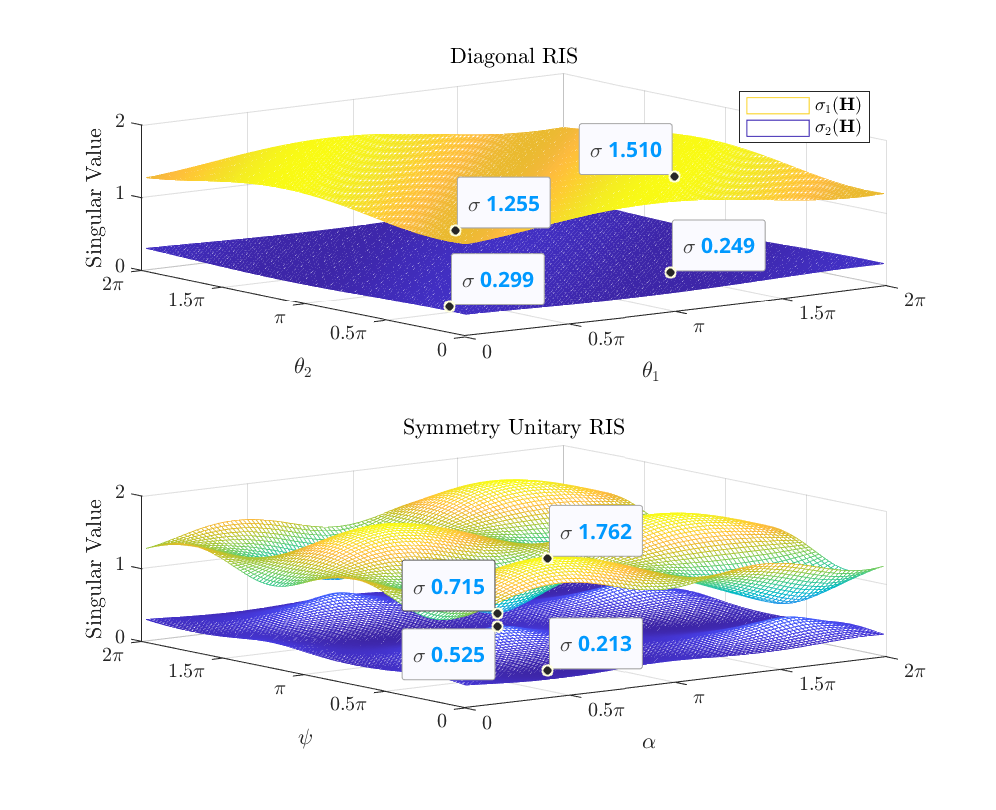
\includegraphics[width=\columnwidth]{assets/chapter_5/singular_trend.eps}
				\caption{$2 \times 2 \times 2$ (no direct) channel singular value shaping by diagonal and symmetry unitary \gls{ris}.}
				\label{fg:singular_trend}
			\end{figure}
			Fig.~\ref{fg:singular_trend} shows the channel singular values achieved by an exhaustive grid search over $(\theta_1, \theta_2)$ for diagonal \gls{ris} and $(\alpha, \psi)$ for symmetric unitary \gls{ris}.
			It is observed that both singular values can be manipulated up to $9\%$ using diagonal \gls{ris} and $42\%$ using symmetric \gls{bd}-\gls{ris}, despite both architectures have the same number of scattering elements and design parameters.
			A larger performance gap is expected when asymmetric \gls{bd}-\gls{ris} is available.
			This example shows \gls{bd}-\gls{ris} can provide a wider dynamic range of channel singular values and motivates further studies on channel shaping.
		\end{subsubsection}

		\begin{subsubsection}{Pareto Frontier Characterization}\label{sc:pareto_frontier}
			We then characterize the Pareto frontier of channel singular values by maximizing their weighted sum
			\begin{maxi!}
				{\scriptstyle{\mathbf{\Theta}}}{\sum_n \rho_n \sigma_n(\mathbf{H})}{\label{op:pareto}}{\label{ob:pareto}}
				\addConstraint{\mathbf{\Theta}_g^\mathsf{H} \mathbf{\Theta}_g=\mathbf{I},}{\quad \forall g,}{\label{co:pareto_unitary}}
			\end{maxi!}
			where $n \in \{1,\ldots,N \triangleq \min(N_\mathrm{T}, N_\mathrm{R})\}$ and $\rho_n$ is the weight of the $n$-th singular value that can be positive, zero, or negative.
			Varying $\{\rho_n\}$ unveils the entire achievable singular value region.
			Thus, we claim the Pareto frontier problem~\eqref{op:pareto} generalizes most relevant metrics and provides a powerful shaping framework.
			The objective \eqref{ob:pareto} is smooth in $\mathbf{\Theta}$ and the feasible domain \eqref{co:pareto_unitary} for group $g$ corresponds to the Stiefel manifold.
			Next, we zoom out and provide an efficient optimization framework for asymmetric \gls{bd}-\gls{ris}.

			Inspired by \cite{Abrudan2008,Abrudan2009}, we propose a block-wise \gls{rcg} algorithm along the geodesics on the Lie group of unitary matrices $\mathbb{U}^{L \times L}$.
			It leverages the fact that unitary matrices are closed under multiplication.
			At iteration $r$, the gradient is computed in the Euclidean space and translated to the Riemannian manifold \cite{Absil2009}
			\begin{gather}
				\nabla_{\mathrm{E},g}^{(r)} = \frac{\partial f(\mathbf{\Theta}_g^{(r)})}{\partial \mathbf{\Theta}_g^*},\label{eq:gradient_euclidean}\\
				\nabla_{\mathrm{R},g}^{(r)} = \nabla_{\mathrm{E},g}^{(r)} {\mathbf{\Theta}_g^{(r)}}^\mathsf{H} - \mathbf{\Theta}_g^{(r)} {\nabla_{\mathrm{E},g}^{(r)}}^\mathsf{H}.\label{eq:gradient_riemannian} % $\mathcal{O}(N_\mathrm{S}^3)$
			\end{gather}
			The Polak-Ribierre parameter \cite{Polak1969} is approximated as \cite{Abrudan2009}
			\begin{equation}
				\gamma_g^{(r)} = \frac{\mathrm{tr}\bigl((\nabla_{\mathrm{R},g}^{(r)} - \nabla_{\mathrm{R},g}^{(r-1)}) {\nabla_{\mathrm{R},g}^{(r)}}^\mathsf{H}\bigr)}{\mathrm{tr}\bigl(\nabla_{\mathrm{R},g}^{(r-1)} {\nabla_{\mathrm{R},g}^{(r-1)}}^\mathsf{H}\bigr)}, % $\mathcal{O}(2 N_\mathrm{S}^3 + N_\mathrm{S}^2 + 2 N_\mathrm{S})$
				\label{eq:parameter_cg}
			\end{equation}
			and the conjugate direction is
			\begin{equation}
				\mathbf{D}_g^{(r)} = \nabla_{\mathrm{R},g}^{(r)} + \gamma_g^{(r)} \mathbf{D}_g^{(r-1)}. % $\mathcal{O}(N_\mathrm{S}^2)$
				\label{eq:direction_cg}
			\end{equation}
			In the Stiefel manifold, the geodesic emanating from $\mathbf{\Theta}_g^{(r)}$ with velocity $\mathbf{D}_g^{(r)}$ and step size $\mu$ is described compactly by the exponential map \cite{Edelman1998}
			\begin{equation}
				\mathbf{G}_g^{(r)}(\mu) = \exp(\mu \mathbf{D}_g^{(r)}) \mathbf{\Theta}_g^{(r)}. % $\mathcal{O}(N_\mathrm{S}^3)$
				\label{eq:geodesic}
			\end{equation}
			An appropriate $\mu^\star$ can be obtained by the Armijo rule \cite{Armijo1966}.
			To double the step size, one can simply square the rotation matrix instead of recomputing the matrix exponential, i.e., $\exp(2 \mu \mathbf{D}_g^{(r)}) = \exp^2(\mu \mathbf{D}_g^{(r)})$.
			To halve the step size, taking its square root is sufficient in theory but is subject to numerical instability in practice.
			Finally, the scattering matrix is updated along the geodesic as
			\begin{equation}
				\mathbf{\Theta}_g^{(r+1)} = \mathbf{G}_g^{(r)}(\mu^\star).
				\label{eq:update_geodesic}
			\end{equation}
			Algorithm~\ref{ag:rcg} summarizes the proposed block-wise geodesic \gls{rcg} method for smooth maximization problems of asymmetric \gls{bd}-\gls{ris}.
			Convergence to stationary points is guaranteed.

			\begin{remark}
				Compared with universal manifold optimization \cite{Absil2009,Pan2022d}, Algorithm~\ref{ag:rcg} inherits a trifold benefit from \cite{Abrudan2008,Abrudan2009}:
				\begin{enumerate}
					\item No retraction from Euclidean space to Stiefel manifold thanks to rotational update \eqref{eq:geodesic}, \eqref{eq:update_geodesic};
					\item Lower computational complexity per iteration;
					\item Faster convergence thanks to proper parameter space.
				\end{enumerate}
			\end{remark}

			% \setalgorithmcaptionfont{\small}
			\begin{algorithm}[!t]
				% \small
				\caption{Block-wise geodesic \gls{rcg} for asymmetric \gls{bd}-\gls{ris}}
				\label{ag:rcg}
				\begin{algorithmic}[1]
					\Require $f(\mathbf{\Theta})$, $G$
					\Ensure $\mathbf{\Theta}^\star$
					\Initialize {$r \gets 0$, $\mathbf{\Theta}^{(0)}$}
					\Repeat
						\For {$g \gets 1$ to $G$}
							\State $\nabla_{\mathrm{E},g}^{(r)} \gets$ \eqref{eq:gradient_euclidean} \label{ln:gradient_euclidean}
							\State $\nabla_{\mathrm{R},g}^{(r)} \gets$ \eqref{eq:gradient_riemannian}
							\State $\gamma_g^{(r)} \gets$ \eqref{eq:parameter_cg}
							\State $\mathbf{D}_g^{(r)} \gets$ \eqref{eq:direction_cg}
							\If {$\Re\bigl\{\mathrm{tr}({\mathbf{D}_g^{(r)}}^\mathsf{H} \nabla_{\mathrm{R},g}^{(r)})\bigr\} < 0$} \Comment{not an ascent direction}
								\State $\mathbf{D}_g^{(r)} \gets \nabla_{\mathrm{R},g}^{(r)}$
							\EndIf
							\State $\mu \gets 1$
							\State $\mathbf{G}_g^{(r)}(\mu) \gets$ \eqref{eq:geodesic}
							\While {$f\bigl(\mathbf{G}_g^{(r)}(2\mu)\bigr) - f(\mathbf{\Theta}_g^{(r)}) \ge \mu \cdot \mathrm{tr}(\mathbf{D}_g^{(r)} {\mathbf{D}_g^{(r)}}^\mathsf{H}) / 2$}
								\State $\mu \gets 2 \mu$
							\EndWhile
							\While {$f\bigl(\mathbf{G}_g^{(r)}(\mu)\bigr) - f(\mathbf{\Theta}_g^{(r)}) < \mu / 2 \cdot \mathrm{tr}(\mathbf{D}_g^{(r)} {\mathbf{D}_g^{(r)}}^\mathsf{H}) / 2$}
								\State $\mu \gets \mu / 2$
							\EndWhile
							\State $\mathbf{\Theta}_g^{(r+1)} \gets$ \eqref{eq:update_geodesic}
						\EndFor
						\State $r \gets r+1$
					\Until $\lvert f(\mathbf{\Theta}^{(r)}) - f(\mathbf{\Theta}^{(r-1)}) \rvert / f(\mathbf{\Theta}^{(r-1)}) \le \epsilon$
				\end{algorithmic}
			\end{algorithm}

			\begin{lemma}\label{lm:pareto_gradient}
				The Euclidean gradient of \eqref{ob:pareto} with respect to \gls{bd}-\gls{ris} group $g$ is
				\begin{equation}
					\frac{\partial \sum_n \rho_n \sigma_n(\mathbf{H})}{\partial \mathbf{\Theta}_g^*} = \mathbf{H}_{\mathrm{B},g}^\mathsf{H} \mathbf{U} \mathrm{diag}(\rho_1,\ldots,\rho_N) \mathbf{V}^\mathsf{H} \mathbf{H}_{\mathrm{F},g}^\mathsf{H},
					\label{eq:pareto_gradient}
				\end{equation}
				where $\mathbf{U}$ and $\mathbf{V}$ are the left and right singular matrices of $\mathbf{H}$, respectively.
			\end{lemma}
			\begin{proof}
				Please refer to Appendix~\ref{ap:pareto_gradient}.
			\end{proof}

			%  The Euclidean gradient of \gls{bd}-\gls{ris} group $g$ is computed as
			% where $\mathbf{U} \in \mathbb{C}^{N_\mathrm{R} \times N}$ and $\mathbf{V} \in \mathbb{C}^{N_\mathrm{T} \times N}$ are the left and right compact singular matrices of $\mathbf{H}$, respectively.
			Algorithm~\ref{ag:rcg} can thus be invoked for the Pareto singular value problem \eqref{op:pareto} where line \ref{ln:gradient_euclidean} uses \eqref{eq:pareto_gradient} explicitly.
			% \eqref{eq:pareto_gradient} is used in line \ref{ln:gradient_euclidean}.
		\end{subsubsection}

		\begin{subsubsection}{Some Analytical Bounds}\label{sc:bounds}
			We then discuss some interesting analytical bounds related to channel singular values.
			\begin{proposition}[Degree of freedom]\label{pp:dof}
				In point-to-point \gls{mimo}, \gls{bd}-\gls{ris} cannot achieve a higher \gls{dof} than diagonal \gls{ris}.
			\end{proposition}
			\begin{proof}
				Please refer to Appendix~\ref{ap:dof}.
			\end{proof}

			\begin{proposition}[Rank-deficient channel]\label{pp:rank_deficient}
				% If the forward/backward channel is rank-$k$, then a \gls{bd}-\gls{ris} can at most enlarge the $n$-th ($n > k$) channel singular value to the $n-k$-th singular value of $\mathbf{T}$, or suppress the $n$-th ($n < N - k + 1$) channel singular value to the $n$-th singular value of $\mathbf{T}$.
				% If the forward/backward channel is rank-$k$, then a sufficiently large \gls{bd}-\gls{ris} can at most enlarge (resp. suppress) the first (resp. last) $k$ equivalent channel singular values without bounds.
				If the forward or backward channel is rank-$k$, then regardless of the \gls{ris} size and architecture, the $n$-th singular value of the equivalent channel is bounded by
				\begin{align}
					\sigma_n(\mathbf{H}) & \le \sigma_{n-k}(\mathbf{T}), &  & \text{if } n > k, \label{iq:sv_bound_enlarge}          \\
					\sigma_n(\mathbf{H}) & \ge \sigma_n(\mathbf{T}),     &  & \text{if } n < N - k + 1, \label{iq:sv_bound_suppress}
				\end{align}
				where
				% \begin{align}
				% 	\mathbf{T} \mathbf{T}^\mathsf{H} = \mathbf{H}_\mathrm{D} (\mathbf{I} - \mathbf{V}_\mathrm{F} \mathbf{V}_\mathrm{F}^\mathsf{H}) \mathbf{H}_\mathrm{D}^\mathsf{H}, & \text{if } \mathrm{rank}(\mathbf{H}_\mathrm{F}) = k, \\
				% 	\mathbf{T}^\mathsf{H} \mathbf{T} = \mathbf{H}_\mathrm{D}^\mathsf{H} (\mathbf{I} - \mathbf{U}_\mathrm{F} \mathbf{U}_\mathrm{F}^\mathsf{H}) \mathbf{H}_\mathrm{D}, & \text{if } \mathrm{rank}(\mathbf{H}_\mathrm{B}) = k.
				% \end{align}
				\begin{equation}
					\mathbf{T} \mathbf{T}^\mathsf{H} =
					\begin{cases}
						\mathbf{H}_\mathrm{D} (\mathbf{I} - \mathbf{V}_\mathrm{F} \mathbf{V}_\mathrm{F}^\mathsf{H}) \mathbf{H}_\mathrm{D}^\mathsf{H}, & \text{if } \mathrm{rank}(\mathbf{H}_\mathrm{F}) = k, \\
						\mathbf{H}_\mathrm{D}^\mathsf{H} (\mathbf{I} - \mathbf{U}_\mathrm{B} \mathbf{U}_\mathrm{B}^\mathsf{H}) \mathbf{H}_\mathrm{D}, & \text{if } \mathrm{rank}(\mathbf{H}_\mathrm{B}) = k,
					\end{cases}
					\label{eq:auxiliary_matrix}
				\end{equation}
				and $\mathbf{V}_\mathrm{F}$ and $\mathbf{U}_\mathrm{B}$ are the right and left compact singular matrices of $\mathbf{H}_\mathrm{F}$ and $\mathbf{H}_\mathrm{B}$, respectively.
				% where $\mathbf{T} \mathbf{T}^\mathsf{H} = \mathbf{H}_\mathrm{D} (\mathbf{I} - \mathbf{V}_\mathrm{F} \mathbf{V}_\mathrm{F}^\mathsf{H}) \mathbf{H}_\mathrm{D}$ if the forward channel is rank-$k$ and $\mathbf{T}^\mathsf{H} \mathbf{T} = \mathbf{H}_\mathrm{D} (\mathbf{I} - \mathbf{U}_\mathrm{F} \mathbf{U}_\mathrm{F}^\mathsf{H}) \mathbf{H}_\mathrm{D}$ if the backward channel is rank-$k$.
			\end{proposition}
			\begin{proof}
				Please refer to Appendix~\ref{ap:rank_deficient}.
			\end{proof}

			% \begin{corollary}[degree of freedom]
			% 	In point-to-point \gls{mimo} with or without direct link, \gls{bd}-\gls{ris} cannot provide a higher \gls{dof} than diagonal \gls{ris}.
			% \end{corollary}

			\begin{corollary}[Extreme singular values\label{co:extreme}]
				With a sufficiently large \gls{ris}, the first $k$ channel singular values are unbounded above \footnote{\textellipsis while respecting energy conservation law $\sum_n \sigma_n^2 \le 1$. This constraint is omitted in the following context.} while the last $k$ channel singular values can be suppressed to zero.
				% For a rank-$k$ forward or backward channel with a sufficiently large \gls{ris}, the first $k$ singular values of the equivalent channel are unbounded above while the last $k$ singular values can be suppressed to zero.
				% If the forward or backward channel is rank-$k$ and the \gls{ris} is sufficiently large, then the first $k$ singular values of the equivalent channel are unbounded above while the last $k$ singular values can be suppressed to zero.
				% If the forward/backward channel is rank-$k$, then the first (resp. last) $k$ singular values of the equivalent channel are unbounded above (resp. below).
				% a sufficiently large \gls{ris} can at most enlarge (resp. suppress) the first (resp. last) $k$ singular values of the equivalent channel without bounds.
			\end{corollary}

			\begin{corollary}[\gls{los} channel\footnote{A similar result has been derived for diagonal \gls{ris} in \cite{Semmler2023}.}\label{co:los}]
				If the forward or backward channel is \gls{los}, then a \gls{ris} can at most enlarge (resp. suppress) the $n$-th ($n \ge 2$) channel singular value to the $(n-1)$-th (resp. $n$-th) singular value of $\mathbf{T}$, that is,
				\begin{equation}
					\sigma_1(\mathbf{H}) \ge \sigma_1(\mathbf{T}) \ge {\sigma_2(\mathbf{H})} \ge \ldots \ge \sigma_{N-1}(\mathbf{T}) \ge {\sigma_N(\mathbf{H})} \ge \sigma_N(\mathbf{T}).
					\label{iq:sv_bound_los}
				\end{equation}
			\end{corollary}

			In Section~\ref{sc:simulation}, we will show by simulation that a finite-size \gls{bd}-\gls{ris} can approach those bounds better than diagonal \gls{ris}.

			\begin{proposition}[Fully-connected \gls{ris} without direct link]\label{pp:fully_connected}
				% If the \gls{bd}-\gls{ris} is fully-connected and the direct link is absent, then the singular value bounds on $\mathbf{H}$ are equivalent to the singular value bounds on $\mathbf{BF}$, where $\mathbf{B}$ and $\mathbf{F}$ are arbitrary matrices with the same singular values as $\mathbf{H}_\mathrm{B}$ and $\mathbf{H}_\mathrm{F}$, respectively,
				If the \gls{bd}-\gls{ris} is fully-connected and the direct link is absent, then the channel singular values can be manipulated up to
				% If the \gls{bd}-\gls{ris} is fully-connected and the direct link is absent, then the bounds on the channel singular values are equivalent to the singular values of the equivalent channel, that is,
				% only bounds that apply here are those that apply to the singular values of
				\begin{equation}
					\mathrm{sv}(\mathbf{H}) = \mathrm{sv}(\mathbf{BF}),
				\end{equation}
				where $\mathbf{B}$ and $\mathbf{F}$ are arbitrary matrices with the same singular values as $\mathbf{H}_\mathrm{B}$ and $\mathbf{H}_\mathrm{F}$, respectively,
				% Our focus thus shifts to how the singular values of matrix product are bounded by the singular values of its individual factors.
			\end{proposition}

			\begin{proof}
				Please refer to Appendix~\ref{ap:fully_connected}.
			\end{proof}

			The problem now becomes \emph{how the singular values of matrix product are bounded by the singular values of its individual factors.}
			Let $N' = \max(N_\mathrm{T},N_\mathrm{S},N_\mathrm{R})$ and $\sigma_n(\mathbf{H})=\sigma_n(\mathbf{H}_\mathrm{F})=\sigma_n(\mathbf{H}_\mathrm{B})=0$ for $N < n \le N'$.
			We have the following corollaries.

			\begin{corollary}[Generic singular value bounds]
				\begin{equation}
					\prod_{k \in {K}} \sigma_k(\mathbf{H}) \le \prod_{i \in {I}} \sigma_i(\mathbf{H}_\mathrm{B}) \prod_{j \in {J}} \sigma_j(\mathbf{H}_\mathrm{F}),
					\label{iq:sv_bound_fc}
				\end{equation}
				for all admissible triples $(I, J, K) \in T_r^{N'}$ with $r < N'$, where
				\begin{equation*}
					\begin{gathered}
						% T_r^{N'} \triangleq \Bigl\{(I, J, K) \in U_r^{N'} \mid \text{for all } p < r \text{ and all } (F, G, H) \text{ in } T_p^r,\\
						% \sum_{f \in F} i_f + \sum_{g \in G} j_g \le \sum_{h \in H} k_h + p(p+1)/2 \Bigr\},
						T_r^{N'} \triangleq \Bigl\{(I, J, K) \in U_r^{N'} \mid \forall p < r, (F, G, H) \in T_p^r,\\
						\sum_{f \in F} i_f + \sum_{g \in G} j_g \le \sum_{h \in H} k_h + p(p+1)/2 \Bigr\},
					\end{gathered}
				\end{equation*}
				\begin{equation*}
					U_r^{N'} \triangleq \Bigl\{(I, J, K) \mid \sum_{i \in I} i + \sum_{j \in J} j = \sum_{k \in K} k + r(r+1)/2\Bigr\}.
				\end{equation*}
			\end{corollary}
			\begin{proof}
				Please refer to \cite[Theorem 8]{Fulton2000}. This implies the Corollaries~\ref{co:largest_singular_value} and \ref{co:product_singular_values}.
			\end{proof}

			\begin{corollary}[Upper bound on the largest singular value]\label{co:largest_singular_value}
				\begin{equation}
					\sigma_1(\mathbf{H}) \le \sigma_1(\mathbf{H}_\mathrm{B}) \sigma_1(\mathbf{H}_\mathrm{F}).
				\end{equation}
			\end{corollary}

			% \begin{corollary}[lower bound on the smallest singular value]
			% 	\begin{equation}
			% 		\sigma_{N'}(\mathbf{H}) \ge \sigma_{N'}(\mathbf{H}_\mathrm{B}) \sigma_{N'}(\mathbf{H}_\mathrm{F}).
			% 	\end{equation}
			% \end{corollary}

			\begin{corollary}[Upper bound on the product of first $k$ singular values]\label{co:product_singular_values}
				\begin{equation}
					\prod_{n=1}^k \sigma_n(\mathbf{H}) \le \prod_{n=1}^k \sigma_n(\mathbf{H}_\mathrm{B}) \prod_{n=1}^k \sigma_n(\mathbf{H}_\mathrm{F}).
				\end{equation}
			\end{corollary}

			% \begin{corollary}[lower bound on the product of last $k$ singular values]
			% 	\begin{equation}
			% 		\prod_{n=N'}^{N'-k+1} \sigma_n(\mathbf{H}) \ge \prod_{n=N'}^{N'-k+1} \sigma_n(\mathbf{H}_\mathrm{B}) \prod_{n=N'}^{N'-k+1} \sigma_n(\mathbf{H}_\mathrm{F}).
			% 	\end{equation}
			% \end{corollary}

			\begin{corollary}[Upper bound on the sum of first $k$ singular values to the power of $p$\label{co:sum_power}]
				\begin{equation}
					\sum_{n=1}^k \sigma_n^p(\mathbf{H}) \le \sum_{n=1}^k \sigma_n^p(\mathbf{H}_\mathrm{B}) \sigma_n^p(\mathbf{H}_\mathrm{F}), \quad p > 0.
					\label{iq:sv_bound_fc_power}
				\end{equation}
				When $k = N'$ and $p = 2$, \eqref{iq:sv_bound_fc_power} suggests the channel power is upper bounded by the sum of (sorted) element-wise power product of backward and forward subchannels.
			\end{corollary}
			\begin{proof}
				Please refer to \cite[Inequality 24.4.7]{Hogben2013}.
			\end{proof}

			\begin{remark}
				It is straightforward to verify \eqref{iq:sv_bound_fc}--\eqref{iq:sv_bound_fc_power} are simultaneously tight when
				\begin{equation}
					\mathbf{\Theta} = \mathbf{V}_\mathrm{B} \mathbf{U}_\mathrm{F}^\mathsf{H}.
					\label{eq:scattering_fc_tight}
				\end{equation}
				where $\mathbf{V}_\mathrm{B}$ and $\mathbf{U}_\mathrm{F}$ are the right and left compact singular matrices of $\mathbf{H}_\mathrm{B}$ and $\mathbf{H}_\mathrm{F}$, respectively.
			\end{remark}

			Tight bounds are inapplicable when a \gls{mimo} direct link is present, as the \gls{ris} needs to balance the direct-indirect (additive) and backward-forward (multiplicative) subspace alignments.
			Such a balance often involves optimization approaches discussed in Section~\ref{sc:pareto_frontier}. Another example will be discussed in Section~\ref{sc:low_complexity}.
		\end{subsubsection}

	\end{subsection}

	\begin{subsection}{Achievable Rate Maximization}\label{sc:rate}
		The \gls{mimo} achievable rate maximization problem can be formulated with respect to joint active and passive beamforming.
		This problem is different from channel shaping because the \gls{ris} is jointly design with the transmitter for an explicit objective
		\begin{maxi!}
			{\scriptstyle{\mathbf{W},\mathbf{\Theta}}}{R = \log \det \biggl(\mathbf{I} + \frac{\mathbf{W}^\mathsf{H}\mathbf{H}^\mathsf{H}\mathbf{H}\mathbf{W}}{\eta}\biggr)}{\label{op:rate}}{\label{ob:rate}}
			\addConstraint{\lVert \mathbf{W} \rVert _\mathrm{F}^2 \le P}{}{}
			\addConstraint{\mathbf{\Theta}_g^\mathsf{H} \mathbf{\Theta}_g=\mathbf{I}, \quad \forall g,}{}{}
		\end{maxi!}
		where $\mathbf{W}$ is the transmit precoder, $R$ is the achievable rate, $\eta$ is the noise power, and $P$ is the transmit power budget.
		Next, we propose a local-optimal solution based on joint \gls{ris}-transceiver design and a low-complexity decoupled solution based on channel shaping.

		\begin{subsubsection}{Alternating Optimization}
			Consider an \gls{ao} approach that updates $\mathbf{\Theta}$ and $\mathbf{W}$ iteratively.
			For a given $\mathbf{W}$, the passive beamforming subproblem is
			\begin{maxi!}
				{\scriptstyle{\mathbf{\Theta}}}{\log \det \biggl(\mathbf{I} + \frac{\mathbf{H} \mathbf{Q} \mathbf{H}^\mathsf{H}}{\eta}\biggr)}{\label{op:rate_passive}}{\label{ob:rate_passive}}
				\addConstraint{\mathbf{\Theta}_g^\mathsf{H} \mathbf{\Theta}_g=\mathbf{I}, \quad \forall g,}{}{}
			\end{maxi!}
			where $\mathbf{Q} \triangleq \mathbf{W} \mathbf{W}^\mathsf{H}$ is the transmit covariance matrix.
			\begin{lemma}\label{lm:rate_gradient}
				The Euclidean gradient of \eqref{ob:rate_passive} with respect to \gls{bd}-\gls{ris} block $g$ is
				\begin{equation}
					\frac{\partial R}{\partial \mathbf{\Theta}_g^*} = \frac{1}{\eta} \mathbf{H}_{\mathrm{B},g}^\mathsf{H} \biggl(\mathbf{I} + \frac{\mathbf{H}\mathbf{Q}\mathbf{H}^\mathsf{H}}{\eta}\biggr)^{-1} \mathbf{H} \mathbf{Q} \mathbf{H}_{\mathrm{F},g}^\mathsf{H}.
					\label{eq:rate_gradient}
				\end{equation}
			\end{lemma}

			\begin{proof}
				Please refer to Appendix~\ref{ap:rate_gradient}.
			\end{proof}
			Algorithm \ref{ag:rcg} is then invoked to solve problem \eqref{op:rate} where line \ref{ln:gradient_euclidean} uses \eqref{eq:rate_gradient} explicitly.
			Since \eqref{ob:rate_passive} is a concave function of $\mathbf{\Theta}$, convergence to local-optimal points is guaranteed.
			On the other hand, the global optimal transmit precoder for a fixed $\mathbf{\Theta}$ is given by the eigenmode transmission \cite{Clerckx2013}
			\begin{equation}
				\mathbf{W}^\star = \mathbf{V} {\mathbf{S}^\star}^{1/2},
				\label{eq:precoder_eigenmode}
			\end{equation}
			where $\mathbf{V}$ is the right channel singular matrix and $\mathbf{S}^\star$ is the optimal water-filling power allocation matrix.
			The overall \gls{ao} algorithm converges to local-optimal points of problem \eqref{op:rate} since each subproblem is solved optimally and the objective is bounded above.
		\end{subsubsection}

		\begin{subsubsection}{Low-Complexity Solution}\label{sc:low_complexity}
			We then propose a low-complexity solution to problem \eqref{op:rate} based on channel shaping.
			The passive beamforming subproblem \eqref{op:rate_passive} involves transmit covariance matrix $\mathbf{Q}$ and thus requires iterative \gls{rcg} update.
			Instead, we decouple the joint \gls{ris}-transceiver design by recasting \eqref{op:rate_passive} as channel power maximization
			\begin{maxi!}
				{\scriptstyle{\mathbf{\Theta}}}{\lVert \mathbf{H}_\mathrm{D} + \mathbf{H}_\mathrm{B} \mathbf{\Theta} \mathbf{H}_\mathrm{F} \rVert _\mathrm{F}^2}{\label{op:power_passive}}{\label{ob:power_passive}}
				\addConstraint{\mathbf{\Theta}_g^\mathsf{H} \mathbf{\Theta}_g=\mathbf{I}, \quad \forall g.}{}{}
			\end{maxi!}
			% which only accounts for channel characteristics but has no trivial solution.
			\begin{remark}
				As mentioned in Section \ref{sc:bounds}, the key of solving \eqref{op:power_passive} is to balance the additive and multiplicative subspace alignments.
				Problem \eqref{op:power_passive} is very similar (in terms of maximizing the inner product of $\mathbf{H}_\mathrm{D}$ and $\mathbf{H}_\mathrm{B} \mathbf{\Theta} \mathbf{H}_\mathrm{F}$) to the weighted orthogonal Procrustes problem \cite{Gower2004}
				\begin{mini!}
					{\scriptstyle{\mathbf{\Theta}}}{\lVert \mathbf{H}_\mathrm{D} - \mathbf{H}_\mathrm{B} \mathbf{\Theta} \mathbf{H}_\mathrm{F} \rVert _\mathrm{F}^2}{\label{op:weighted_orthogonal_procrustes}}{}
					\addConstraint{\mathbf{\Theta}^\mathsf{H} \mathbf{\Theta}=\mathbf{I},}{}{}
				\end{mini!}
				which has no trivial solution.
				One lossy transformation, by moving $\mathbf{\Theta}$ to one side \cite{Bell2003}, formulates standard orthogonal Procrustes problems
				\begin{mini!}
					{\scriptstyle{\mathbf{\Theta}}}{\lVert \mathbf{H}_\mathrm{B}^\dagger \mathbf{H}_\mathrm{D} - \mathbf{\Theta} \mathbf{H}_\mathrm{F} \rVert _\mathrm{F}^2 \text{ or } \lVert \mathbf{H}_\mathrm{D} \mathbf{H}_\mathrm{F}^\dagger - \mathbf{H}_\mathrm{B} \mathbf{\Theta} \rVert _\mathrm{F}^2}{\label{op:standard_orthogonal_procrustes}}{}
					\addConstraint{\mathbf{\Theta}^\mathsf{H} \mathbf{\Theta}=\mathbf{I},}{}{}
				\end{mini!}
				which has global optimal solutions
				\begin{equation}
					\mathbf{\Theta}^\star = \mathbf{U} \mathbf{V}^\mathsf{H}
					\label{eq:orthogonal_procrustes_solution}
				\end{equation}
				where $\mathbf{U}$ and $\mathbf{V}$ are the left and right singular matrices of $\mathbf{H}_\mathrm{B}^\dagger \mathbf{H}_\mathrm{D} \mathbf{H}_\mathrm{F}^\mathsf{H}$ or $\mathbf{H}_\mathrm{B}^\mathsf{H} \mathbf{H}_\mathrm{D} \mathbf{H}_\mathrm{F}^\dagger$ \cite{Golub2013}.
				It is worth noticing this suboptimal one-step solution only applies to fully-connected \gls{bd}-\gls{ris}.
			\end{remark}

			Inspired by \cite{Nie2017}, we propose a solution to problem \eqref{op:power_passive} with arbitrary group size.
			The idea is to successively approximate the quadratic objective \eqref{ob:power_passive} by local Taylor expansions and solve each step in closed form.

			\begin{proposition}\label{pp:power}
				Starting from any $\mathbf{\Theta}^{(0)} \in \mathbb{U}^{N_\mathrm{S} \times N_\mathrm{S}}$, the sequence
				\begin{equation}
					\mathbf{\Theta}_g^{(r+1)} = \mathbf{U}_g^{(r)} \mathbf{V}_g^{(r)}, \quad \forall g.
					\label{eq:scattering_power}
				\end{equation}
				converges to a stationary point of \eqref{op:power_passive}, where $\mathbf{U}_g^{(r)}$ and $\mathbf{V}_g^{(r)}$ are the left and right compact singular matrix of
				\begin{equation}
					\mathbf{M}_g^{(r)} = \mathbf{H}_{\mathrm{B},g}^\mathsf{H} \Bigl(\mathbf{H}_\mathrm{D} + \mathbf{H}_\mathrm{B} \mathrm{diag}\bigl(\mathbf{\Theta}_{[1:g-1]}^{(r+1)},\mathbf{\Theta}_{[g:G]}^{(r)}\bigr) \mathbf{H}_\mathrm{F}\Bigr) \mathbf{H}_{\mathrm{F},g}^\mathsf{H}
					\label{eq:auxiliary_matrix_power}
				\end{equation}
			\end{proposition}

			\begin{proof}
				Please refer to Appendix~\ref{ap:power}.
			\end{proof}
			Once the channel shaping problem \eqref{op:power_passive} is solved, the transmit precoder can be obtained by \eqref{eq:precoder_eigenmode}.
			This two-stage approach decouples both blocks and is computationally more efficient than the geodesic \gls{rcg} method.
		\end{subsubsection}
	\end{subsection}
\end{section}

\begin{section}{\glsfmtshort{mimo}-\glsfmtshort{ic}}
	\begin{subsection}{System Model}
		We then shift the focus to an $N_\mathrm{S}$-element \gls{bd}-\gls{ris}-aided interference \gls{mimo} system of $K$ transmitter-receiver pairs, where each transmitter is equipped with $N_\mathrm{T}$ antennas and each receiver is equipped with $N_\mathrm{R}$ antennas.
		Let $\mathbf{H}_\mathrm{D}^{[kj]} \in \mathbb{C}^{N_\mathrm{R} \times N_\mathrm{T}}$, $\mathbf{H}_\mathrm{B}^{[k]} \in \mathbb{C}^{N_\mathrm{R} \times N_\mathrm{S}}$, $\mathbf{H}_\mathrm{F}^{[j]} \in \mathbb{C}^{N_\mathrm{S} \times N_\mathrm{T}}$ denote respectively the direct channel from transmitter $j$ to receiver $k$, backward channel of receiver $k$, and forward channel of transmitter $j$, where $j, k \in \{1,\ldots,K\} \triangleq \mathcal{K}$.
		It is assumed that all devices are at the same side of the \gls{ris} and share a common scattering matrix $\mathbf{\Theta}$.
		The equivalent channel from transmitter $j$ to receiver $k$ is
		\begin{equation}
			\mathbf{H}^{[kj]} = \mathbf{H}_\mathrm{D}^{[kj]} + \mathbf{H}_\mathrm{B}^{[k]} \mathbf{\Theta} \mathbf{H}_\mathrm{F}^{[j]} = \mathbf{H}_\mathrm{D}^{[kj]} + \sum_g \mathbf{H}_{\mathrm{B},g}^{[k]} \mathbf{\Theta}_g \mathbf{H}_{\mathrm{F},g}^{[j]},
			\label{eq:channel_equivalent_ic}
		\end{equation}
		where $\mathbf{H}_{\mathrm{B},g}^{[k]} \in \mathbb{C}^{N_\mathrm{R} \times L}$ and $\mathbf{H}_{\mathrm{F},g}^{[j]} \in \mathbb{C}^{L \times N_\mathrm{T}}$ are associated with \gls{ris} group $g$.
	\end{subsection}
	\begin{subsection}{Leakage Interference Minimization}
		Leakage interference refers to the sum of all interference terms in \gls{ic}.
		Assume all transmitter sends $N_\mathrm{E} \le N \triangleq \min(N_\mathrm{T}, N_\mathrm{R})$ data streams to its intended receiver.
		The leakage interference minimization problem is formulated with respect to all transmit precoders, all receiver combiners, and the scattering matrix as
		\begin{mini!}
			{\scriptstyle{\mathbf{\Theta}, \{\mathbf{G}_k\}, \{\mathbf{W}_k\}}}{\mathop{\sum\sum}_{j \neq k} \left\lVert \mathbf{G}_k (\mathbf{H}^{[kj]}_\mathrm{D} + \mathbf{H}^{[k]}_\mathrm{B} \mathbf{\Theta} \mathbf{H}^{[j]}_{\mathrm{F}}) \mathbf{W}_j \right\rVert _{\mathrm{F}}^2}{\label{op:leakage}}{}
			\addConstraint{\mathbf{\Theta}_g^\mathsf{H} \mathbf{\Theta}_g=\mathbf{I}, \quad}{\forall g}{\label{co:scatter}}
			\addConstraint{\mathbf{G}_k \mathbf{G}_k^\mathsf{H}=\mathbf{I}, \quad}{\forall k}{\label{co:combiner}}
			\addConstraint{\mathbf{W}_j^\mathsf{H} \mathbf{W}_j=\mathbf{I}, \quad}{\forall j,}{\label{co:precoder}}
		\end{mini!}
		where $\mathbf{G}_k \in \mathbb{C}^{N_\mathrm{D} \times N_\mathrm{R}}$ is the combiner at receiver $k$ and $\mathbf{W}_j \in \mathbb{C}^{N_\mathrm{T} \times N_\mathrm{D}}$ is the precoder at transmitter $j$.
		It is worth noting that $\mathbf{\Theta}_g$ is a square unitary matrix and $\mathbf{\Theta}_g^\mathsf{H} \mathbf{\Theta}_g=\mathbf{I}$ is equivalent to $\mathbf{\Theta}_g \mathbf{\Theta}_g^\mathsf{H}=\mathbf{I}$, while $\mathbf{G}_k$ and $\mathbf{W}_j$ may be respectively ``fat'' and ``tall'' rectangular semi-unitary matrices such that \eqref{co:combiner} and \eqref{co:precoder} are required.
		The non-convex problem can be solved iteratively by the \gls{bcd} method detailed below.

		\begin{subsubsection}{Combiner and Precoder Design}
			For a given $\mathbf{\Theta}$, problem \eqref{op:leakage} reduces to conventional linear beamforming problem, for which an iterative algorithm alternating between the original and reciprocal networks is proposed in \cite{Gomadam2011,Clerckx2013}.
			At iteration $r$, the combiner at receiver $k$ is updated as
			\begin{equation}
				\mathbf{G}_k^{(r)} = {\mathbf{U}_{k,N}^{(r-1)}}^\mathsf{H},
				\label{eq:combiner_leakage}
			\end{equation}
			where $\mathbf{U}_{k,N}^{(r-1)}$ is the eigenvectors corresponding to $N$ smallest eigenvalues of the interference covariance matrix $\mathbf{Q}_k^{(r-1)} = \sum_{j \ne k} {\mathbf{H}^{[kj]}} \mathbf{W}_j^{(r-1)} {\mathbf{W}_j^{(r-1)}}^\mathsf{H} {\mathbf{H}^{[kj]}}^\mathsf{H}$.
			The precoder at transmitter $j$ is updated as
			\begin{equation}
				\mathbf{W}_j^{(r)} = \bar{\mathbf{U}}_{j,N}^{(r)},
				\label{eq:precoder_leakage}
			\end{equation}
			where $\bar{\mathbf{U}}_{j,N}^{(r)}$ corresponds $\bar{\mathbf{Q}}_j^{(r)} = \sum_{k \ne j} {\mathbf{H}^{[kj]}}^\mathsf{H} {\mathbf{G}_k^{(r)}}^\mathsf{H} \mathbf{G}_k^{(r)} {\mathbf{H}^{[kj]}}$ in the reciprocal network.
		\end{subsubsection}

		\begin{subsubsection}{Scattering Matrix Design}
			Once $\{\mathbf{G}_k\}$ and $\{\mathbf{W}_j\}$ are determined, we define $\bar{\mathbf{H}}^{[kj]}_\mathrm{D} \triangleq \mathbf{G}_k \mathbf{H}^{[kj]}_\mathrm{D} \mathbf{W}_j$, $\bar{\mathbf{H}}^{[k]}_\mathrm{B} \triangleq \mathbf{G}_k \mathbf{H}^{[k]}_\mathrm{B}$, and $\bar{\mathbf{H}}^{[j]}_\mathrm{F} \triangleq \mathbf{H}^{[j]}_\mathrm{F} \mathbf{W}_j$.
			The \gls{bd}-\gls{ris} subproblem boils down to
			\begin{mini!}
				{\scriptstyle{\mathbf{\Theta}}}{\mathop{\sum\sum}_{j \neq k} \left\lVert (\bar{\mathbf{H}}^{[kj]}_\mathrm{D} + \bar{\mathbf{H}}^{[k]}_\mathrm{B} \mathbf{\Theta} \bar{\mathbf{H}}^{[j]}_\mathrm{F}) \right\rVert _{\mathrm{F}}^2}{\label{op:ic_interference_ris}}{}
				\addConstraint{\mathbf{\Theta}_g^\mathsf{H} \mathbf{\Theta}_g=\mathbf{I}, \quad \forall g,}{}{}
			\end{mini!}
			which can be viewed as a channel shaping problem on $\bar{\mathbf{H}}^{[kj]}_\mathrm{D}$, $\bar{\mathbf{H}}^{[k]}_\mathrm{B}$, and $\bar{\mathbf{H}}^{[j]}_\mathrm{F}$.

			\begin{proposition}
				Start from any $\mathbf{\Theta}^{(0)}$, the sequence
				\begin{equation}
					\mathbf{\Theta}_g^{(r+1)} = \mathbf{U}_g^{(r)} \mathbf{V}_g^{(r)}, \quad \forall g
					\label{eq:scatter_leakage}
				\end{equation}
				converges to a stationary point of \eqref{op:ic_interference_ris}, where $\mathbf{U}_g^{(r)}$ and $\mathbf{V}_g^{(r)}$ are left and right singular matrix of
				\begin{equation}
					\mathbf{M}_g^{(r)} = \mathop{\sum\sum}_{j \neq k} \bigl(\mathbf{B}_{k,g} \mathbf{\Theta}_g^{(r)} \mathbf{H}^{[j]}_{\mathrm{F},g} - {\mathbf{H}^{[k]}_{\mathrm{B},g}}^\mathsf{H} {\mathbf{D}^{[kj]}_{g}}^{(r)}\bigr) {\mathbf{H}^{[j]}_{\mathrm{F},g}}^\mathsf{H},
				\end{equation}
				where $\mathbf{B}_{k,g} = \lambda_1\bigl({\mathbf{H}^{[k]}_{\mathrm{B},g}}^\mathsf{H} \mathbf{H}^{[k]}_{\mathrm{B},g}\bigr) \mathbf{I} - {\mathbf{H}^{[k]}_{\mathrm{B},g}}^\mathsf{H} \mathbf{H}^{[k]}_{\mathrm{B},g}$ and
				\begin{equation}
					{\mathbf{D}^{[kj]}_{g}}^{(r)} = \mathbf{H}^{[jk]}_\mathrm{D} + \sum_{g'<g} {\mathbf{H}_{k,g'}^\mathrm{B}}^\mathsf{H} \mathbf{\Theta}_{g'}^{(r+1)} \mathbf{H}_{k,g'}^\mathrm{F} + \sum_{g'>g} {\mathbf{H}_{k,g'}^\mathrm{B}}^\mathsf{H} \mathbf{\Theta}_{g'}^{(r)} \mathbf{H}_{k,g'}^\mathrm{F}.
				\end{equation}
			\end{proposition}
			\begin{proof}
				The proof is similar to Appendix~\ref{ap:power} and omitted here.
			\end{proof}
		\end{subsubsection}

		Problem \eqref{op:leakage} can be solved iteratively by \eqref{eq:combiner_leakage}, \eqref{eq:precoder_leakage}, and \eqref{eq:scatter_leakage}.
		Convergence to local-optimal points is guaranteed since each subproblem is solved optimally and the objective is bounded above.

	\end{subsection}

	\begin{subsection}{Weighted Sum-Rate Maximization}
		Finally, we consider weighted sum-rate maximization in \gls{mimo}-\gls{ic} by joint active and passive beamforming design.
		The achievable rate of transmission $k$ is given by
		\begin{equation}
			R_k = \log \det \biggl(\mathbf{I} + \mathbf{W}_k {\mathbf{H}^{[kj]}}^\mathsf{H} \mathbf{Q}_k^{-1} {\mathbf{H}^{[kj]}} \mathbf{W}_k\biggr),
		\end{equation}
		where $\mathbf{Q}_k$ is the interference-plus-noise covariance matrix at receiver $k$
		\begin{equation}
			\mathbf{Q}_k = \sum_{j \ne k} {\mathbf{H}^{[kj]}} \mathbf{W}_j {\mathbf{W}_j}^\mathsf{H} {\mathbf{H}^{[kj]}}^\mathsf{H} + \eta \mathbf{I},
		\end{equation}
		and $\eta$ is the average noise power.
		The optimization problem is formulated as
		\begin{maxi!}
			{\scriptstyle{\mathbf{\Theta}, \{\mathbf{W}_k\}}}{\sum_k \rho_k R_k}{\label{op:ic_rate}}{\label{ob:ic_rate}}
			\addConstraint{\mathbf{\Theta}_g^\mathsf{H} \mathbf{\Theta}_g=\mathbf{I}, \quad \forall g}{}{}
			\addConstraint{\lVert \mathbf{W}_k \rVert _\mathrm{F}^2 \le P_k. \quad \forall k}{}{}
		\end{maxi!}
		where $\rho_k$ is the weight of transmission $k$.
		The problem is non-convex and can be solved by the \gls{ao} method detailed below.

		\begin{subsubsection}{Precoder Design}
			For a given $\mathbf{\Theta}$, \eqref{op:ic_rate} reduces to conventional linear beamforming problem, for which a closed-form iterative solution has been proposed in \cite{Negro2010} based on mutual information-\gls{mmse} relationship \cite{Guo2005}.
			We restate the steps as follows.

			At iteration $r$, the \gls{mmse} combiner at receiver $k$ is
			\begin{equation}
				\mathbf{G}_k^{(r)} = {\mathbf{W}_k^{(r-1)}}^\mathsf{H} {\mathbf{H}^{[kk]}}^\mathsf{H} \bigl(\mathbf{Q}_k^{(r-1)} + {\mathbf{H}^{[kk]}} \mathbf{W}_k^{(r-1)} {\mathbf{W}_k^{(r-1)}}^\mathsf{H} {\mathbf{H}^{[kk]}}^\mathsf{H}\bigr)^{-1},
			\end{equation}
			the corresponding error matrix is
			\begin{equation}
				\mathbf{E}_k^{(r)} = \bigl(\mathbf{I} + {\mathbf{W}_k^{(r-1)}}^\mathsf{H} {\mathbf{H}^{[kk]}}^\mathsf{H} \mathbf{Q}_k^{(r-1)} {\mathbf{H}^{[kk]}} \mathbf{W}_k^{(r-1)}\bigr)^{-1},
			\end{equation}
			the \gls{mse} weight is
			\begin{equation}
				\mathbf{\Omega}_k^{(r)} = \rho_k {\mathbf{E}_k^{(r)}}^{-1},
			\end{equation}
			the Lagrange multiplier is
			\begin{equation}
				\lambda_k^{(r)} = \frac{\mathrm{tr}\bigl(\eta \mathbf{\Omega}_k^{(r)} \mathbf{G}_k^{(r)}{\mathbf{G}_k^{(r)}}^\mathsf{H} + \sum_j \mathbf{\Omega}_k^{(r)}\mathbf{T}_{kj}^{(r)} {\mathbf{T}_{kj}^{(r)}}^\mathsf{H} - \mathbf{\Omega}_j^{(r)}\mathbf{T}_{jk}^{(r)} {\mathbf{T}_{jk}^{(r)}}^\mathsf{H} \bigr)}{P_k},
			\end{equation}
			where $\mathbf{T}_{kj}^{(r)} = \mathbf{G}_k^{(r)} {\mathbf{H}^{[kj]}} \mathbf{W}_j^{(r)}$.
			The optimal precoder at transmitter $k$ is given by
			\begin{equation}
				\mathbf{W}_k^{(r)} = \Bigl(\sum_j {\mathbf{H}^{[jk]}}^\mathsf{H} {\mathbf{G}_j^{(r)}}^\mathsf{H} \mathbf{\Omega}_k^{(r)} \mathbf{G}_j^{(r)} \mathbf{H}^{[jk]} + \lambda_k^{(r)} \mathbf{I} \Bigr)^{-1} {\mathbf{H}^{[kk]}}^\mathsf{H} {\mathbf{G}_j^{(r)}}^\mathsf{H} \mathbf{\Omega}_k^{(r)}.
			\end{equation}
		\end{subsubsection}

		\begin{subsubsection}{Scattering Matrix Design}
			Once $\{\mathbf{W}_k\}$ is determined, the complex derivative of \eqref{ob:ic_rate} with respect to \gls{ris} block $g$ is
			\begin{equation}
				\frac{\partial \rho_k R_k}{\partial \mathbf{\Theta}_g^*} = \sum_k \rho_k {\mathbf{H}^{[k]}_{\mathrm{B},g}}^\mathsf{H} \mathbf{Q}_k^{-1} {\mathbf{H}^{[kk]}} \mathbf{W}_k \mathbf{E}_k \mathbf{W}_k^\mathsf{H} \bigl({\mathbf{H}_{k,g}^\mathrm{F}}^\mathsf{H} - {\mathbf{H}^{[kk]}}^\mathsf{H} \mathbf{Q}_k^{-1} \sum_{j \ne k} {\mathbf{H}^{[kj]}} \mathbf{W}_j \mathbf{W}_j^\mathsf{H} {\mathbf{H}^{[j]}_{\mathrm{F},g}}^\mathsf{H}\bigr).
				\label{eq:ic_rate_gradient_ris}
			\end{equation}
		\end{subsubsection}
		The \gls{ris} subproblem can be solved by \gls{rcg} Algorithm~\ref{ag:rcg} where line \ref{ln:gradient_euclidean} uses \eqref{eq:ic_rate_gradient_ris} explicitly.
	\end{subsection}
\end{section}


\begin{section}{Simulation Results}\label{sc:simulation}
	In this section, we provide numerical results to evaluate the proposed \gls{bd}-\gls{ris} designs.
	Consider a distance-dependent path loss model $\Lambda(d) = \Lambda_0 d^{-\gamma}$ where $\Lambda_0$ is the reference path loss at distance \qty{1}{m}, $d$ is the propagation distance, and $\gamma$ is the path loss exponent.
	The small-scale fading model is $\mathbf{H} = \sqrt{\kappa/(1+\kappa)} \mathbf{H}_\text{LoS} + \sqrt{1/(1+\kappa)} \mathbf{H}_\text{NLoS}$, where $\kappa$ is the Rician $K$-factor, $\mathbf{H}_\text{LoS}$ is the deterministic \gls{los} component, and $\mathbf{H}_\text{NLoS} \sim \mathcal{CN}(\mathbf{0}, \mathbf{I})$ is the Rayleigh component.
	We set $\Lambda_0=\qty{-30}{dB}$, $d_\mathrm{D}=\qty{14.7}{m}$, $d_\mathrm{F}=\qty{10}{m}$, $d_\mathrm{B}=\qty{6.3}{m}$, $\gamma_\mathrm{D}=3$, $\gamma_\mathrm{F}=2.4$ and $\gamma_\mathrm{B}=2$ for reference, which corresponds to a typical indoor environment with $\Lambda_\mathrm{D}=\qty{-65}{dB}$, $\Lambda_\mathrm{F}=\qty{-54}{dB}$, $\Lambda_\mathrm{B}=\qty{-46}{dB}$.
	The indirect path via \gls{ris} is thus \qty{35}{\dB} weaker than the direct path.
	$\kappa \to \infty$ is assumed for all channels unless otherwise specified.

	\begin{subsection}{Algorithm Evaluation}
		\begin{table}[H]
			\footnotesize
			\caption{Average performance of \gls{rcg} algorithms on problem \eqref{op:pareto}. Minimum relative gain per iteration $\epsilon=\num{e-4}$ and number of channel realizations $T=100$.}
			\label{tb:complexity_test}
			\centering
			\begin{tabular}{ccccccc}
				\toprule
				\multirow{2}{*}{\gls{rcg} path} & \multicolumn{3}{c}{$N_\mathrm{S}=16$} & \multicolumn{3}{c}{$N_\mathrm{S}=256$}                                                                 \\ \cmidrule(lr){2-4} \cmidrule(lr){5-7}
												& Objective                              & Iterations                             & Time [s]         & Objective        & Iterations & Time [s]  \\ \midrule
				Geodesic                        & $\num{4.355e-3}$                       & 11.61                                  & $\num{2.038e-2}$ & $\num{1.164e-2}$ & 25.78      & 3.216     \\
				Non-geodesic                    & $\num{4.168e-3}$                       & 169.5                                  & $\num{1.420e-1}$ & $\num{8.873e-3}$ & 278.1      & 27.81     \\ \bottomrule
			\end{tabular}
		\end{table}

		We first compare the proposed geodesic \gls{rcg} algorithm with the general non-geodesic approach \cite{Absil2009,Pan2022d} on problem \eqref{op:pareto}.
		It is observed that the geodesic \gls{rcg} algorithm achieves a slightly higher objective value with significantly (around 10$\times$) lower number of iterations and shorter computational time than the non-geodesic one.
		The results suggest that the proposed optimization framework is very efficient for asymmetric \gls{bd}-\gls{ris} design.
		If the scattering matrix has to be symmetric, one can project the solution to the feasible domain by $\mathbf{\Theta} \gets (\mathbf{\Theta} + \mathbf{\Theta}^\mathsf{T})/2$.
	\end{subsection}


	\begin{subsection}{\glsfmtshort{mimo}-\glsfmtshort{pc}}
		\begin{subsubsection}{Pareto Frontier}
			\begin{figure}[H]
				\centering
				\subfloat[$2 \times 32 \times 2$ (no direct)\label{fg:singular_pareto_sx32_nd}]{
					\resizebox{0.45\columnwidth}{!}{
						% This file was created by matlab2tikz.
%
%The latest updates can be retrieved from
%  http://www.mathworks.com/matlabcentral/fileexchange/22022-matlab2tikz-matlab2tikz
%where you can also make suggestions and rate matlab2tikz.
%
\definecolor{mycolor1}{rgb}{0.00000,0.44706,0.74118}%
\definecolor{mycolor2}{rgb}{0.85098,0.32549,0.09804}%
\definecolor{mycolor3}{rgb}{0.92941,0.69412,0.12549}%
\definecolor{mycolor4}{rgb}{0.49412,0.18431,0.55686}%
%
\begin{tikzpicture}

\begin{axis}[%
width=7.607cm,
height=6cm,
at={(0cm,0cm)},
scale only axis,
xmin=0,
xmax=0.00038965048998045,
xlabel style={font=\color{white!15!black}},
xlabel={$\sigma_1(\mathbf{H})$},
ymin=0,
ymax=0.000304493100518335,
ylabel style={font=\color{white!15!black}},
ylabel={$\sigma_2(\mathbf{H})$},
axis background/.style={fill=white},
xmajorgrids,
ymajorgrids,
legend style={at={(0.03,0.97)}, anchor=north west, legend cell align=left, align=left, draw=white!15!black},
every axis plot/.append style={line width=1.5pt}
]
\addplot[only marks, mark=triangle, mark options={}, mark size=2.3570pt, draw=black] table[row sep=crcr]{%
x	y\\
0	0\\
};
\addlegendentry{Direct}

\addplot [color=mycolor1, line width=2.0pt, mark=o, mark options={solid, mycolor1}]
  table[row sep=crcr]{%
0.000267895667198245	0.000171134879393267\\
0.000265726380728974	0.000173150928555956\\
0.000263620365603918	0.000175013140296501\\
0.000261445144530834	0.000176843202895948\\
0.000259164875117885	0.000178667936743009\\
0.000256772775708205	0.000180487719376887\\
0.000254278514486235	0.000182290392662069\\
0.000251704002269913	0.000184056601213238\\
0.000249073506157511	0.000185767894974696\\
0.000246400740748153	0.000187414817948743\\
0.000243687718680905	0.000188995994660418\\
0.000240928492221004	0.000190514582140261\\
0.000238098477127779	0.000191982763893684\\
0.000235165035954025	0.000193414254436945\\
0.000232089995279799	0.000194822374050852\\
0.000228824413086908	0.000196221753795029\\
0.000225316977451163	0.000197623817299328\\
0.000221535346161309	0.000199028850294541\\
0.000203259528520131	0.000203259526698551\\
0.000199827287451323	0.000199827287443645\\
0.000198123535486915	0.000198123535486911\\
0.000180148810088901	0.0001801488100889\\
8.42468741466946e-21	6.05571416226906e-21\\
6.19979890484365e-21	3.35030862543257e-21\\
6.60756407329265e-21	1.28456637898193e-21\\
7.66177135693828e-21	3.92046971006709e-22\\
0.000180096069830613	1.08306169491646e-20\\
0.000191831039008028	1.66189243361953e-20\\
0.000264113777998769	7.79621614858511e-20\\
0.000279564446825807	4.05296860635826e-19\\
0.000280589608744265	1.14924619753218e-18\\
0.000281565424666408	3.19287626893919e-17\\
0.000294887428789775	6.22978162678605e-16\\
0.000298297210243084	1.4033135819947e-15\\
0.000309415141512222	5.02384211049284e-15\\
0.000312286791270632	6.622168556894e-15\\
0.000313941579001134	1.5519784325904e-11\\
0.000315080469539148	2.60442929195929e-06\\
0.000316650462662155	6.20803322481037e-06\\
0.000317953658131026	1.0637150181653e-05\\
0.000319531793152611	1.60801484565072e-05\\
0.000321145121813445	2.39596943662345e-05\\
0.000321463002882309	3.21072961439859e-05\\
0.000321532819016651	3.76429148560442e-05\\
0.000321472892430131	4.25828187614136e-05\\
0.000321300760117647	4.72640647983865e-05\\
0.000321020731972484	5.18237773689732e-05\\
0.000320633271897779	5.63231191746697e-05\\
0.000320137546722193	6.07926465706622e-05\\
0.00031953359137215	6.52391237196603e-05\\
0.000318820183056992	6.96729345667314e-05\\
0.000317997781544904	7.40900801825946e-05\\
0.000317066229794775	7.84903211168037e-05\\
0.000316024782888273	8.28755034268974e-05\\
0.000314867375461116	8.72664954039366e-05\\
0.000313584778992714	9.16888362417147e-05\\
0.000312161323906551	9.61814565544305e-05\\
0.000310588510709343	0.000100752805689686\\
0.000308886100168095	0.000105333037823099\\
0.000307099022755485	0.000109802296733328\\
0.000304874570657941	0.000114975407123897\\
0.000295523412404848	0.000136118926480847\\
0.000293796779560532	0.000139257271731018\\
0.000292107248523008	0.000142157036202118\\
0.000290431849142458	0.000144876663627326\\
0.000288754605499061	0.000147455239474912\\
0.000287064679129902	0.000149918781615647\\
0.000285354493393488	0.000152285164138566\\
0.000283619431704674	0.00015456587543467\\
0.000281858022889306	0.000156766916808042\\
0.000280067185001826	0.00015889544523825\\
0.000278240363912649	0.000160961566094741\\
0.000276367480760894	0.000162977751672099\\
0.000267895667198245	0.000171134879393267\\
};
\addlegendentry{$L = 1$}

\addplot [color=mycolor2, dashed, line width=2.0pt, mark=+, mark options={solid, mycolor2}]
  table[row sep=crcr]{%
0.000355739456151093	0.00023630212231011\\
0.000353983785016404	0.000238013710074763\\
0.000351859225447142	0.000239984970213792\\
0.000349054422291465	0.000242460729759867\\
0.000344270181551168	0.000246471602221089\\
0.000332985328589198	0.000255488751251254\\
0.000326266184355555	0.000260610115544627\\
0.000320562886323912	0.000264733162717323\\
0.000314325700971254	0.000269011913129879\\
0.000308560245761306	0.000272769530149513\\
0.000304688873039902	0.000275159663058865\\
0.000301895314065004	0.000276789729801272\\
0.000299616367457836	0.000278045082584301\\
0.000297629447604807	0.00027907656379607\\
0.000295820894328768	0.000279959625818801\\
0.000294119244751247	0.000280739245424517\\
0.000292480429716739	0.00028144185454148\\
0.000290869271980479	0.000282086202217012\\
0.000289258251330994	0.000282684955608739\\
0.000287439311775594	0.000283221155075434\\
0.000286111329523935	0.000283226241828683\\
0.000281749477516674	0.000281749467335335\\
0.000279440614092202	0.000279440611372918\\
0.000220457825755789	0.000220457825746552\\
0.000208068910616119	0.000208068910610979\\
0.000187946250277845	0.000187946250276701\\
0.000180148810088901	0.000180148810088901\\
6.5591718870255e-05	6.55917188702549e-05\\
4.20164701380515e-21	8.79388127033691e-22\\
6.32472477104445e-21	3.43356879819089e-22\\
0.000175524733181838	4.89153384024627e-21\\
0.000191831039008028	8.05014238109372e-21\\
0.000223156565739869	2.18554354445088e-20\\
0.000298795369668053	4.43259933963327e-19\\
0.000319836197632342	1.14449267159391e-17\\
0.000337395279306117	2.33052717459466e-17\\
0.000345669096124742	1.5235327945565e-16\\
0.000371901015970715	7.29825031398575e-16\\
0.000372437013168705	1.73328225712588e-13\\
0.000372486831885383	2.81023595538404e-05\\
0.000372471466593596	0.000201236641395997\\
0.000372426852724318	0.000202454117307786\\
0.000372354749362613	0.000203628518387191\\
0.000372256427569083	0.000204770528112299\\
0.000372133071603637	0.000205882935186015\\
0.000371985309281415	0.000206970833147438\\
0.000371813719503542	0.000208037182759402\\
0.00037161832382613	0.000209086468304937\\
0.00037139955457068	0.000210119666912738\\
0.00037115668565401	0.000211142180316026\\
0.000370889086656138	0.000212157232410383\\
0.000370596708144513	0.000213165221964369\\
0.000370278106444865	0.000214170692984417\\
0.000369931918553916	0.000215176768360127\\
0.000369557062102171	0.000216184995411197\\
0.000369151325283754	0.000217199302911258\\
0.000368713688516441	0.000218219947660847\\
0.000368241418310008	0.000219250752341472\\
0.000367731914734066	0.000220294367526888\\
0.000367183349266502	0.000221351363599926\\
0.000366591723007183	0.000222425941716797\\
0.000365955230149435	0.00022351770001446\\
0.000365268517707625	0.00022463180272036\\
0.000364529269287204	0.000225767731198768\\
0.000363731076897723	0.000226930750043674\\
0.00036286865154264	0.000228123468496278\\
0.000361936078587719	0.000229348684335404\\
0.000360923096272773	0.000230613841212628\\
0.000359816798832403	0.000231927997905375\\
0.000358602593712985	0.000233300381138745\\
0.000357257858194128	0.000234747077469494\\
0.000355739456151093	0.00023630212231011\\
};
\addlegendentry{$L = 4$}

\addplot [color=mycolor3, dotted, line width=2.0pt, mark=square, mark options={solid, mycolor3}]
  table[row sep=crcr]{%
0.000387644725001034	0.000252163649786122\\
0.000387494244577878	0.000252309874048033\\
0.000387321385451581	0.00025246982456047\\
0.000387123619656507	0.00025264497436984\\
0.000354044414728323	0.000278788391537759\\
0.000324031566213212	0.00030181769538482\\
0.000323370970606122	0.000302322033286758\\
0.000322939503948698	0.000302634503158319\\
0.000322629710522514	0.000302847188929005\\
0.000322389738998535	0.0003030037313976\\
0.000322192012399091	0.000303125657570389\\
0.000322021223310372	0.000303225205191342\\
0.000321868058470525	0.000303309585408043\\
0.000321726332885747	0.00030338319606735\\
0.000321591838228086	0.000303448853401541\\
0.000321461357536437	0.000303508427690401\\
0.000321333801566517	0.000303563282339639\\
0.000321206511969601	0.000303614207600706\\
0.000321078376511536	0.00030366181921831\\
0.000320948398043425	0.00030370654144927\\
0.000320815486892904	0.000303748637788079\\
0.000320678813033656	0.000303788277927965\\
0.000309564989052386	0.000301409733854497\\
0.000288166772576663	0.000287746907546531\\
0.000279440619857278	0.000279440619671027\\
0.000220457825773397	0.000220457825766601\\
0.000193478737274631	0.000193478737273387\\
0.000187946250278386	0.00018794625027787\\
0.000180148810088901	0.000180148810088901\\
7.38779007531488e-05	7.38779007531487e-05\\
6.5591718870255e-05	6.55917188702549e-05\\
6.11855785437379e-21	3.45293064321707e-21\\
4.20164701380515e-21	8.79388127033691e-22\\
1.54145558743596e-20	4.5368881526408e-22\\
0.000121848054411894	4.00695794022811e-21\\
0.000191831039008028	8.05014238109372e-21\\
0.000298795369668053	1.54041673309025e-20\\
0.000319836197632354	2.36457288348854e-18\\
0.000333476889166338	1.75021877124016e-17\\
0.000335729299617477	4.56099183583301e-17\\
0.000337395279306272	8.16975720607573e-17\\
0.000345669096125748	4.1981459702903e-16\\
0.000346031641514439	4.39830021468541e-15\\
0.000387914582890843	1.13358549119329e-12\\
0.000388584823891499	8.0163235518879e-12\\
0.000389055459349451	2.17977036180119e-08\\
0.000389129203196301	2.36054120455867e-05\\
0.000389090206430443	0.000249310691234572\\
0.000389037671865594	0.00024972476835498\\
0.000388990920465773	0.000249934686797231\\
0.000388964382651109	0.000250035016505946\\
0.000388935788614941	0.000250134077714785\\
0.000388905063299093	0.000250231182320069\\
0.000388872172163426	0.000250326693388387\\
0.000388837071247733	0.00025042106587312\\
0.000388799688709563	0.000250514636529308\\
0.000388759882275995	0.000250607325760949\\
0.00038871754306719	0.000250699736848645\\
0.000388672525582172	0.000250792084880618\\
0.000388624572418996	0.000250884495860529\\
0.000388573499339921	0.000250977447103048\\
0.000388518934001622	0.000251071035900666\\
0.000388460497180009	0.000251165596815782\\
0.000388397897277804	0.000251262019216711\\
0.000388330323709399	0.000251359831654839\\
0.000388257446510124	0.0002514612060543\\
0.000388178442275181	0.000251564986042989\\
0.00038809203917229	0.000251672744789679\\
0.000387997416382034	0.000251785310299683\\
0.000387892731864093	0.000251903721206058\\
0.000387776056777691	0.000252029234268639\\
0.000387644725001034	0.000252163649786122\\
};
\addlegendentry{$L = 16$}

\addplot [color=mycolor4, dashdotted, line width=2.0pt, mark=x, mark options={solid, mycolor4}]
  table[row sep=crcr]{%
0.000355261169740309	0.000280320559854823\\
0.00032414018186505	0.000304493100518335\\
0.000324140181659608	0.000304493100483771\\
0.000317179030115277	0.000302551878646465\\
0.000300436107604006	0.000297641691160318\\
0.000220457825791568	0.000220457825777682\\
0.000208068910631096	0.000208068910627274\\
0.000193478737275628	0.000193478737274652\\
0.00018794625027891	0.000187946250278393\\
0.000180148810088901	0.000180148810088901\\
7.38779007531488e-05	7.38779007531487e-05\\
6.71666052516329e-05	6.71666052516328e-05\\
3.15465671181684e-21	1.72642107428799e-21\\
4.53228785082067e-21	7.20639588176322e-22\\
5.64685722791264e-21	5.28482091624286e-22\\
8.20325856378038e-21	1.7761692113009e-22\\
0.000111248475093952	1.37743980728087e-21\\
0.000180096069830613	2.16135335281665e-21\\
0.000298795369668053	5.37505173232332e-21\\
0.000319836197632357	5.46792961128607e-19\\
0.000333476889166367	2.0283151490536e-17\\
0.000337395279306384	5.36077757300478e-17\\
0.000345669096126209	2.78635951089719e-16\\
0.000387914582997111	2.73836722723604e-14\\
0.000389542876653209	2.94230751176389e-08\\
0.000389650489944512	2.36057139085565e-05\\
0.00038965048998045	0.000253270842548633\\
0.000389650489894017	0.000253270843326888\\
0.000355261169740309	0.000280320559854823\\
};
\addlegendentry{$L = 32$}

\addplot[only marks, mark=triangle, mark options={}, mark size=2.3570pt, draw=black] table[row sep=crcr]{%
x	y\\
0	0\\
};
\end{axis}
\end{tikzpicture}%

					}
				}
				\subfloat[$2 \times 32 \times 2$\label{fg:singular_pareto_sx32}]{
					\resizebox{0.45\columnwidth}{!}{
						% This file was created by matlab2tikz.
%
%The latest updates can be retrieved from
%  http://www.mathworks.com/matlabcentral/fileexchange/22022-matlab2tikz-matlab2tikz
%where you can also make suggestions and rate matlab2tikz.
%
\definecolor{mycolor1}{rgb}{0.00000,0.44706,0.74118}%
\definecolor{mycolor2}{rgb}{0.85098,0.32549,0.09804}%
\definecolor{mycolor3}{rgb}{0.92941,0.69412,0.12549}%
\definecolor{mycolor4}{rgb}{0.49412,0.18431,0.55686}%
%
\begin{tikzpicture}

\begin{axis}[%
width=7.607cm,
height=6cm,
at={(0cm,0cm)},
scale only axis,
xmin=0.000850130707459294,
xmax=0.001495567105556,
xlabel style={font=\color{white!15!black}},
xlabel={$\sigma_1(\mathbf{H})$},
ymin=5.81124124465135e-05,
ymax=0.000756440229046408,
ylabel style={font=\color{white!15!black}},
ylabel={$\sigma_2(\mathbf{H})$},
axis background/.style={fill=white},
xmajorgrids,
ymajorgrids,
legend style={at={(0.03,0.03)}, anchor=south west, legend cell align=left, align=left, draw=white!15!black},
every axis plot/.append style={line width=1.5pt}
]
\addplot[only marks, mark=triangle, mark options={}, mark size=2.3570pt, draw=black] table[row sep=crcr]{%
x	y\\
0.00117134827739843	0.000407871162732991\\
};
\addlegendentry{Direct}

\addplot [color=mycolor1, line width=2.0pt, mark=o, mark options={solid, mycolor1}]
  table[row sep=crcr]{%
0.00137955431172681	0.000588505616267897\\
0.00137418269622086	0.000593615295742653\\
0.00136749093451528	0.000599376628494274\\
0.00135890213089589	0.000606072077153129\\
0.00134973459427533	0.000612532388777538\\
0.0013410733835681	0.000618021117436472\\
0.00133234723576559	0.000622963402732477\\
0.00132298835416539	0.000627671842535913\\
0.00131283927996255	0.000632167827335414\\
0.00130175068079053	0.000636441315549385\\
0.00128938330235212	0.000640521027244044\\
0.00127272827567336	0.000645071318717164\\
0.001239223656723	0.000652826329399127\\
0.00121181294625974	0.000657515986538869\\
0.0011948709631463	0.000659612394858911\\
0.00117924446441914	0.000660770327164558\\
0.00116465364423377	0.000661132293899478\\
0.00113619330680091	0.000660369140191549\\
0.00111681335066479	0.00065893828544607\\
0.00110400776403201	0.00065738003226823\\
0.00109347165774378	0.000655554479547099\\
0.00108325459149789	0.00065326015322085\\
0.00107295870959626	0.000650409170334344\\
0.00105545417968485	0.000644538951540662\\
0.00104038763128197	0.000638729468304811\\
0.00102417401193919	0.000631551077219278\\
0.00101241548515279	0.000625650365523887\\
0.00100425860502732	0.000621064981892173\\
0.0009940831826727	0.000614742850166296\\
0.000987415602981892	0.000610234296197683\\
0.000980849676409786	0.000605333755974594\\
0.000975257972036462	0.000600727614092169\\
0.000970012018476528	0.000595952796375679\\
0.000965688097012915	0.000591642872687785\\
0.000961613627835618	0.000587170882990767\\
0.000958073981707157	0.000582866103258482\\
0.000954801020084192	0.000578430681164638\\
0.000951712819265589	0.000573772911667256\\
0.000947720748747545	0.000567031466535514\\
0.00094368967956249	0.000559421880095604\\
0.000938666225540191	0.000548842479170087\\
0.000933989675734051	0.000537341214562972\\
0.000929618025042593	0.000524954702892616\\
0.000923396186557418	0.000504608362177913\\
0.000919374605694746	0.000488686430151083\\
0.00091547451826384	0.000469323228217002\\
0.000912531517333292	0.000449138286656906\\
0.000910612071336649	0.000429871807904457\\
0.000909389566483529	0.000408076663647609\\
0.00090933992249972	0.000390775894408823\\
0.000910025743387089	0.000375356272495326\\
0.00091091055269242	0.000366524713164421\\
0.000912645642715888	0.000355223472332591\\
0.000915376017019132	0.000342148360849908\\
0.000919105832897833	0.000327691792510907\\
0.00092356432588294	0.000313121837840753\\
0.000928759465232966	0.000298651133960116\\
0.000942287333852755	0.000265315511165294\\
0.000945407531781455	0.000258678174141125\\
0.000948227552284999	0.000253339610730937\\
0.000951261088922912	0.00024820687902244\\
0.000954330222322886	0.000243539341369861\\
0.000957758218767062	0.000238823590128389\\
0.000960765045145899	0.000235047301644474\\
0.00096247943759114	0.000233103328996495\\
0.000969263161794999	0.000225981910890112\\
0.000977251953109233	0.000218323364932485\\
0.000985528271575816	0.000211536294192776\\
0.000992872848283534	0.000206166024981668\\
0.0010013184827797	0.00020061025405219\\
0.00101013591969619	0.00019539863910245\\
0.00102058684140004	0.000189876058840151\\
0.00103338161892076	0.000183865790027054\\
0.00104875048028412	0.000177484198331724\\
0.00106282584387646	0.00017241993489089\\
0.0010901148768206	0.000164497710367294\\
0.00110349204607487	0.000161179713098831\\
0.00112069218342597	0.00015785505182807\\
0.00113884160166316	0.000155164648932022\\
0.0011562057946585	0.000153460124509895\\
0.00118292823905634	0.000152352333453505\\
0.00120578552949893	0.00015242439366199\\
0.00122445160762688	0.000153374551047328\\
0.00123563402207558	0.000154663630250101\\
0.00124664204314176	0.000156532905506736\\
0.00125646840843924	0.00015873919398177\\
0.0012662380127387	0.000161444101481681\\
0.00127841894557433	0.000165502994603158\\
0.00129598590726039	0.000172188795659219\\
0.00130943172976148	0.000178179258685881\\
0.00132294341473045	0.000184951527100318\\
0.00133349182303189	0.000190922665910368\\
0.0013495725197189	0.000201255032705785\\
0.00136120068833834	0.000209375390277804\\
0.00136890916574433	0.000215378485139867\\
0.00137417862830058	0.000219910697088492\\
0.00137806203541532	0.000223602625444923\\
0.00137806478360425	0.000223605373435129\\
0.00138134703659724	0.000227051007879811\\
0.00138434858265688	0.000230530827225564\\
0.00138726696437118	0.000234272897611889\\
0.00139743637599501	0.000249104704351882\\
0.00140097987249171	0.000254695880160429\\
0.00140427131598064	0.000260507662721602\\
0.0014072558936856	0.000266435943662982\\
0.00140993387764274	0.000272479387021766\\
0.0014125096938205	0.000279170248174948\\
0.00142243876078053	0.000309807745633092\\
0.00142481748232869	0.000318421975031348\\
0.00142751115465991	0.000330552652584366\\
0.00143206701205701	0.000356986980452433\\
0.00143443314590829	0.000376177388259869\\
0.00143628278130165	0.000401042934134447\\
0.00143665815258903	0.000415196865978549\\
0.00143626535833052	0.000429896769863785\\
0.00143475282867046	0.000450519703825262\\
0.00143293009981114	0.00046549066117573\\
0.00143115255664776	0.000475813256555725\\
0.00142892158373648	0.000485645686787124\\
0.00142327161992456	0.000505869693634385\\
0.00141658082101008	0.000525970631421433\\
0.00141195598395635	0.000538042748709412\\
0.00140755516351337	0.000547974537410286\\
0.00140338490443229	0.000556280887626802\\
0.00139978200072969	0.000562651295896027\\
0.00139627232965815	0.000568195828553697\\
0.00139257689630319	0.000573442682146656\\
0.00138859749227567	0.000578540827318686\\
0.00138428272742652	0.000583541389326504\\
0.00137955431172681	0.000588505616267897\\
};
\addlegendentry{$L = 1$}

\addplot [color=mycolor2, dashed, line width=2.0pt, mark=+, mark options={solid, mycolor2}]
  table[row sep=crcr]{%
0.00145175374728852	0.000712138617643247\\
0.00144806552022841	0.000715650077897501\\
0.00144419410443229	0.000718989447528968\\
0.00144013371659298	0.000722157982721491\\
0.00143587610825277	0.000725156273566722\\
0.00143140482272577	0.000727987297831363\\
0.00142670891913738	0.000730646898054616\\
0.00142176925584083	0.000733132631242624\\
0.00141655379316094	0.000735443677233748\\
0.00141103349490505	0.000737572040836793\\
0.00140517129493981	0.000739507419047906\\
0.00139891310187375	0.000741237867860969\\
0.00139220154369391	0.000742743267701533\\
0.00138496439763641	0.000743996938126859\\
0.0013771137514211	0.000744962703532665\\
0.00136853990585377	0.000745592064888499\\
0.00135911155012479	0.000745819620275147\\
0.000934187728827284	0.000745653154728374\\
0.000928012911193149	0.000745200409979498\\
0.000922456865460068	0.000744517424556519\\
0.000917421009822961	0.000743645523110819\\
0.000912832277376057	0.000742616675124022\\
0.000908626350511491	0.00074145409877695\\
0.000904751550943793	0.00074017518558608\\
0.000901167410918195	0.000738793606292529\\
0.000897836762226826	0.000737318079698494\\
0.000894730199791747	0.000735755094341854\\
0.000891821868056294	0.000734108147883148\\
0.000889091406840098	0.000732379592931443\\
0.000886519566943525	0.000730568689085288\\
0.000884716494186002	0.000729172459308234\\
0.000883213275809347	0.000727931011978652\\
0.00088137384608762	0.000726291004326046\\
0.000877105184234858	0.000657669335130148\\
0.000868779169627044	0.000451322305708609\\
0.000859278802721471	0.00020756981136125\\
0.000859216629255504	0.000195032344348207\\
0.00085972887866163	0.000183876743941325\\
0.000860516658984232	0.000175630380822671\\
0.000861632818316307	0.000167793668822133\\
0.00086315707658967	0.000159921188337145\\
0.000864789234581575	0.000153253650498972\\
0.000866811932488616	0.000146491998024455\\
0.00086883762385246	0.000140770733690998\\
0.000871035370689725	0.000135395325402882\\
0.000873393574769313	0.000130333101192121\\
0.000875897055486515	0.000125566912965659\\
0.000878527701202053	0.000121088928592918\\
0.000881385633076845	0.000116720731527713\\
0.000884020893818647	0.0001130770858632\\
0.000886321161444745	0.000110197361051585\\
0.000898351056422359	9.78610012968871e-05\\
0.000901901296192659	9.46800468924414e-05\\
0.000907314830212936	9.0577092539252e-05\\
0.000911918881765063	8.74958718784481e-05\\
0.00091655599180857	8.4726844148044e-05\\
0.000921573148532702	8.20656229455337e-05\\
0.000926196587980724	7.98892038939097e-05\\
0.000931365055731019	7.77424909679372e-05\\
0.000936609977830356	7.58344908886277e-05\\
0.000943587539873934	7.37060966302058e-05\\
0.000950226009355891	7.20523121823955e-05\\
0.000955326860908372	7.10122549005254e-05\\
0.000963072139371514	6.98099915465556e-05\\
0.000969832012280516	6.90544247771336e-05\\
0.000977527091520709	6.85621986428993e-05\\
0.0012130854863295	6.84254518863658e-05\\
0.00141791071928	6.96269161501433e-05\\
0.00142312391154118	7.05296931063686e-05\\
0.00142790940996811	7.16027851071856e-05\\
0.00143232897965355	7.2824540624029e-05\\
0.00143642224036855	7.41756620389875e-05\\
0.0014402317904773	7.56441857939603e-05\\
0.00144378785261983	7.72196357042662e-05\\
0.0014471187471446	7.88955489119111e-05\\
0.00145024686175705	8.06670009665958e-05\\
0.00145319228305501	8.25316293149959e-05\\
0.00145597392620647	8.44902046657583e-05\\
0.0014586063651231	8.65442027981609e-05\\
0.00146110210401823	8.86967904894178e-05\\
0.00146347060971972	9.09516238327398e-05\\
0.00146347270456283	9.09537163181542e-05\\
0.00146572500774135	9.33194750133863e-05\\
0.00146786828031155	9.58043438357939e-05\\
0.00146990747666019	9.84176959452521e-05\\
0.00147184750716623	0.00010117285184622\\
0.00147369058907476	0.000104084138471012\\
0.00147543748873705	0.000107168864311114\\
0.0014770869188056	0.000110447064687982\\
0.00147863604733218	0.000113943643453907\\
0.00148007869334683	0.000117685994871893\\
0.00148140657863155	0.000121708890609374\\
0.0014826071640195	0.000126051874666176\\
0.00148366437255438	0.000130766534909269\\
0.00148455607452328	0.000135916261268162\\
0.00148525193618964	0.000141576944272346\\
0.00148571220804542	0.000147855652949098\\
0.00148588155071661	0.000614577767814696\\
0.00148561238578428	0.00062581568874115\\
0.00148489612765628	0.000635596916778479\\
0.00148383317806433	0.000644248148062585\\
0.00148249253444526	0.000651991901170431\\
0.00148091800089575	0.000659014199832266\\
0.00147913751365726	0.000665454930191529\\
0.00147716830960976	0.000671420239806806\\
0.0014750228946532	0.000676984976134035\\
0.00147270587491031	0.000682214166201574\\
0.00147022084201018	0.000687152535646436\\
0.00146756790409176	0.000691836645914274\\
0.00146474747581704	0.000696291300259663\\
0.0014617564730793	0.000700538627867053\\
0.00145859606643639	0.000704588534607951\\
0.00145526262624861	0.000708453058056901\\
0.00145175374728852	0.000712138617643247\\
};
\addlegendentry{$L = 4$}

\addplot [color=mycolor3, dotted, line width=2.0pt, mark=square, mark options={solid, mycolor3}]
  table[row sep=crcr]{%
0.00149046290152123	0.000749029254155564\\
0.0014900242269345	0.00074944700571706\\
0.00148956595140804	0.000749842385878001\\
0.00148908527851801	0.000750217514822503\\
0.00148858061179832	0.000750572888805431\\
0.00148804928788216	0.00075090929458397\\
0.00148748523631993	0.000751228774981614\\
0.00148688472888253	0.00075153094833365\\
0.00148624325212002	0.000751815163525175\\
0.00148555343341602	0.000752081095560801\\
0.0014848065906605	0.000752327583569775\\
0.00148399652283026	0.00075255146201138\\
0.00148310950182114	0.000752750321984406\\
0.00148213188457328	0.0007529195766878\\
0.00148104571787482	0.000753053088092032\\
0.00147982927991805	0.000753142253382241\\
0.00147845410444853	0.00075317530055406\\
0.000856399484299476	0.000753079955662908\\
0.00085561190314361	0.00075299087227254\\
0.000855168383252795	0.000752894042526675\\
0.000854808259349123	0.000752794560377031\\
0.000854476998753862	0.00075268531896617\\
0.000854171826735235	0.000752567788883797\\
0.000853892942724351	0.000752444475390079\\
0.000853623914142379	0.000752309358535738\\
0.00085337810464549	0.000752170293463684\\
0.000853143937523826	0.00075202220008706\\
0.000852924266392751	0.000751867645258384\\
0.000852713985039399	0.000751703649951764\\
0.000852573654187733	0.000751583253736799\\
0.000852509600662535	0.000751525774234404\\
0.00085216606910422	0.000751009418407836\\
0.000852087035106126	0.00075082980172535\\
0.000851924200217365	0.000750422497451242\\
0.000850371834940363	7.83330461071049e-05\\
0.000850367123973061	7.59963655680903e-05\\
0.000850452392963229	7.44253717148826e-05\\
0.000850572412869088	7.32556626151417e-05\\
0.000850729803715266	7.22122573874861e-05\\
0.000850963683544685	7.10836145599801e-05\\
0.00085117690039885	7.02749238911815e-05\\
0.00085140946312952	6.95414157594678e-05\\
0.000851663484465899	6.88630797042573e-05\\
0.000851921250054968	6.82738127080908e-05\\
0.000852235164654366	6.76406847805733e-05\\
0.00085244098022708	6.72916006764241e-05\\
0.000852575638270119	6.71441261169647e-05\\
0.000855293128156684	6.42194441589772e-05\\
0.000855628679613259	6.39493355269094e-05\\
0.000855976800622717	6.36976812377671e-05\\
0.000856342866396364	6.34551290253909e-05\\
0.00085673172979605	6.32317378177175e-05\\
0.000857371652381497	6.28771846181823e-05\\
0.00085823517243215	6.24998316958764e-05\\
0.000858658557351719	6.23446229182737e-05\\
0.000859302431077715	6.21722239703818e-05\\
0.00086014829123621	6.19824843312733e-05\\
0.000861443678839111	6.1765230282703e-05\\
0.000862185836573078	6.16446201569014e-05\\
0.000865019299296782	6.14668514592799e-05\\
0.00148652830672264	6.24988491252918e-05\\
0.00148756147713045	6.27715119705714e-05\\
0.0014880677690769	6.29637627044874e-05\\
0.00148847364518094	6.31658985332232e-05\\
0.0014889012889211	6.340163880027e-05\\
0.00148958946767849	6.38226172290342e-05\\
0.0014899657954339	6.40859123640802e-05\\
0.00149044958736498	6.44584450088417e-05\\
0.0014907766583995	6.47382107454055e-05\\
0.00149124853041068	6.51802683567342e-05\\
0.00149126387281642	6.51956454924086e-05\\
0.00149162376609705	6.5574211271998e-05\\
0.00149197557836475	6.59824758572283e-05\\
0.00149230879327787	6.64098900092647e-05\\
0.00149270640416903	6.69834976486238e-05\\
0.00149293882889736	6.73543860860554e-05\\
0.00149323394201324	6.78758388121919e-05\\
0.00149351604468895	6.84368795556996e-05\\
0.0014937864155005	6.90478292669155e-05\\
0.00149403855836293	6.97026338361394e-05\\
0.0014942762195696	7.04230012239587e-05\\
0.00149449628185129	7.1219554848062e-05\\
0.00149469367891662	7.21013984572583e-05\\
0.00149486425226757	7.3087028075443e-05\\
0.00149500061683729	7.41978783389704e-05\\
0.00149509793153764	0.000410863543510539\\
0.00149512842708102	0.000734389327803829\\
0.00149508222545898	0.000736322135349975\\
0.00149496077692915	0.000737981317030748\\
0.00149478459564268	0.0007394154266034\\
0.00149456731440495	0.000740671168966442\\
0.0014943182183291	0.000741782777794207\\
0.001494043997576	0.000742775138080022\\
0.00149375005962558	0.000743665850177549\\
0.00149343908306023	0.000744472718100399\\
0.00149311330100405	0.000745208160429862\\
0.00149277399382837	0.000745882586790691\\
0.00149242164900008	0.000746504763466269\\
0.00149205708068219	0.000747080593327281\\
0.00149167950055224	0.000747616787479555\\
0.00149128840330427	0.000748117964075322\\
0.00149088263226683	0.000748588356485789\\
0.00149046290152123	0.000749029254155564\\
};
\addlegendentry{$L = 16$}

\addplot [color=mycolor4, dashdotted, line width=2.0pt, mark=x, mark options={solid, mycolor4}]
  table[row sep=crcr]{%
0.00149386639048453	0.000755049655210065\\
0.00149371321782535	0.000755195521204306\\
0.0014935545341768	0.000755332417443745\\
0.00149338938893506	0.000755461305300265\\
0.00149321694115587	0.000755582756001372\\
0.00149303620516568	0.00075569719649723\\
0.0014928457894547	0.000755805039377688\\
0.00149264498691478	0.000755906076228377\\
0.00149243167931481	0.000756000585561203\\
0.00149220410845542	0.000756088315803518\\
0.00149196000195171	0.000756168891611219\\
0.00149169722763798	0.000756241543642034\\
0.00149141111040051	0.000756305712823123\\
0.0014910979926927	0.00075635991046275\\
0.00149075487766604	0.000756402060862943\\
0.00149037404242127	0.000756429972395182\\
0.00148995046881103	0.000756440229046408\\
0.000850713473664349	0.000756416718845723\\
0.000850663212280196	0.000756406361226111\\
0.000850618768517117	0.000756394757827047\\
0.000850579412502709	0.000756382153355347\\
0.000850543896081195	0.00075636862630528\\
0.000850511372754104	0.000756354265254022\\
0.000850481500978184	0.00075633924846132\\
0.000850453460881014	0.000756323372912526\\
0.000850427409551194	0.000756306881026027\\
0.000850402900072667	0.000756289627563039\\
0.000850379689043704	0.000756271519490907\\
0.000850362461715169	0.000756256819835924\\
0.000850342425569706	0.000756238193485083\\
0.000850130707459294	6.11099280701719e-05\\
0.000850148647025596	6.06874539733784e-05\\
0.000850172021980861	6.04826107331783e-05\\
0.000850196042692511	6.03508340672045e-05\\
0.000850224679739394	6.02346652794101e-05\\
0.000850252156330193	6.01552296980166e-05\\
0.000850927713023346	5.90066160227148e-05\\
0.000851015950565683	5.89088955082686e-05\\
0.000851139093088481	5.87801051186764e-05\\
0.000851355363190468	5.86051095368014e-05\\
0.000851402419252119	5.85682203487598e-05\\
0.000851559198154111	5.84712629153387e-05\\
0.000851614280135624	5.84404156361093e-05\\
0.000851839061286514	5.83251206964467e-05\\
0.000852079176178841	5.82432954935825e-05\\
0.000852544271774776	5.81452091614017e-05\\
0.000853026106262565	5.81124124465135e-05\\
0.00148202778580132	5.87561193247614e-05\\
0.00148995086077685	5.92432048779224e-05\\
0.00149164411536169	5.93937741840165e-05\\
0.00149196951360547	5.9480314746377e-05\\
0.00149257268125237	5.98244890280208e-05\\
0.00149298250414031	6.01503582395203e-05\\
0.00149312170290923	6.02768484821111e-05\\
0.00149360086647569	6.07942590234414e-05\\
0.00149388618441288	6.11328148597379e-05\\
0.00149410150178149	6.14304027310704e-05\\
0.00149413570811437	6.14788441769673e-05\\
0.00149415693008344	6.15102907975543e-05\\
0.00149438279846284	6.18880728895224e-05\\
0.00149467166868244	6.24436727957114e-05\\
0.00149478452214937	6.26982811479396e-05\\
0.0014948113061461	6.27606485455104e-05\\
0.00149495176038534	6.31259618423602e-05\\
0.00149547987929816	0.000410138142976125\\
0.001495567105556	0.000749580677176887\\
0.00149554917810926	0.000750331947706176\\
0.00149550265362032	0.000750967918632245\\
0.00149543511188738	0.000751517850727611\\
0.00149535186555685	0.000751998089470744\\
0.0014952590545945	0.000752411703974411\\
0.00149515652356265	0.000752782740275688\\
0.00149504724871517	0.000753113853451888\\
0.00149493239598821	0.000753411807439089\\
0.00149481287112702	0.00075368157241838\\
0.00149468938022518	0.00075392699028808\\
0.00149456201677617	0.000754151891844859\\
0.00149443084208897	0.000754359097760289\\
0.00149429581983774	0.000754550852231667\\
0.00149415684568532	0.000754728949529443\\
0.00149401388536234	0.000754894698859366\\
0.00149386639048453	0.000755049655210065\\
};
\addlegendentry{$L = 32$}

\end{axis}
\end{tikzpicture}%

					}
				}
				\\
				\subfloat[$2 \times 64 \times 2$\label{fg:singular_pareto_sx64}]{
					\resizebox{0.45\columnwidth}{!}{
						% This file was created by matlab2tikz.
%
%The latest updates can be retrieved from
%  http://www.mathworks.com/matlabcentral/fileexchange/22022-matlab2tikz-matlab2tikz
%where you can also make suggestions and rate matlab2tikz.
%
\definecolor{mycolor1}{rgb}{0.00000,0.44706,0.74118}%
\definecolor{mycolor2}{rgb}{0.85098,0.32549,0.09804}%
\definecolor{mycolor3}{rgb}{0.92941,0.69412,0.12549}%
\definecolor{mycolor4}{rgb}{0.49412,0.18431,0.55686}%
%
\begin{tikzpicture}

\begin{axis}[%
width=7.607cm,
height=6cm,
at={(0cm,0cm)},
scale only axis,
xmin=0.000665933747270548,
xmax=0.00180816416675568,
xlabel style={font=\color{white!15!black}},
xlabel={$\sigma_1(\mathbf{H})$},
ymin=1.10708260774394e-20,
ymax=0.000931271909489233,
ylabel style={font=\color{white!15!black}},
ylabel={$\sigma_2(\mathbf{H})$},
axis background/.style={fill=white},
xmajorgrids,
ymajorgrids,
legend style={at={(0.03,0.03)}, anchor=south west, legend cell align=left, align=left, draw=white!15!black},
every axis plot/.append style={line width=1.5pt}
]
\addplot[only marks, mark=triangle, mark options={}, mark size=2.3570pt, draw=black] table[row sep=crcr]{%
x	y\\
0.00123451554249979	0.000261671419241521\\
};
\addlegendentry{Direct}

\addplot [color=mycolor1, line width=2.0pt, mark=o, mark options={solid, mycolor1}]
  table[row sep=crcr]{%
0.00159608285697502	0.000664114392083429\\
0.00158691664294714	0.000672837941128764\\
0.00157660050010728	0.000681731690268777\\
0.00156590259762528	0.000690085825238813\\
0.00155467994239563	0.000697976645701225\\
0.00153986973643909	0.000707372645028292\\
0.0015148645023757	0.000721449433364078\\
0.00149697676532785	0.000730394195338623\\
0.0014811063630021	0.000737471285391353\\
0.00146705261153674	0.000742888836825103\\
0.00145145312317651	0.000748034879132762\\
0.00143354032724506	0.000752981116885134\\
0.00141219815168891	0.00075775662502572\\
0.00138599656893751	0.000762282978521517\\
0.001355981991655	0.00076597328234428\\
0.00132155867810352	0.000768494850647513\\
0.00127159845792326	0.000769595351798804\\
0.00123642786506839	0.000768807421978087\\
0.00121422536014095	0.000767187754726459\\
0.00118743020096022	0.000763797105859703\\
0.00116236115681128	0.000759517337937116\\
0.00114216255507682	0.000754981192412643\\
0.00112132876332356	0.000749208839458789\\
0.0010987179355452	0.000741727590503771\\
0.001073267755154	0.000731896088791152\\
0.00104840588147425	0.00072089161304077\\
0.00103123882758884	0.000712332026035008\\
0.00102072542642717	0.00070661151546976\\
0.00101127064407598	0.000700865695981975\\
0.00100290573808909	0.000695274516366674\\
0.00099405869556404	0.000688750411001148\\
0.000985723184951612	0.000681989259163176\\
0.000977942269806648	0.000675005939163037\\
0.000883365237789003	0.000578594721583551\\
0.000875259823033198	0.000568804316998415\\
0.00086636420891398	0.000556929660283238\\
0.000858029700529914	0.000544803768004766\\
0.000849145080144272	0.00053057937604649\\
0.000840385049788102	0.00051511967478722\\
0.000831240490517266	0.000497160206301654\\
0.000823405081875965	0.000479893545133291\\
0.000814633564461672	0.000458113314889421\\
0.000806977608550476	0.000436163726292382\\
0.000800072243550595	0.000412970991852368\\
0.000793559072159092	0.000386530995276439\\
0.000788411273090975	0.000360210129693543\\
0.000784467319171457	0.000332879132259079\\
0.000781370109809877	0.000300494465576911\\
0.000779229604973693	0.000255973167522945\\
0.000778843765690314	0.000189061764117299\\
0.000780851644081482	0.00014653579410713\\
0.00078386863842555	0.000116085317999348\\
0.000787435958310619	9.41678760729649e-05\\
0.00079298844062422	6.9432611338902e-05\\
0.000797722113984264	5.34238131636791e-05\\
0.000802073424201546	4.09329153574363e-05\\
0.000806203726326662	3.06917584825308e-05\\
0.000813014934977753	2.20160208093019e-05\\
0.000824950988932121	7.10447651041556e-06\\
0.000827696888811626	3.85134078631187e-06\\
0.000830547864235395	1.21674953920938e-06\\
0.000831965275229041	2.44617826405831e-07\\
0.000832649165431366	1.79133867425279e-08\\
0.000832828850348146	1.10708260774394e-20\\
0.00161378237741308	6.65749607101577e-19\\
0.00161378237741355	5.8393880144134e-16\\
0.00161378237849435	1.32872382628457e-12\\
0.00161639227547958	3.40455067607412e-06\\
0.00163014580907626	2.28971513147335e-05\\
0.00163990293192521	3.82518884070967e-05\\
0.00164673659382605	5.02988168914937e-05\\
0.00165256368270938	6.18735109090836e-05\\
0.00165770600095059	7.34703347459089e-05\\
0.00166401148822954	8.99928952340316e-05\\
0.00167059283856931	0.000109936635373391\\
0.00167658908453108	0.00013162628400113\\
0.00168183527674099	0.000155018775367617\\
0.00168631721115301	0.000180982050508911\\
0.00169157776515169	0.000222197499567037\\
0.0016938416476388	0.000253372151620205\\
0.00169524815187732	0.000327486553761353\\
0.00169398163691352	0.000384104665758756\\
0.00169113344593976	0.000423595412164682\\
0.00168746779562959	0.00045341619951097\\
0.00168166868784352	0.000486331065994069\\
0.00167573939279825	0.000513052824819554\\
0.00166982471571825	0.000534440995798568\\
0.00166328466709128	0.000554261223027059\\
0.00165659661416354	0.000571625272087831\\
0.00164994826526868	0.00058664202350194\\
0.00164324082244803	0.000599976257139259\\
0.00163623992074054	0.000612337398149498\\
0.00162880459408019	0.00062408033199365\\
0.00162098454625344	0.000635186241435433\\
0.00161290650953524	0.00064554019696715\\
0.00160463337370114	0.000655133158519538\\
0.00159608285697502	0.000664114392083429\\
};
\addlegendentry{$L = 1$}

\addplot [color=mycolor2, dashed, line width=2.0pt, mark=+, mark options={solid, mycolor2}]
  table[row sep=crcr]{%
0.0017386594129955	0.000860048272090083\\
0.00173620516066716	0.000862385276306713\\
0.00173365845469748	0.000864582194303698\\
0.00173100324095088	0.000866654293858911\\
0.00172822270935142	0.000868612367139377\\
0.00172529641442896	0.000870465091689542\\
0.00172219949784328	0.000872218997274339\\
0.00171890327802487	0.000873877536139426\\
0.00171537346710331	0.000875441416860692\\
0.00171156313466259	0.00087691025673575\\
0.00170742153093652	0.000878277201093898\\
0.00170288236322903	0.00087953179778277\\
0.00169786056348726	0.000880657548119832\\
0.00169224883215724	0.000881628811261486\\
0.00168591886705108	0.000882406429632005\\
0.00167869706302702	0.000882935175885586\\
0.00167037980039834	0.000883134115394112\\
0.00102052209736536	0.000882801692620656\\
0.00101646047276367	0.000882503284497043\\
0.00101267238345347	0.000882037044403964\\
0.00100912045073618	0.000881421520159389\\
0.00100577415829649	0.000880670753564986\\
0.00100260461810987	0.000879794177847139\\
0.000999591303638097	0.00087879914985014\\
0.000996714501147741	0.000877689800195453\\
0.000993956695076467	0.000876467622492497\\
0.000991304163226718	0.000875132632656254\\
0.00098874401757588	0.000873682418028017\\
0.00098626581874889	0.000872113116072078\\
0.000983859443434805	0.000870418263617197\\
0.000982667940276653	0.000869508063587063\\
0.000980791270287472	0.00086797495643917\\
0.000978764853396329	0.000866174303123083\\
0.00073858103322915	0.000625587747554838\\
0.000736804562629995	0.00062341605253277\\
0.000735216509742291	0.000621195965101899\\
0.000733326042401016	0.000618190330161238\\
0.000731462763390808	0.000614635580866718\\
0.00072960197688474	0.000610261186413097\\
0.000727481471851482	0.000604194613646108\\
0.000725774643635242	0.00059698869144714\\
0.000724411832896014	0.000588243050464741\\
0.000722671507844784	0.00057242143535709\\
0.000720908493707654	0.000551316307025198\\
0.000717663020121559	0.000480820238180472\\
0.00071027146682115	1.85577797620156e-07\\
0.000710272133741029	2.04326485221653e-20\\
0.000710272133741029	1.24468938843598e-20\\
0.00176612080949286	4.10800016469333e-20\\
0.00176612080949286	1.85966565899392e-18\\
0.00176612080954112	1.05266522974633e-12\\
0.00176658705241273	0.000768319728234086\\
0.00176627636802428	0.000781399086076133\\
0.001765475267997	0.000792357337836094\\
0.00176432796955949	0.000801704108891192\\
0.00176293138974357	0.000809777996388858\\
0.00176135178909172	0.000816827834029172\\
0.00175963734811238	0.000823033257292548\\
0.00175782002453809	0.000828541533511611\\
0.00175592216240292	0.000833466677211746\\
0.00175395850137951	0.000837900348712894\\
0.00175193781323402	0.000841917498031388\\
0.00174986495888347	0.000845578643152257\\
0.0017477395215548	0.000848936553024065\\
0.00174556170527002	0.000852029858633396\\
0.00174332601024846	0.000854895377084003\\
0.00174102703287014	0.000857561023545491\\
0.0017386594129955	0.000860048272090083\\
};
\addlegendentry{$L = 4$}

\addplot [color=mycolor3, dotted, line width=2.0pt, mark=square, mark options={solid, mycolor3}]
  table[row sep=crcr]{%
0.00179380276845171	0.00091689979762741\\
0.00179330381640944	0.000917374896950445\\
0.00179278266048231	0.000917824483975737\\
0.00179223588641608	0.000918251208265826\\
0.00179166118529593	0.00091865597284368\\
0.00179105243790838	0.000919041439304825\\
0.00179040687137795	0.000919407052815547\\
0.00178971966764065	0.000919752827018602\\
0.00178898345155905	0.000920079015279063\\
0.00178819041326094	0.000920384737764874\\
0.00178733064593907	0.000920668516231091\\
0.00178639456888193	0.000920927244200767\\
0.00178536783735916	0.000921157441801043\\
0.0017842320969085	0.000921354081194788\\
0.00178296621498302	0.000921509663813811\\
0.00178154397059403	0.000921613885204562\\
0.0017799292148076	0.000921652660192432\\
0.000988173389737295	0.000921582699284711\\
0.000957736273207751	0.000921529495829503\\
0.000956956181711174	0.000921436401691889\\
0.000956262822922715	0.000921316245628706\\
0.000955621424562645	0.000921172308373418\\
0.000955026459647334	0.000921007721403984\\
0.000954469354603954	0.000920823719947534\\
0.000953946831222138	0.000920622178674876\\
0.00095345140828616	0.000920402549695003\\
0.000952983758568837	0.000920167088503862\\
0.000952538188648702	0.000919914641645634\\
0.000952111090952238	0.000919644150536898\\
0.000951701194433098	0.000919355407751773\\
0.000951305944643583	0.000919046852318652\\
0.000950925140027922	0.000918718263904203\\
0.000950848596271687	0.000918647407418934\\
0.000679717985371998	0.000646470303425183\\
0.000679378897894892	0.000645792824605016\\
0.000679064490109163	0.000645032778423549\\
0.000678722747899459	0.000644083164721458\\
0.000677914453470986	0.000641232357239559\\
0.00067750701005809	0.000638207934222391\\
0.000677322919355633	0.000635620156515246\\
0.000677047863285968	0.000630803033852765\\
0.000674975974668598	5.06904442744669e-08\\
0.000674977394216685	2.27657807105469e-20\\
0.000674977394217525	2.0914813109004e-20\\
0.00179895941878977	5.27490978356368e-16\\
0.00179895941879047	2.50903236847347e-14\\
0.00179895941879441	3.04019292668737e-13\\
0.00179895941880352	1.03827816531674e-12\\
0.00179895941881027	1.59019368378821e-12\\
0.00179895941882359	3.20186569698865e-12\\
0.00179895941884063	5.63352168589419e-12\\
0.0017991011722443	0.000900190223937653\\
0.00179904761519291	0.000902434408333122\\
0.00179890811245153	0.000904341359869694\\
0.00179870656384648	0.000905983094296771\\
0.00179845843443343	0.00090741758790198\\
0.00179817474211808	0.00090868352751566\\
0.00179786315604028	0.000909810873569764\\
0.00179752971313305	0.000910821053531535\\
0.00179717732419367	0.000911735177535424\\
0.00179680876466913	0.000912567112422704\\
0.00179642418724526	0.000913331493190543\\
0.0017960252855648	0.000914035854842987\\
0.00179561177040327	0.000914688958760955\\
0.00179518419519686	0.000915296119290815\\
0.00179474074215017	0.000915864399173621\\
0.00179428054460277	0.000916397925030764\\
0.00179380276845171	0.00091689979762741\\
};
\addlegendentry{$L = 16$}

\addplot [color=mycolor4, dashdotted, line width=2.0pt, mark=x, mark options={solid, mycolor4}]
  table[row sep=crcr]{%
0.00180555185284818	0.000929399946939874\\
0.00180533514986291	0.000929606320188223\\
0.00180511241911368	0.000929798491198706\\
0.00180488301833069	0.000929977560540128\\
0.00180464543585704	0.000930144931618639\\
0.00180439887046556	0.000930301114559859\\
0.00180414061727167	0.000930447428205666\\
0.00180387197745908	0.000930582648819448\\
0.00180358777824979	0.000930708610274962\\
0.00180328851982513	0.0009308239951381\\
0.00180297041976148	0.000930929010172791\\
0.00180263140440767	0.000931022740000879\\
0.00180226747773386	0.000931104368117137\\
0.00180187450841429	0.000931172452949046\\
0.00180144635722952	0.000931225124403758\\
0.00180097831933697	0.000931259464153654\\
0.00180046348509318	0.000931271909489233\\
0.000944849900941658	0.000931211694645889\\
0.000944839913505128	0.000931209338074817\\
0.00094483470026005	0.000931207092411984\\
0.00094483124185063	0.000931205333770562\\
0.000944828626165158	0.000931203830760087\\
0.00094482570824285	0.000931201962340366\\
0.000944823320857996	0.000931200264243388\\
0.000944820797083095	0.000931198282524072\\
0.000944818436457118	0.000931196231738259\\
0.000944817065599912	0.000931194940775414\\
0.000666172865144616	0.000641827260687818\\
0.00066608480570714	0.000641225162002834\\
0.000665933747270548	5.1429931679751e-09\\
0.000665937663943505	2.6464573050457e-18\\
0.000665937663957412	2.56331862610015e-20\\
0.00179284167343554	4.12442654237233e-14\\
0.00179996213281698	0.000131597351506554\\
0.00180741613556227	0.000385954778968086\\
0.00180816416675568	0.00092051863831523\\
0.00180813232064453	0.000921859200902388\\
0.00180805141427027	0.000922966363355986\\
0.00180793735194591	0.000923896258342538\\
0.00180780005090852	0.000924690490277386\\
0.00180764709754446	0.000925373483790865\\
0.00180748259104349	0.000925969298705207\\
0.00180730920132486	0.000926495018121581\\
0.00180712977427	0.000926960625605547\\
0.00180694604044497	0.000927375443789162\\
0.00180675764720281	0.000927749950181251\\
0.00180656608987988	0.00092808825455196\\
0.00180637080873473	0.000928396761518694\\
0.00180617226146695	0.000928678778348136\\
0.00180596971317736	0.000928938408687284\\
0.00180576306092541	0.000929178045128876\\
0.00180555185284818	0.000929399946939874\\
};
\addlegendentry{$L = 64$}

\end{axis}
\end{tikzpicture}%

					}
				}
				\subfloat[$2 \times 128 \times 2$\label{fg:singular_pareto_sx128}]{
					\resizebox{0.45\columnwidth}{!}{
						% This file was created by matlab2tikz.
%
%The latest updates can be retrieved from
%  http://www.mathworks.com/matlabcentral/fileexchange/22022-matlab2tikz-matlab2tikz
%where you can also make suggestions and rate matlab2tikz.
%
\definecolor{mycolor1}{rgb}{0.00000,0.44706,0.74118}%
\definecolor{mycolor2}{rgb}{0.85098,0.32549,0.09804}%
\definecolor{mycolor3}{rgb}{0.92941,0.69412,0.12549}%
\definecolor{mycolor4}{rgb}{0.49412,0.18431,0.55686}%
%
\begin{tikzpicture}

\begin{axis}[%
width=7.607cm,
height=6cm,
at={(0cm,0cm)},
scale only axis,
xmin=6.82872585627327e-18,
xmax=0.00243816160662188,
xlabel style={font=\color{white!15!black}},
xlabel={$\sigma_1(\mathbf{H})$},
ymin=3.65485567546015e-21,
ymax=0.00161848476949908,
ylabel style={font=\color{white!15!black}},
ylabel={$\sigma_2(\mathbf{H})$},
axis background/.style={fill=white},
xmajorgrids,
ymajorgrids,
legend style={at={(0.03,0.97)}, anchor=north west, legend cell align=left, align=left, draw=white!15!black},
every axis plot/.append style={line width=1.5pt}
]
\addplot[only marks, mark=triangle, mark options={}, mark size=2.3570pt, draw=black] table[row sep=crcr]{%
x	y\\
0.00106823197271749	0.000315419858965939\\
};
\addlegendentry{Direct}

\addplot [color=mycolor1, line width=2.0pt, mark=o, mark options={solid, mycolor1}]
  table[row sep=crcr]{%
0.00184667263255644	0.00105283104259383\\
0.00182013858730192	0.00107811414263772\\
0.00179446438717075	0.00110027146645747\\
0.00176844990466793	0.00112057240647327\\
0.00174471598225592	0.00113735225073209\\
0.00173147018986277	0.0011457366537772\\
0.00171580206722167	0.00115459255032051\\
0.00169703638968541	0.00116404598160524\\
0.00167988551784587	0.00117165264042197\\
0.00165718151718767	0.00118033305141772\\
0.00163702803533105	0.00118700156329319\\
0.00161226798692668	0.00119381007407023\\
0.00157105208627055	0.00120298087682078\\
0.00150917948363715	0.00121387316714933\\
0.00147157873771745	0.00121848599716562\\
0.00141343882647389	0.00122268663375429\\
0.00135084809104336	0.00122423429959488\\
0.00128936609099569	0.00122271750802284\\
0.00121973809357671	0.00121765733083521\\
0.00121741694180727	0.00121741694049506\\
0.00121741694033254	0.00121741694033254\\
0.00121741694033254	0.00121741694033254\\
0.000119403095894786	0.000119403095894786\\
0.000119403095894786	0.000119403095894786\\
0.000119403095894786	0.000119403095894785\\
0.000119403095868481	0.000119403095619605\\
0.000119403020394798	0.000119402298841366\\
0.000119386835029527	0.000119220988146345\\
0.000119057519576339	0.000114537334043434\\
0.000118455254948543	9.74254158896766e-05\\
0.000118475403377689	6.05430449574898e-05\\
0.000119625289046176	3.58679417568317e-05\\
0.000121423832495273	1.68770395478336e-05\\
0.000123412343773753	3.63936799619954e-06\\
0.000126000066494017	2.66928867246076e-10\\
0.000126094125790575	7.84463000637013e-16\\
0.000126164157534685	1.20407546614755e-19\\
0.000126171645826149	1.34875575902017e-20\\
0.000464871894092027	3.07637746131283e-20\\
0.00212946194498699	1.28942837838959e-19\\
0.00212946194498699	6.05180410022353e-19\\
0.00213171673459533	1.04876633850556e-05\\
0.00213642096799013	3.76095271630723e-05\\
0.00214246905743812	8.74587445329254e-05\\
0.00214751768540749	0.000157066053816262\\
0.00215085610784843	0.000271599925869964\\
0.00214933836456014	0.00033572935755316\\
0.00214495278417729	0.000395001725460926\\
0.00213813677099238	0.000450421310742063\\
0.00212769108455725	0.000510559965583877\\
0.0021139023007005	0.000571766564918572\\
0.00209785728241506	0.000629897607970685\\
0.00208118843029345	0.000680330658337416\\
0.00206298961265576	0.000727725985644975\\
0.00204487386350509	0.000768568135802446\\
0.0020225203667261	0.000812913003034874\\
0.00199616218047092	0.000859421583248756\\
0.0019661374861644	0.000906979746165971\\
0.00193991813992618	0.000944225376108491\\
0.00191015036907694	0.000982312334340278\\
0.00187569450797794	0.00102229903484787\\
0.00184667263255644	0.00105283104259383\\
};
\addlegendentry{$L = 1$}

\addplot [color=mycolor2, dashed, line width=2.0pt, mark=+, mark options={solid, mycolor2}]
  table[row sep=crcr]{%
0.00224810954787343	0.00142765882888639\\
0.00223752516987624	0.00143773668940813\\
0.00222645577942414	0.00144728533430297\\
0.00221483758007418	0.00145635192562367\\
0.0022025971723238	0.00146497167929375\\
0.00218964306727519	0.00147317316537416\\
0.0021758697346165	0.00148097339279209\\
0.00216113623435137	0.00148838676976667\\
0.00214526641585671	0.00149541773160406\\
0.00212805031445442	0.00150205397827131\\
0.00210921569109828	0.00150827010338685\\
0.00208840018900012	0.00151402285650014\\
0.00206515213082401	0.00151923352023128\\
0.00204653673297032	0.00152250712144237\\
0.0020319724883019	0.00152429677367295\\
0.00201538660022458	0.00152551134991323\\
0.00199610708059676	0.00152597176892137\\
0.00152539239259048	0.0015253923826303\\
0.00152539238261993	0.00152539238223587\\
0.00152539238222263	0.00152539238221814\\
0.00152539238221792	0.00152539238221792\\
2.5656190712798e-05	2.56561907127979e-05\\
2.5656190712798e-05	2.56561907127979e-05\\
2.56542030161616e-05	2.55564221517753e-05\\
2.55651332386643e-05	1.80765962966132e-05\\
2.54274242107853e-05	3.89478936932254e-08\\
2.54284933602812e-05	9.88017767029914e-20\\
2.54284933602812e-05	3.65485567546015e-21\\
0.00235185136612809	1.88970490505015e-19\\
0.00235185136612809	1.89904129212748e-19\\
0.00235185136623601	2.10937246606743e-12\\
0.00235306574672104	0.00112241590476244\\
0.00235222900963638	0.00115749997958599\\
0.00234998758195604	0.00118808242566059\\
0.00234662460486239	0.00121543787151824\\
0.00234233285079524	0.00124022235534106\\
0.00233725320120539	0.00126287502712395\\
0.00233149354254889	0.0012837093862117\\
0.00232513727045498	0.00130296539740488\\
0.00231825051346261	0.00132082977484434\\
0.00231088706115753	0.00133744986558083\\
0.00230308575053904	0.00135295487223089\\
0.00229487765359623	0.00136744900965217\\
0.00228628461857372	0.00138102243969255\\
0.00227731644465318	0.00139375886428586\\
0.00226797184875481	0.0014057346459718\\
0.00225824024199718	0.00141701733112661\\
0.00224810954787343	0.00142765882888639\\
};
\addlegendentry{$L = 4$}

\addplot [color=mycolor3, dotted, line width=2.0pt, mark=square, mark options={solid, mycolor3}]
  table[row sep=crcr]{%
0.00238467756794191	0.00157463743802116\\
0.0023819055258318	0.00157727655066139\\
0.00237896534516425	0.00157981282300349\\
0.00237584496745458	0.00158224793554099\\
0.00237252341665759	0.00158458699447776\\
0.00236898096929058	0.00158682982530082\\
0.00236518489959242	0.00158897971725607\\
0.00236110787568849	0.00159103122832968\\
0.00235670400375528	0.0015929825465803\\
0.00235192681387114	0.00159482430984728\\
0.00234671740987606	0.00159654394608101\\
0.00234101372325919	0.00159812080273434\\
0.00233471410748323	0.00159953351436297\\
0.0023277213879351	0.00160074429522783\\
0.00231990369916102	0.00160170525428858\\
0.00231109266365087	0.00160235119567967\\
0.00230106518932941	0.00160259231647374\\
0.00160118657134884	0.00160118657130681\\
0.00160118657130541	0.00160118657130541\\
0.00160118657130541	0.00160118657130541\\
6.82872585627327e-18	6.74276093779542e-18\\
6.88479121295111e-18	6.56284337752166e-18\\
7.42057943416505e-18	5.97949898675849e-18\\
1.02652588277888e-17	2.97624528851796e-18\\
1.35225160295751e-17	9.81653158908711e-19\\
4.14744432044337e-17	2.45169228672175e-20\\
7.31026945953357e-17	1.12901305223653e-20\\
0.00240962077068218	8.49382046082521e-20\\
0.00240962077068218	7.13445152076569e-19\\
0.00240962077068218	1.82769532418166e-15\\
0.00240962077068223	3.61308205942841e-14\\
0.00241036864849235	0.000689895899012993\\
0.00241058391784397	0.001500391286991\\
0.00241038337686835	0.00150873726156622\\
0.0024098417777718	0.00151612468860024\\
0.00240902820374127	0.00152274239623327\\
0.00240799204744864	0.00152872601777691\\
0.00240676935813045	0.00153417843028343\\
0.00240538530850182	0.0015391847600932\\
0.00240385837864775	0.00154381019963698\\
0.00240220130519937	0.00154810819989861\\
0.00240042398682364	0.00155211931244551\\
0.00239852970644693	0.00155588372037528\\
0.00239652119195967	0.0015594299630115\\
0.00239439821373247	0.00156278291878547\\
0.0023921563985175	0.00156596608984207\\
0.00238979468829576	0.0015689920967447\\
0.0023873042623312	0.00157187887211322\\
0.00238467756794191	0.00157463743802116\\
};
\addlegendentry{$L = 16$}

\addplot [color=mycolor4, dashdotted, line width=2.0pt, mark=x, mark options={solid, mycolor4}]
  table[row sep=crcr]{%
0.00243247601307818	0.00161102948034108\\
0.00243181726442887	0.00161165656477936\\
0.00243111150394324	0.0016122652276857\\
0.00243034895492804	0.00161286020159992\\
0.00242952456255834	0.00161344066443583\\
0.00242862742029526	0.001614008619057\\
0.00242764675719739	0.00161456392365131\\
0.00242657046026066	0.00161510534481505\\
0.0024253816348233	0.00161563184601292\\
0.00242406462370524	0.00161613934041111\\
0.00242258868646807	0.00161662631813364\\
0.00242092561566571	0.00161708574928453\\
0.00241903974380994	0.0016175082481848\\
0.00241688060323457	0.00161788176032039\\
0.00241438047713464	0.00161818872597477\\
0.00241145950912255	0.00161840237398835\\
0.00240800886067149	0.00161848476949908\\
0.0016125832868018	0.00161258328680179\\
0.0016125832868018	0.00161258328680179\\
4.41861269324237e-17	4.39679816668224e-17\\
4.42487311992999e-17	4.3689150444209e-17\\
4.49235979942934e-17	4.18057790230463e-17\\
4.61823527517726e-17	3.88188355014716e-17\\
4.75959736712383e-17	3.71564588856519e-17\\
4.99517629543179e-17	3.46309127460204e-17\\
5.3414622038972e-17	3.20782508438301e-17\\
1.78221588060886e-16	1.23512160090444e-19\\
2.25535334231316e-16	9.69560902112338e-20\\
0.00242826624274052	1.84359040767942e-19\\
0.00243816160662188	0.00159530193644534\\
0.00243812120540108	0.00159696998886273\\
0.00243801276205771	0.00159844584296826\\
0.00243784681893939	0.00159979588937176\\
0.00243763228419044	0.00160103384331362\\
0.00243737839939767	0.00160216490951862\\
0.00243708815663387	0.00160321401749747\\
0.00243676405035725	0.00160419536850885\\
0.00243641249255725	0.00160510705401521\\
0.00243602874408712	0.00160597328678824\\
0.00243561458791574	0.00160679618287729\\
0.00243517406320179	0.00160757377854252\\
0.00243470267688429	0.00160831823103241\\
0.00243419894595674	0.00160903347764242\\
0.00243366221677335	0.00160972119062613\\
0.00243308965934047	0.00161038494285019\\
0.00243247601307818	0.00161102948034108\\
};
\addlegendentry{$L = 128$}

\end{axis}
\end{tikzpicture}%

					}
				}
				\caption{Pareto frontiers of singular values of a 2T2R channel reshaped by a \gls{ris}.}
				\label{fg:singular_pareto}
			\end{figure}
			% Fig. \ref{fg:singular_pareto} shows the Pareto frontiers of channel singular values reshaped by \gls{bd}-\gls{ris}.
			Fig. \ref{fg:singular_pareto} shows the Pareto singular values of a 2T2R \gls{mimo} reshaped by a \gls{ris}.
			When the direct link is absent, the achievable regions in Fig. \subref*{fg:singular_pareto_sx32_nd} are shaped like pizza slices.
			This is because $\sigma_1(\mathbf{H}) \ge \sigma_2(\mathbf{H}) \ge 0$ and there exists a trade-off between aligning the two subspaces.
			%  since $\sigma_1(\mathbf{H}) \ge \sigma_2(\mathbf{H}) \ge 0$.
			We observe that the smallest singular value is enhanced up to \num{2e-4} by diagonal \gls{ris} and \num{3e-4} by fully-connected \gls{bd}-\gls{ris}, corresponding to a \qty{50}{\percent} gain.
			When the direct link is present, the shape of the singular value region depends heavily on the relative strength of the indirect link.
			In Fig. \subref*{fg:singular_pareto_sx32}, a 32-element \gls{ris} is insufficient to compensate the \qty{35}{dB} path loss imbalance and results in a limited singular value region that is symmetric around the direct point.
			As the group size $L$ increases, the shape of the region evolves from elliptical to square.
			This transformation not only provides a better trade-off in subchannel manipulation but also improves the dynamic range of $\sigma_1(\mathbf{H})$ and $\sigma_2(\mathbf{H})$ by \qty{22}{\percent} and \qty{38}{\percent}, respectively.
			The achievable singular value region also enlarges as the number of scattering elements $N_\mathrm{S}$ increases.
			In particular, Fig. \subref*{fg:singular_pareto_sx128} shows that the equivalent channel can be completely nulled by a 128-element \gls{bd}-\gls{ris} but not by a diagonal one.
			Those results demonstrate the superior channel shaping capability of \gls{bd}-\gls{ris}.
		\end{subsubsection}

		\begin{subsubsection}{Analytical Bounds and Numerical Results}
			\begin{figure}[H]
				\centering
				\subfloat[$4 \times 32 \times 4$ (rank-1)\label{fg:singular_bound_rank1_sx32}]{
					\resizebox{0.45\columnwidth}{!}{
						% This file was created by matlab2tikz.
%
%The latest updates can be retrieved from
%  http://www.mathworks.com/matlabcentral/fileexchange/22022-matlab2tikz-matlab2tikz
%where you can also make suggestions and rate matlab2tikz.
%
\definecolor{mycolor1}{rgb}{0.00000,0.44700,0.74100}%
\definecolor{mycolor2}{rgb}{0.00000,0.44706,0.74118}%
\definecolor{mycolor3}{rgb}{0.85098,0.32549,0.09804}%
\definecolor{mycolor4}{rgb}{0.49400,0.18400,0.55600}%
\definecolor{mycolor5}{rgb}{0.46667,0.67451,0.18824}%
%
\makeatletter
\newcommand\resetstackedplots{
    \makeatletter
    \pgfplots@stacked@isfirstplottrue
    \makeatother
    \addplot [forget plot,draw=none] coordinates{(1,0) (5,0) (10,0) (15,0) (20,0)};
}
\makeatother
%
\begin{tikzpicture}

\begin{axis}[%
width=9.509cm,
height=7.5cm,
at={(0cm,0cm)},
scale only axis,
bar width=0.325,
xmin=-0.125,
xmax=5.125,
xtick={1,2,3,4},
xticklabels={{$\sigma_1(\mathbf{H})$},{$\sigma_2(\mathbf{H})$},{$\sigma_3(\mathbf{H})$},{$\sigma_4(\mathbf{H})$}},
ymin=0,
ymax=0.002,
ylabel style={font=\color{white!15!black}},
ylabel={Amplitude},
axis background/.style={fill=white},
xmajorgrids,
ymajorgrids,
legend style={legend cell align=left, align=left, draw=white!15!black},
legend columns=4,
transpose legend,
legend style={/tikz/column 2/.style={column sep=5pt}}
]
\addplot[ybar stacked, fill=mycolor1, fill opacity=0, draw=none, forget plot] table[row sep=crcr] {%
0.8375	0.00172515536422714\\
1.8375	0.00100217806517558\\
2.8375	0.000352757538105714\\
3.8375	0.000123939298123254\\
};
\addplot[forget plot, color=white!15!black] table[row sep=crcr] {%
-0.125	0\\
5.125	0\\
};
\addplot[ybar stacked, fill=mycolor2, fill opacity=0.5, draw=black, area legend] table[row sep=crcr] {%
0.8375	1.77586704705756e-05\\
1.8375	0.000127158817727647\\
2.8375	0.0002203611436369\\
3.8375	0.000174937536612442\\
};
\addplot[forget plot, color=white!15!black] table[row sep=crcr] {%
-0.125	0\\
5.125	0\\
};
\addlegendentry{D-min}

\addplot[ybar stacked, fill=mycolor3, fill opacity=0.5, draw=black, area legend] table[row sep=crcr] {%
0.8375	0.000181872601837377\\
1.8375	0.000366753236169139\\
2.8375	0.000296256103311964\\
3.8375	3.0817049708412e-05\\
};
\addplot[forget plot, color=white!15!black] table[row sep=crcr] {%
-0.125	0\\
5.125	0\\
};
\addlegendentry{D-max}

\resetstackedplots

\addplot[ybar stacked, fill=mycolor4, fill opacity=0, draw=none, forget plot] table[row sep=crcr] {%
1.1625	0.00172516728828725\\
2.1625	0.00100306026989406\\
3.1625	0.000335153436324708\\
4.1625	0.000105743462680291\\
};
\addplot[forget plot, color=white!15!black] table[row sep=crcr] {%
-0.125	0\\
5.125	0\\
};
\addplot[ybar stacked, fill=mycolor2, draw=black, area legend] table[row sep=crcr] {%
1.1625	1.77467464104629e-05\\
2.1625	0.000126276613009161\\
3.1625	0.000237965245417907\\
4.1625	0.000193133372055405\\
};
\addplot[forget plot, color=white!15!black] table[row sep=crcr] {%
-0.125	0\\
5.125	0\\
};
\addlegendentry{BD-min}

\addplot[ybar stacked, fill=mycolor3, draw=black, area legend] table[row sep=crcr] {%
1.1625	0.000222406605491606\\
2.1625	0.000415962829151039\\
3.1625	0.000325674699988366\\
4.1625	3.0817049696797e-05\\
};
\addplot[forget plot, color=white!15!black] table[row sep=crcr] {%
-0.125	0\\
5.125	0\\
};
\addlegendentry{BD-max}

\addplot [color=mycolor5, line width=2.0pt]
  table[row sep=crcr]{%
-0.125	0.00172515536418547\\
5.125	0.00172515536418547\\
};
\addlegendentry{$\sigma_1(\mathbf{T})$}

\addplot [color=mycolor5, dashed, line width=2.0pt]
  table[row sep=crcr]{%
-0.125	0.00100217806517392\\
5.125	0.00100217806517392\\
};
\addlegendentry{$\sigma_2(\mathbf{T})$}

\addplot [color=mycolor5, dotted, line width=2.0pt]
  table[row sep=crcr]{%
-0.125	0.000329693884444316\\
5.125	0.000329693884444316\\
};
\addlegendentry{$\sigma_3(\mathbf{T})$}

\addplot [color=mycolor5, dashdotted, line width=2.0pt]
  table[row sep=crcr]{%
-0.125	1.01657134672358e-11\\
5.125	1.01657134672358e-11\\
};
\addlegendentry{$\sigma_4(\mathbf{T})$}

\end{axis}

% \begin{axis}[%
% width=12.27cm,
% height=9.202cm,
% at={(-1.595cm,-1.012cm)},
% scale only axis,
% xmin=0,
% xmax=1,
% ymin=0,
% ymax=1,
% axis line style={draw=none},
% ticks=none,
% axis x line*=bottom,
% axis y line*=left,
% legend columns=5,
% transpose legend,
% legend style={/tikz/column 2/.style={column sep=5pt}}
% ]
% \end{axis}
\end{tikzpicture}%

					}
				}
				\subfloat[$4 \times 64 \times 4$ (rank-1)\label{fg:singular_bound_rank1_sx64}]{
					\resizebox{0.45\columnwidth}{!}{
						% This file was created by matlab2tikz.
%
%The latest updates can be retrieved from
%  http://www.mathworks.com/matlabcentral/fileexchange/22022-matlab2tikz-matlab2tikz
%where you can also make suggestions and rate matlab2tikz.
%
\definecolor{mycolor1}{rgb}{0.00000,0.44700,0.74100}%
\definecolor{mycolor2}{rgb}{0.00000,0.44706,0.74118}%
\definecolor{mycolor3}{rgb}{0.85098,0.32549,0.09804}%
\definecolor{mycolor4}{rgb}{0.49400,0.18400,0.55600}%
\definecolor{mycolor5}{rgb}{0.46667,0.67451,0.18824}%
%
\makeatletter
\newcommand\resetstackedplots{
    \makeatletter
    \pgfplots@stacked@isfirstplottrue
    \makeatother
    \addplot [forget plot,draw=none] coordinates{(1,0) (5,0) (10,0) (15,0) (20,0)};
}
\makeatother
%
\begin{tikzpicture}

\begin{axis}[%
width=9.509cm,
height=7.5cm,
at={(0cm,0cm)},
scale only axis,
bar width=0.325,
xmin=-0.125,
xmax=5.125,
xtick={1,2,3,4},
xticklabels={{$\sigma_1(\mathbf{H})$},{$\sigma_2(\mathbf{H})$},{$\sigma_3(\mathbf{H})$},{$\sigma_4(\mathbf{H})$}},
ymin=0,
ymax=0.003,
ylabel style={font=\color{white!15!black}},
ylabel={Amplitude},
axis background/.style={fill=white},
xmajorgrids,
ymajorgrids,
legend style={legend cell align=left, align=left, draw=white!15!black},
legend columns=4,
transpose legend,
legend style={/tikz/column 2/.style={column sep=5pt}}
]
\addplot[ybar stacked, fill=mycolor1, fill opacity=0, draw=none, forget plot] table[row sep=crcr] {%
0.8375	0.00195358578718362\\
1.8375	0.000905403110314898\\
2.8375	0.000478480067807894\\
3.8375	3.24792561983075e-17\\
};
\addplot[forget plot, color=white!15!black] table[row sep=crcr] {%
-0.125	0\\
5.125	0\\
};
\addplot[ybar stacked, fill=mycolor2, fill opacity=0.5, draw=black, area legend] table[row sep=crcr] {%
0.8375	4.10673634284198e-05\\
1.8375	9.08396603062443e-05\\
2.8375	0.000280905224832324\\
3.8375	0.000316345482660046\\
};
\addplot[forget plot, color=white!15!black] table[row sep=crcr] {%
-0.125	0\\
5.125	0\\
};
\addlegendentry{D-min}

\addplot[ybar stacked, fill=mycolor3, fill opacity=0.5, draw=black, area legend] table[row sep=crcr] {%
0.8375	0.00057247498440489\\
1.8375	0.000934081190202522\\
2.8375	0.00014601781767251\\
3.8375	0.000162134585145759\\
};
\addplot[forget plot, color=white!15!black] table[row sep=crcr] {%
-0.125	0\\
5.125	0\\
};
\addlegendentry{D-max}

\resetstackedplots

\addplot[ybar stacked, fill=mycolor4, fill opacity=0, draw=none, forget plot] table[row sep=crcr] {%
1.1625	0.00195358621182515\\
2.1625	0.000905405810406567\\
3.1625	0.000478484657925968\\
4.1625	3.62951302572638e-06\\
};
\addplot[forget plot, color=white!15!black] table[row sep=crcr] {%
-0.125	0\\
5.125	0\\
};
\addplot[ybar stacked, fill=mycolor2, draw=black, area legend] table[row sep=crcr] {%
1.1625	4.10669387868874e-05\\
2.1625	9.0836960214575e-05\\
3.1625	0.000280900634714249\\
4.1625	0.000312715969634352\\
};
\addplot[forget plot, color=white!15!black] table[row sep=crcr] {%
-0.125	0\\
5.125	0\\
};
\addlegendentry{BD-min}

\addplot[ybar stacked, fill=mycolor3, draw=black, area legend] table[row sep=crcr] {%
1.1625	0.000668204539596567\\
2.1625	0.000957343016500992\\
3.1625	0.000146017817609404\\
4.1625	0.000162134585134279\\
};
\addplot[forget plot, color=white!15!black] table[row sep=crcr] {%
-0.125	0\\
5.125	0\\
};
\addlegendentry{BD-max}

\addplot [color=mycolor5, line width=2.0pt]
  table[row sep=crcr]{%
-0.125	0.00195358578716264\\
5.125	0.00195358578716264\\
};
\addlegendentry{$\sigma_1(\mathbf{T})$}

\addplot [color=mycolor5, dashed, line width=2.0pt]
  table[row sep=crcr]{%
-0.125	0.000905403110313456\\
5.125	0.000905403110313456\\
};
\addlegendentry{$\sigma_2(\mathbf{T})$}

\addplot [color=mycolor5, dotted, line width=2.0pt]
  table[row sep=crcr]{%
-0.125	0.000478480067806991\\
5.125	0.000478480067806991\\
};
\addlegendentry{$\sigma_3(\mathbf{T})$}

\addplot [color=mycolor5, dashdotted, line width=2.0pt]
  table[row sep=crcr]{%
-0.125	1.20606340074858e-11\\
5.125	1.20606340074858e-11\\
};
\addlegendentry{$\sigma_4(\mathbf{T})$}

\end{axis}
\end{tikzpicture}%

					}
				}
				\\
				\subfloat[$4 \times 128 \times 4$ (rank-2)\label{fg:singular_bound_rank2_sx128}]{
					\resizebox{0.45\columnwidth}{!}{
						% This file was created by matlab2tikz.
%
%The latest updates can be retrieved from
%  http://www.mathworks.com/matlabcentral/fileexchange/22022-matlab2tikz-matlab2tikz
%where you can also make suggestions and rate matlab2tikz.
%
\definecolor{mycolor1}{rgb}{0.00000,0.44700,0.74100}%
\definecolor{mycolor2}{rgb}{0.00000,0.44706,0.74118}%
\definecolor{mycolor3}{rgb}{0.85098,0.32549,0.09804}%
\definecolor{mycolor4}{rgb}{0.49400,0.18400,0.55600}%
\definecolor{mycolor5}{rgb}{0.46667,0.67451,0.18824}%
%
\makeatletter
\newcommand\resetstackedplots{
    \makeatletter
    \pgfplots@stacked@isfirstplottrue
    \makeatother
    \addplot [forget plot,draw=none] coordinates{(1,0) (5,0) (10,0) (15,0) (20,0)};
}
\makeatother
%
\begin{tikzpicture}

\begin{axis}[%
width=9.509cm,
height=7.5cm,
at={(0cm,0cm)},
scale only axis,
bar width=0.325,
xmin=-0.125,
xmax=5.125,
xtick={1,2,3,4},
xticklabels={{$\sigma_1(\mathbf{H})$},{$\sigma_2(\mathbf{H})$},{$\sigma_3(\mathbf{H})$},{$\sigma_4(\mathbf{H})$}},
ymin=0,
ymax=0.004,
ylabel style={font=\color{white!15!black}},
ylabel={Amplitude},
axis background/.style={fill=white},
xmajorgrids,
ymajorgrids,
legend style={legend cell align=left, align=left, draw=white!15!black},
legend columns=4,
transpose legend,
legend style={/tikz/column 2/.style={column sep=5pt}}
]
\addplot[ybar stacked, fill=mycolor1, fill opacity=0, draw=none, forget plot] table[row sep=crcr] {%
0.8375	0.00142543267002251\\
1.8375	0.000656306214245826\\
2.8375	0.000132970460937413\\
3.8375	3.2994096547908e-20\\
};
\addplot[forget plot, color=white!15!black] table[row sep=crcr] {%
-0.125	0\\
5.125	0\\
};
\addplot[ybar stacked, fill=mycolor2, fill opacity=0.5, draw=black, area legend] table[row sep=crcr] {%
0.8375	0.000316188517375316\\
1.8375	0.000636356951614819\\
2.8375	0.000675093172956787\\
3.8375	0.000311028141103694\\
};
\addplot[forget plot, color=white!15!black] table[row sep=crcr] {%
-0.125	0\\
5.125	0\\
};
\addlegendentry{D-min}

\addplot[ybar stacked, fill=mycolor3, fill opacity=0.5, draw=black, area legend] table[row sep=crcr] {%
0.8375	0.00143103448582135\\
1.8375	0.000911508088276409\\
2.8375	0.000557699498413843\\
3.8375	0.000345278073129164\\
};
\addplot[forget plot, color=white!15!black] table[row sep=crcr] {%
-0.125	0\\
5.125	0\\
};
\addlegendentry{D-max}

\resetstackedplots

\addplot[ybar stacked, fill=mycolor4, fill opacity=0, draw=none, forget plot] table[row sep=crcr] {%
1.1625	0.00142543579700608\\
2.1625	0.00065631304524136\\
3.1625	5.27477395632166e-06\\
4.1625	4.21048388214027e-08\\
};
\addplot[forget plot, color=white!15!black] table[row sep=crcr] {%
-0.125	0\\
5.125	0\\
};
\addplot[ybar stacked, fill=mycolor2, draw=black, area legend] table[row sep=crcr] {%
1.1625	0.000316185390391755\\
2.1625	0.000636350120619285\\
3.1625	0.000802788859937878\\
4.1625	0.000310986036264873\\
};
\addplot[forget plot, color=white!15!black] table[row sep=crcr] {%
-0.125	0\\
5.125	0\\
};
\addlegendentry{BD-min}

\addplot[ybar stacked, fill=mycolor3, draw=black, area legend] table[row sep=crcr] {%
1.1625	0.00179647322615157\\
2.1625	0.00141980780340078\\
3.1625	0.000617369035963568\\
4.1625	0.000345278072973618\\
};
\addplot[forget plot, color=white!15!black] table[row sep=crcr] {%
-0.125	0\\
5.125	0\\
};
\addlegendentry{BD-max}

\addplot [color=mycolor5, line width=2.0pt]
  table[row sep=crcr]{%
-0.125	0.00142543266997377\\
5.125	0.00142543266997377\\
};
\addlegendentry{$\sigma_1(\mathbf{T})$}

\addplot [color=mycolor5, dashed, line width=2.0pt]
  table[row sep=crcr]{%
-0.125	0.000656306214237067\\
5.125	0.000656306214237067\\
};
\addlegendentry{$\sigma_2(\mathbf{T})$}

\addplot [color=mycolor5, dotted, line width=2.0pt]
  table[row sep=crcr]{%
-0.125	1.83134593569563e-11\\
5.125	1.83134593569563e-11\\
};
\addlegendentry{$\sigma_3(\mathbf{T})$}

\addplot [color=mycolor5, dashdotted, line width=2.0pt]
  table[row sep=crcr]{%
-0.125	8.07634856586464e-12\\
5.125	8.07634856586464e-12\\
};
\addlegendentry{$\sigma_4(\mathbf{T})$}

\end{axis}
\end{tikzpicture}%

					}
				}
				\subfloat[$4 \times 256 \times 4$ (rank-4)\label{fg:singular_bound_rank4_sx256}]{
					\resizebox{0.45\columnwidth}{!}{
						% This file was created by matlab2tikz.
%
%The latest updates can be retrieved from
%  http://www.mathworks.com/matlabcentral/fileexchange/22022-matlab2tikz-matlab2tikz
%where you can also make suggestions and rate matlab2tikz.
%
\definecolor{mycolor1}{rgb}{0.00000,0.44700,0.74100}%
\definecolor{mycolor2}{rgb}{0.00000,0.44706,0.74118}%
\definecolor{mycolor3}{rgb}{0.85098,0.32549,0.09804}%
\definecolor{mycolor4}{rgb}{0.49400,0.18400,0.55600}%
\definecolor{mycolor5}{rgb}{0.46667,0.67451,0.18824}%
%
\makeatletter
\newcommand\resetstackedplots{
    \makeatletter
    \pgfplots@stacked@isfirstplottrue
    \makeatother
    \addplot [forget plot,draw=none] coordinates{(1,0) (5,0) (10,0) (15,0) (20,0)};
}
\makeatother
%
\begin{tikzpicture}

\begin{axis}[%
width=9.509cm,
height=7.5cm,
at={(0cm,0cm)},
scale only axis,
bar width=0.325,
xmin=-0.125,
xmax=5.125,
xtick={1,2,3,4},
xticklabels={{$\sigma_1(\mathbf{H})$},{$\sigma_2(\mathbf{H})$},{$\sigma_3(\mathbf{H})$},{$\sigma_4(\mathbf{H})$}},
ymin=0,
ymax=0.005,
ylabel style={font=\color{white!15!black}},
ylabel={Amplitude},
axis background/.style={fill=white},
xmajorgrids,
ymajorgrids,
legend style={legend cell align=left, align=left, draw=white!15!black},
legend columns=4,
transpose legend,
legend style={/tikz/column 2/.style={column sep=5pt}}
]
\addplot[ybar stacked, fill=mycolor1, fill opacity=0, draw=none, forget plot] table[row sep=crcr] {%
0.8375	0.000590158480426682\\
1.8375	0.000129241592659798\\
2.8375	2.58214028253461e-05\\
3.8375	6.14844865636593e-20\\
};
\addplot[forget plot, color=white!15!black] table[row sep=crcr] {%
-0.125	0\\
5.125	0\\
};
\addplot[ybar stacked, fill=mycolor2, fill opacity=0.5, draw=black, area legend] table[row sep=crcr] {%
0.8375	0.00131538553898149\\
1.8375	0.000939081061667071\\
2.8375	0.00068542783385897\\
3.8375	0.000169352904449523\\
};
\addplot[forget plot, color=white!15!black] table[row sep=crcr] {%
-0.125	0\\
5.125	0\\
};
\addlegendentry{D-min}

\addplot[ybar stacked, fill=mycolor3, fill opacity=0.5, draw=black, area legend] table[row sep=crcr] {%
0.8375	0.0023951194667282\\
1.8375	0.00184094568953638\\
2.8375	0.00115975659942478\\
3.8375	0.000827148080235149\\
};
\addplot[forget plot, color=white!15!black] table[row sep=crcr] {%
-0.125	0\\
5.125	0\\
};
\addlegendentry{D-max}

\resetstackedplots

\addplot[ybar stacked, fill=mycolor4, fill opacity=0, draw=none, forget plot] table[row sep=crcr] {%
1.1625	0.000346385584583973\\
2.1625	7.78556027220081e-08\\
3.1625	3.09245924695688e-10\\
4.1625	3.0971797863086e-11\\
};
\addplot[forget plot, color=white!15!black] table[row sep=crcr] {%
-0.125	0\\
5.125	0\\
};
\addplot[ybar stacked, fill=mycolor2, draw=black, area legend] table[row sep=crcr] {%
1.1625	0.00155915843482419\\
2.1625	0.00106824479872415\\
3.1625	0.000711248927438391\\
4.1625	0.000169352873477725\\
};
\addplot[forget plot, color=white!15!black] table[row sep=crcr] {%
-0.125	0\\
5.125	0\\
};
\addlegendentry{BD-min}

\addplot[ybar stacked, fill=mycolor3, draw=black, area legend] table[row sep=crcr] {%
1.1625	0.002953753985213\\
2.1625	0.002904805544911\\
3.1625	0.00250318921193009\\
4.1625	0.00168645690620485\\
};
\addplot[forget plot, color=white!15!black] table[row sep=crcr] {%
-0.125	0\\
5.125	0\\
};
\addlegendentry{BD-max}

\addplot [color=mycolor5, line width=2.0pt]
  table[row sep=crcr]{%
-0.125	3.45656762152605e-11\\
5.125	3.45656762152605e-11\\
};
\addlegendentry{$\sigma_1(\mathbf{T})$}

\addplot [color=mycolor5, dashed, line width=2.0pt]
  table[row sep=crcr]{%
-0.125	1.40250773872945e-11\\
5.125	1.40250773872945e-11\\
};
\addlegendentry{$\sigma_2(\mathbf{T})$}

\addplot [color=mycolor5, dotted, line width=2.0pt]
  table[row sep=crcr]{%
-0.125	9.62701814871279e-12\\
5.125	9.62701814871279e-12\\
};
\addlegendentry{$\sigma_3(\mathbf{T})$}

\addplot [color=mycolor5, dashdotted, line width=2.0pt]
  table[row sep=crcr]{%
-0.125	3.69974075950399e-12\\
5.125	3.69974075950399e-12\\
};
\addlegendentry{$\sigma_4(\mathbf{T})$}

\end{axis}
\end{tikzpicture}%

					}
				}
				\caption{
					Achievable channel singular values: analytical bounds (green lines) and numerical optimization results (blue and red bars).
					The intersections of the blue and red bars denote the singular values of the direct channel.
					The blue (resp. red) bars are obtained by solving problem \eqref{op:pareto} with $\rho_n = -1$ (resp. $+1$) and $\rho_{n'} = 0$, $\forall n' \ne n$.
					`D' means diagonal \gls{ris} and `BD' means fully-connected \gls{bd}-\gls{ris}.
					`rank-$k$' refers to the rank of the forward channel.
				}
				\label{fg:singular_bound}
			\end{figure}
			Fig. \ref{fg:singular_bound} illustrates the analytical singular value bounds in Proposition \ref{pp:rank_deficient} and the numerical results obtained by solving problem \eqref{op:pareto} with $\rho_n = \pm 1$ and $\rho_{n'} = 0$, $\forall n' \ne n$.
			Here we assme a rank-$k$ forward channel without loss of generality.
			When the \gls{ris} is in the vicinity of the transmitter, Figs. \subref*{fg:singular_bound_rank1_sx32} and \subref*{fg:singular_bound_rank1_sx64} show that the achievable channel singular values indeed satisfy Corollary \ref{co:los}, namely $\sigma_1(\mathbf{H}) \ge \sigma_1(\mathbf{T})$, $\sigma_2(\mathbf{T}) \le \sigma_2(\mathbf{H}) \le \sigma_1(\mathbf{T})$, etc.
			It is obvious that \gls{bd}-\gls{ris} can approach those bounds better than diagonal \gls{ris} especially for a small $N_\mathrm{S}$.
			% Another example is given in Fig. \subref*{fg:singular_bound_rank2_sx128} where the forward channel is rank-2.
			Another example is given in Fig. \subref*{fg:singular_bound_rank2_sx128} with rank-2 forward channel.
			% The observations align with Proposition \ref{pp:rank_deficient} that t
			The first two channel singular values are unbounded above and bounded below by the first two singular values of $\mathbf{T}$, while the last two singular values can be suppressed to zero and bounded above by the first two singular values of $\mathbf{T}$.
			Those observations align with Proposition \ref{pp:rank_deficient} and Corollary \ref{co:extreme}.
			Finally, Fig. \subref*{fg:singular_bound_rank4_sx256} confirms there are no extra singular value bounds when both forward and backward channels are full-rank.
			This can be predicted from \eqref{eq:auxiliary_matrix} where the compact singular matrix $\mathbf{V}_\mathrm{F}$ becomes unitary and $\mathbf{T}=\mathbf{0}$.
			The numerical results are consistent with the analytical bounds, and we conclude that the channel shaping advantage of \gls{bd}-\gls{ris} over diagonal \gls{ris} scales with forward and backward channel ranks.

			\begin{figure}[H]
				\centering
				\subfloat[$1 \times 256 \times 1$ (no direct)\label{fg:power_bond_txrx1_nd}]{
					\resizebox{0.45\columnwidth}{!}{
						% This file was created by matlab2tikz.
%
%The latest updates can be retrieved from
%  http://www.mathworks.com/matlabcentral/fileexchange/22022-matlab2tikz-matlab2tikz
%where you can also make suggestions and rate matlab2tikz.
%
\definecolor{mycolor1}{rgb}{0.46667,0.67451,0.18824}%
\definecolor{mycolor2}{rgb}{0.92941,0.50588,0.59608}%
%
\begin{tikzpicture}

\begin{axis}[%
width=7.607cm,
height=6cm,
at={(0cm,0cm)},
scale only axis,
bar shift auto,
xmin=0,
xmax=6,
xtick={1,2,3,4,5},
xticklabels={{1},{4},{16},{64},{256}},
xlabel style={font=\color{white!15!black}},
xlabel={RIS Group Size},
ymin=0,
ymax=7.17504949306389e-06,
ylabel style={font=\color{white!15!black}},
ylabel={Channel Power [W]},
axis background/.style={fill=white},
xmajorgrids,
ymajorgrids,
legend style={at={(0.97,0.03)}, anchor=south east, legend cell align=left, align=left, draw=white!15!black}
]
\addplot[ybar, bar width=0.8, fill=mycolor1, draw=black, area legend] table[row sep=crcr] {%
1	4.05032179628278e-06\\
2	5.75669800225934e-06\\
3	6.32486926088864e-06\\
4	6.48461843519388e-06\\
5	6.52277226642172e-06\\
};
\addplot[forget plot, color=white!15!black] table[row sep=crcr] {%
0	0\\
6	0\\
};
\addlegendentry{Equivalent}

\addplot [color=mycolor2, dashed, line width=2.0pt]
  table[row sep=crcr]{%
0	6.52277226642171e-06\\
6	6.52277226642171e-06\\
};
\addlegendentry{Cascaded}

\end{axis}
\end{tikzpicture}%
					}
				}
				\subfloat[$4 \times 256 \times 4$ (no direct)\label{fg:power_bond_txrx4_nd}]{
					\resizebox{0.45\columnwidth}{!}{
						% This file was created by matlab2tikz.
%
%The latest updates can be retrieved from
%  http://www.mathworks.com/matlabcentral/fileexchange/22022-matlab2tikz-matlab2tikz
%where you can also make suggestions and rate matlab2tikz.
%
\definecolor{mycolor1}{rgb}{0.46667,0.67451,0.18824}%
\definecolor{mycolor2}{rgb}{0.92941,0.50588,0.59608}%
%
\begin{tikzpicture}

\begin{axis}[%
width=7.607cm,
height=6cm,
at={(0cm,0cm)},
scale only axis,
bar shift auto,
xmin=0,
xmax=6,
xtick={1,2,3,4,5},
xticklabels={{1},{4},{16},{64},{256}},
xlabel style={font=\color{white!15!black}},
xlabel={RIS Group Size},
ymin=0,
ymax=2.9105133741022e-05,
ylabel style={font=\color{white!15!black}},
ylabel={Channel Power [W]},
axis background/.style={fill=white},
xmajorgrids,
ymajorgrids,
legend style={at={(0.97,0.03)}, anchor=south east, legend cell align=left, align=left, draw=white!15!black}
]
\addplot[ybar, bar width=0.8, fill=mycolor1, draw=black, area legend] table[row sep=crcr] {%
1	7.17506228344783e-06\\
2	1.70104957555835e-05\\
3	2.42867157787661e-05\\
4	2.6078917547989e-05\\
5	2.64592124918381e-05\\
};
\addplot[forget plot, color=white!15!black] table[row sep=crcr] {%
0	0\\
6	0\\
};
\addlegendentry{Equivalent}

\addplot [color=mycolor2, dashed, line width=2.0pt]
  table[row sep=crcr]{%
0	2.65527006901199e-05\\
6	2.65527006901199e-05\\
};
\addlegendentry{Cascaded}

\end{axis}
\end{tikzpicture}%
					}
				}
				\caption{
					Average maximum channel power versus \gls{bd}-\gls{ris} group size and \gls{mimo} dimensions.
					`Cascaded' refers to the available power of the cascaded channel, i.e., the sum of (sorted) element-wise power product of backward and forward subchannels.
				}
				\label{fg:power_bond}
			\end{figure}

			Fig. \ref{fg:power_bond} compares the analytical channel power bound in Corollary \ref{co:sum_power} with $k=N'$, $p=2$ and the numerical results obtained by solving problem \eqref{op:power_passive} when the direct link is absent.
			Here, a fully-connected \gls{bd}-\gls{ris} can attain the upper bound either in closed form \eqref{eq:scattering_fc_tight} or via optimization approach \eqref{eq:scattering_power}.
			% Recall that a fully-connected \gls{bd}-\gls{ris} in closed form \eqref{eq:scattering_fc_tight} can attain the bound.
			% We observe that the bound is also tight for fully-connected \gls{bd}-\gls{ris}.
			% Increasing the group size of \gls{bd}-\gls{ris} significantly improves the channel power especially for a large \gls{mimo}.
			% Apparently, \gls{bd}-\gls{ris} with a larger group size can approach the bound better, and a fully-connected one can achieve the bound.
			% The bound here indicates how much power can potentially be extracted from the forward and backward channels.
			% We observe that using a larger group size can approach the bound better, and full
			% We observe that the bound is tight for fully-connected \gls{bd}-\gls{ris} in \gls{siso} and \gls{mimo}.
			For the \gls{siso} case in Fig. \subref*{fg:power_bond_txrx1_nd}, the maximum channel power is approximately \num{4e-6} by diagonal \gls{ris} and \num{6.5e-6} by fully-connected \gls{bd}-\gls{ris}, corresponding to a \qty{62.5}{\percent} gain.
			This aligns with the asymptotic \gls{bd}-\gls{ris} scaling law derived for \gls{siso} in \cite{Shen2020a}.
			Interestingly, the gain surges to \qty{270}{\percent} in 4T4R \gls{mimo} as shown in Fig. \subref*{fg:power_bond_txrx4_nd}.
			This is because subspace alignment boils down to phase matching in \gls{siso} such that both triangular and Cauchy-Schwarz inequalities in \cite[(50)]{Shen2020a} can be simultaneously tight regardless of the group size.
			That is, diagonal \gls{ris} is sufficient for subspace alignment in \gls{siso} while the \qty{62.5}{\percent} gain from \gls{bd}-\gls{ris} comes purely from subchannel rearrangement.
			Now consider a diagonal \gls{ris} in \gls{mimo}.
			Each element can only apply a common phase shift to the associated rank-1 $N_\mathrm{R} \times N_\mathrm{T}$ indirect channel.
			Therefore, perfect subspace alignment of indirect channels through different elements is generally impossible.
			It means the disadvantage of diagonal \gls{ris} in subspace alignment and subchannel rearrangement scales with \gls{mimo} dimensions.
			We thus conclude that the power gain of \gls{bd}-\gls{ris} scales with group size and \gls{mimo} dimensions.
		\end{subsubsection}


		% \begin{subsection}{Channel Singular Values Redistribution}
		% 	% The Pareto singular value frontiers of a $2 \times 2$ \gls{mimo} with a 32-element \gls{bd}-\gls{ris} is shown in Fig.~\ref{fg:singular_pareto}.
		% 	% The Pareto frontier of channel singular values reshaped by \gls{bd}-\gls{ris} is shown in Fig. \ref{fg:singular_pareto}.
		% 	% The Pareto frontier of channel singular values reshaped by \gls{bd}-\gls{ris} is shown in Fig. \ref{fg:singular_pareto}.
		% 	% Clearly, a larger group size provides
		% 	% and evolving trend of channel singular values are shown in Fig.~\ref{fg:singular_pareto} and \ref{fg:pc_singular_bound}.
		% 	% Clearly, \gls{bd}-\gls{ris} with a larger group size can redistribute the channel singular values to a wider range.
		% \end{subsection}

		\begin{subsubsection}{Channel Power and Achievable Rate Maximization}
			\begin{figure}[H]
				\centering
				\subfloat[$16 \times N_\mathrm{S} \times 16$ (no direct)\label{fg:power_sx_txrx16_nd}]{
					\resizebox{0.45\columnwidth}{!}{
						% This file was created by matlab2tikz.
%
%The latest updates can be retrieved from
%  http://www.mathworks.com/matlabcentral/fileexchange/22022-matlab2tikz-matlab2tikz
%where you can also make suggestions and rate matlab2tikz.
%
\definecolor{mycolor1}{rgb}{0.00000,0.44706,0.74118}%
\definecolor{mycolor2}{rgb}{0.85098,0.32549,0.09804}%
\definecolor{mycolor3}{rgb}{0.92941,0.69412,0.12549}%
\definecolor{mycolor4}{rgb}{0.49412,0.18431,0.55686}%
\definecolor{mycolor5}{rgb}{0.46667,0.67451,0.18824}%
%
\begin{tikzpicture}

\begin{axis}[%
width=7.607cm,
height=6cm,
at={(0cm,0cm)},
scale only axis,
xmin=1,
xmax=9,
xtick={1,2,3,4,5,6,7,8,9},
xticklabels={{$2^0$},{$2^1$},{$2^2$},{$2^3$},{$2^4$},{$2^5$},{$2^6$},{$2^7$},{$2^8$}},
xlabel style={font=\color{white!15!black}},
xlabel={RIS Group Size},
ymode=log,
ymin=0,
ymax=0.000116438517791969,
yminorticks=true,
ylabel style={font=\color{white!15!black}},
ylabel={Channel Power [W]},
axis background/.style={fill=white},
xmajorgrids,
ymajorgrids,
yminorgrids,
legend style={at={(0.03,0.97)}, anchor=north west, legend cell align=left, align=left, draw=white!15!black}
]
\addplot [color=mycolor1, line width=2.0pt, mark=o, mark options={solid, mycolor1}]
  table[row sep=crcr]{%
1	5.58561825648371e-07\\
2	6.25441996893141e-07\\
3	7.03297409531391e-07\\
4	7.74088811559786e-07\\
5	8.06978325368641e-07\\
};
\addlegendentry{$N_\mathrm{S} = 16$}

\addplot [color=mycolor2, dashed, line width=2.0pt, mark=+, mark options={solid, mycolor2}]
  table[row sep=crcr]{%
1	1.31155382999177e-06\\
2	1.5303119695772e-06\\
3	1.81646951471764e-06\\
4	2.12952228867169e-06\\
5	2.37055373489336e-06\\
6	2.45576172775022e-06\\
};
\addlegendentry{$N_\mathrm{S} = 32$}

\addplot [color=mycolor3, dotted, line width=2.0pt, mark=square, mark options={solid, mycolor3}]
  table[row sep=crcr]{%
1	3.15906304320166e-06\\
2	3.8536327092642e-06\\
3	4.84008849300169e-06\\
4	6.07689906968544e-06\\
5	7.24456404737504e-06\\
6	7.91056325580219e-06\\
7	8.11359422350082e-06\\
};
\addlegendentry{$N_\mathrm{S} = 64$}

\addplot [color=mycolor4, dashdotted, line width=2.0pt, mark=x, mark options={solid, mycolor4}]
  table[row sep=crcr]{%
1	8.10469691060151e-06\\
2	1.04341579911477e-05\\
3	1.39309652129112e-05\\
4	1.86627245333191e-05\\
5	2.3846478717998e-05\\
6	2.73791107022984e-05\\
7	2.89219903408868e-05\\
8	2.9412825711809e-05\\
};
\addlegendentry{$N_\mathrm{S} = 128$}

\addplot [color=mycolor5, line width=2.0pt, mark=triangle, mark options={solid, mycolor5}]
  table[row sep=crcr]{%
1	2.18486302769248e-05\\
2	2.96430723393134e-05\\
3	4.21105559537096e-05\\
4	6.00380670893082e-05\\
5	8.21013500055994e-05\\
6	9.84905033054392e-05\\
7	0.000106447849590347\\
8	0.000109746302819698\\
9	0.000110893826468542\\
};
\addlegendentry{$N_\mathrm{S} = 256$}

\end{axis}

\begin{axis}[%
width=9.816cm,
height=7.362cm,
at={(-1.276cm,-0.81cm)},
scale only axis,
xmin=0,
xmax=1,
ymin=0,
ymax=1,
axis line style={draw=none},
ticks=none,
axis x line*=bottom,
axis y line*=left
]
\end{axis}
\end{tikzpicture}%
					}
				}
				\subfloat[$16 \times N_\mathrm{S} \times 16$\label{fg:power_sx_txrx16}]{
					\resizebox{0.45\columnwidth}{!}{
						% This file was created by matlab2tikz.
%
%The latest updates can be retrieved from
%  http://www.mathworks.com/matlabcentral/fileexchange/22022-matlab2tikz-matlab2tikz
%where you can also make suggestions and rate matlab2tikz.
%
\definecolor{mycolor1}{rgb}{0.85000,0.32500,0.09800}%
\definecolor{mycolor2}{rgb}{0.00000,0.44706,0.74118}%
\definecolor{mycolor3}{rgb}{0.92900,0.69400,0.12500}%
\definecolor{mycolor4}{rgb}{0.49400,0.18400,0.55600}%
\definecolor{mycolor5}{rgb}{0.85098,0.32549,0.09804}%
\definecolor{mycolor6}{rgb}{0.46600,0.67400,0.18800}%
\definecolor{mycolor7}{rgb}{0.30100,0.74500,0.93300}%
\definecolor{mycolor8}{rgb}{0.92941,0.69412,0.12549}%
\definecolor{mycolor9}{rgb}{0.63500,0.07800,0.18400}%
\definecolor{mycolor10}{rgb}{0.00000,0.44700,0.74100}%
\definecolor{mycolor11}{rgb}{0.49412,0.18431,0.55686}%
\definecolor{mycolor12}{rgb}{0.46667,0.67451,0.18824}%
\definecolor{mycolor13}{rgb}{0.50196,0.50196,0.50196}%
%
\begin{tikzpicture}

\begin{axis}[%
width=7.607cm,
height=6cm,
at={(0cm,0cm)},
scale only axis,
xmin=1,
xmax=9,
xtick={1,2,3,4,5,6,7,8,9},
xticklabels={{$2^0$},{$2^1$},{$2^2$},{$2^3$},{$2^4$},{$2^5$},{$2^6$},{$2^7$},{$2^8$}},
xlabel style={font=\color{white!15!black}},
xlabel={RIS Group Size},
ymode=log,
ymin=7.71952537202106e-05,
ymax=0.000358145391898644,
yminorticks=true,
ylabel style={font=\color{white!15!black}},
ylabel={Channel Power [W]},
axis background/.style={fill=white},
xmajorgrids,
ymajorgrids,
yminorgrids,
legend style={at={(0.03,0.97)}, anchor=north west, legend cell align=left, align=left, draw=white!15!black}
]
\addplot [color=black, line width=2.0pt]
  table[row sep=crcr]{%
1	8.12581618107481e-05\\
2	8.12581618107481e-05\\
3	8.12581618107481e-05\\
4	8.12581618107481e-05\\
5	8.12581618107481e-05\\
6	8.12581618107481e-05\\
7	8.12581618107481e-05\\
8	8.12581618107481e-05\\
9	8.12581618107481e-05\\
};
\addlegendentry{No RIS}

\addplot[only marks, mark=triangle, mark options={rotate=90}, mark size=2pt, line width=2pt, draw=mycolor2, forget plot] table[row sep=crcr]{%
x	y\\
5	8.74153313091917e-05\\
};
\addplot[only marks, mark=triangle, mark options={rotate=270}, mark size=2pt, line width=2pt, draw=mycolor2, forget plot] table[row sep=crcr]{%
x	y\\
5	8.74291033971713e-05\\
};
\addplot[only marks, mark=triangle, mark options={rotate=90}, mark size=2pt, line width=2pt, draw=mycolor5, forget plot] table[row sep=crcr]{%
x	y\\
6	9.91843205545709e-05\\
};
\addplot[only marks, mark=triangle, mark options={rotate=270}, mark size=2pt, line width=2pt, draw=mycolor5, forget plot] table[row sep=crcr]{%
x	y\\
6	9.91780210311253e-05\\
};
\addplot[only marks, mark=triangle, mark options={rotate=90}, mark size=2pt, line width=2pt, draw=mycolor8, forget plot] table[row sep=crcr]{%
x	y\\
7	0.00012405412223482\\
};
\addplot[only marks, mark=triangle, mark options={rotate=270}, mark size=2pt, line width=2pt, draw=mycolor8, forget plot] table[row sep=crcr]{%
x	y\\
7	0.000124044149009442\\
};
\addplot[only marks, mark=triangle, mark options={rotate=90}, mark size=2pt, line width=2pt, draw=mycolor11, forget plot] table[row sep=crcr]{%
x	y\\
8	0.000182844868229739\\
};
\addplot[only marks, mark=triangle, mark options={rotate=270}, mark size=2pt, line width=2pt, draw=mycolor11, forget plot] table[row sep=crcr]{%
x	y\\
8	0.000182852647982853\\
};
\addplot[only marks, mark=triangle, mark options={rotate=90}, mark size=2pt, line width=2pt, draw=mycolor12, forget plot] table[row sep=crcr]{%
x	y\\
9	0.000339584399340245\\
};
\addplot[only marks, mark=triangle, mark options={rotate=270}, mark size=2pt, line width=2pt, draw=mycolor12, forget plot] table[row sep=crcr]{%
x	y\\
9	0.000339587956470715\\
};


\addplot[draw=none, only marks, mark=triangle, mark options={rotate=90}, mark size=2pt, line width=2pt, draw=mycolor13] table[row sep=crcr]{%
x	y\\
1	1\\
};
\addlegendentry{OP-left}

\addplot[draw=none, only marks, mark=triangle, mark options={rotate=270}, mark size=2pt, line width=2pt, draw=mycolor13] table[row sep=crcr]{%
x	y\\
1	1\\
};
\addlegendentry{OP-right}

\addplot [color=mycolor2, line width=2.0pt]
  table[row sep=crcr]{%
1	8.41788427928869e-05\\
2	8.50641788557691e-05\\
3	8.63696852707132e-05\\
4	8.79903454326538e-05\\
5	8.96339735645668e-05\\
};
\addlegendentry{$N_\mathrm{S} = 16$}

\addplot [color=mycolor5, dashed, line width=2.0pt]
  table[row sep=crcr]{%
1	8.72783634122255e-05\\
2	8.91184079692796e-05\\
3	9.17640563659579e-05\\
4	9.50977289249081e-05\\
5	9.85503564245316e-05\\
6	0.00010076742152366\\
};
\addlegendentry{$N_\mathrm{S} = 32$}

\addplot [color=mycolor8, dotted, line width=2.0pt]
  table[row sep=crcr]{%
1	9.36120443845964e-05\\
2	9.75056089045287e-05\\
3	0.000102998044584118\\
4	0.000110120638452998\\
5	0.0001177772588008\\
6	0.000122854470762259\\
7	0.000125497666976946\\
};
\addlegendentry{$N_\mathrm{S} = 64$}

\addplot [color=mycolor11, dashdotted, line width=2.0pt]
  table[row sep=crcr]{%
1	0.000106289915229579\\
2	0.000114680256721358\\
3	0.000126826397397359\\
4	0.000142994695102657\\
5	0.00016107230730003\\
6	0.000173889895707073\\
7	0.000180752926606848\\
8	0.000184267352458571\\
};
\addlegendentry{$N_\mathrm{S} = 128$}

\addplot [color=mycolor12, line width=2.0pt]
  table[row sep=crcr]{%
1	0.000134334856638143\\
2	0.000153364621257308\\
3	0.000182125698990213\\
4	0.000221951821498391\\
5	0.000269865717893532\\
6	0.000305861046930524\\
7	0.00032571637890533\\
8	0.000335868097136638\\
9	0.00034109084942728\\
};
\addlegendentry{$N_\mathrm{S} = 256$}

\end{axis}

\end{tikzpicture}%

					}
				}
				\caption{
					Average maximum channel power versus \gls{ris} configuration.
					`OP-left' and `OP-right' refer to the suboptimal solutions to problem \eqref{op:power_passive} by lossy transformation \eqref{op:standard_orthogonal_procrustes} where $\mathbf{\Theta}$ is to the left and right of the product, respectively.
				}
				\label{fg:power_sx}
			\end{figure}

			We first focus on channel shaping subproblem \eqref{op:power_passive}.
			Fig. \ref{fg:power_sx} shows the achievable channel power under different \gls{ris} configurations.
			An interesting observation is that the relative power gain of \gls{bd}-\gls{ris} over diagonal \gls{ris} is even larger with direct link.
			For example, a 64-element fully \gls{bd}-\gls{ris} can almost provide the same channel power as a 256-element diagonal \gls{ris} in Fig. \ref{fg:power_sx_txrx16}, but not in Fig. \ref{fg:power_sx_txrx16_nd}.
			% This again credits to the superior subspace alignment capability of \gls{bd}-\gls{ris}.
			This is because the \gls{ris} needs to balance the multiplicative forward-backward combining and the additive direct-indirect combining, such that the subspace alignment advantage of \gls{bd}-\gls{ris} becomes more pronounced.
			We also notice that the suboptimal solutions \eqref{eq:orthogonal_procrustes_solution} for fully-connected \gls{bd}-\gls{ris} by lossy transformation \eqref{op:standard_orthogonal_procrustes} are very close to optimal especially for a large $N_\mathrm{S}$.

			\begin{figure}[H]
				\centering
				\subfloat[$4 \times 128 \times 4$\label{fg:rate_beamforming}]{
					\resizebox{0.45\columnwidth}{!}{
						% This file was created by matlab2tikz.
%
%The latest updates can be retrieved from
%  http://www.mathworks.com/matlabcentral/fileexchange/22022-matlab2tikz-matlab2tikz
%where you can also make suggestions and rate matlab2tikz.
%
\definecolor{mycolor1}{rgb}{0.00000,0.44706,0.74118}%
\definecolor{mycolor2}{rgb}{0.85098,0.32549,0.09804}%
\definecolor{mycolor3}{rgb}{0.92941,0.69412,0.12549}%
%
\begin{tikzpicture}

\begin{axis}[%
width=9.509cm,
height=7.5cm,
at={(0cm,0cm)},
scale only axis,
xmin=-20,
xmax=20,
xlabel style={font=\color{white!15!black}},
xlabel={Transmit Power [dB]},
ymin=0,
ymax=50,
ylabel style={font=\color{white!15!black}},
ylabel={Achievable Rate [bit/s/Hz]},
axis background/.style={fill=white},
xmajorgrids,
ymajorgrids,
legend style={at={(0.03,0.97)}, anchor=north west, legend cell align=left, align=left, draw=white!15!black}
]
\addplot [color=black, line width=2.0pt]
  table[row sep=crcr]{%
-20	0.966447889650251\\
-15	2.13054139165545\\
-10	4.18094583776722\\
-5	7.28839897274867\\
0	11.4412630405996\\
5	16.4565340424558\\
10	22.1955896885685\\
15	28.4236694030567\\
20	34.8930026415245\\
};
\addlegendentry{No RIS}

\addplot [color=mycolor1, line width=2.0pt, mark=o, mark options={solid, mycolor1}]
  table[row sep=crcr]{%
-20	1.78458164361096\\
-15	3.561866909033\\
-10	6.41094164720174\\
-5	10.6060494439492\\
0	15.8685341243575\\
5	22.3729979194697\\
10	29.1590147839292\\
15	35.8614481865284\\
20	42.5460340979809\\
};
\addlegendentry{Alternate: $L = 1$}

\addplot [color=mycolor1, dashed, line width=2.0pt, mark=o, mark options={solid, mycolor1}]
  table[row sep=crcr]{%
-20	1.68142608264932\\
-15	3.47229181555908\\
-10	6.32764150769308\\
-5	10.2843682032806\\
0	15.1638664406851\\
5	20.8059527875408\\
10	26.9552004673932\\
15	33.3756719661617\\
20	39.9334611692689\\
};
\addlegendentry{Decouple: $L = 1$}

\addplot [color=mycolor2, line width=2.0pt, mark=+, mark options={solid, mycolor2}]
  table[row sep=crcr]{%
-20	2.04085797293085\\
-15	4.23025423333992\\
-10	7.66035321117132\\
-5	12.3873778126605\\
0	18.3041387392747\\
5	25.1416115903226\\
10	32.1208560143212\\
15	38.8917948319834\\
20	45.5317843299722\\
};
\addlegendentry{Alternate: $L = 4$}

\addplot [color=mycolor2, dashed, line width=2.0pt, mark=+, mark options={solid, mycolor2}]
  table[row sep=crcr]{%
-20	2.02933277886478\\
-15	4.22295410662709\\
-10	7.76659807581125\\
-5	12.7308814491693\\
0	18.701625254284\\
5	25.1136038999092\\
10	31.6819574777726\\
15	38.3017094469001\\
20	44.9379200377717\\
};
\addlegendentry{Decouple: $L = 4$}

\addplot [color=mycolor3, line width=2.0pt, mark=square, mark options={solid, mycolor3}]
  table[row sep=crcr]{%
-20	2.28407687242564\\
-15	4.81826080186169\\
-10	9.03773074941209\\
-5	14.6404440346335\\
0	20.9116094666672\\
5	27.4324929209647\\
10	34.0375775236663\\
15	40.668902236646\\
20	47.3087929158649\\
};
\addlegendentry{Alternate: $L = 128$}

\addplot [color=mycolor3, dashed, line width=2.0pt, mark=square, mark options={solid, mycolor3}]
  table[row sep=crcr]{%
-20	2.28308476166498\\
-15	4.81938588993846\\
-10	9.03056751903296\\
-5	14.6240066357304\\
0	20.8908816734224\\
5	27.4101252589219\\
10	34.0139992275384\\
15	40.6451530688563\\
20	47.2849864973432\\
};
\addlegendentry{Decouple: $L = 128$}

\end{axis}
\end{tikzpicture}%
					}
				}
				\subfloat[$N_\mathrm{T} \times 128 \times N_\mathrm{R}$\label{fg:rate_txrx}]{
					\resizebox{0.45\columnwidth}{!}{
						% This file was created by matlab2tikz.
%
%The latest updates can be retrieved from
%  http://www.mathworks.com/matlabcentral/fileexchange/22022-matlab2tikz-matlab2tikz
%where you can also make suggestions and rate matlab2tikz.
%
\definecolor{mycolor1}{rgb}{0.00000,0.44706,0.74118}%
\definecolor{mycolor2}{rgb}{0.85098,0.32549,0.09804}%
\definecolor{mycolor3}{rgb}{0.92941,0.69412,0.12549}%
%
\begin{tikzpicture}

\begin{axis}[%
width=9.509cm,
height=7.5cm,
at={(0cm,0cm)},
scale only axis,
xmin=-20,
xmax=20,
xlabel style={font=\color{white!15!black}},
xlabel={Transmit Power [dB]},
ymin=0,
ymax=180,
ylabel style={font=\color{white!15!black}},
ylabel={Achievable Rate [bit/s/Hz]},
axis background/.style={fill=white},
xmajorgrids,
ymajorgrids,
legend style={at={(0.03,0.97)}, anchor=north west, legend cell align=left, align=left, draw=white!15!black}
]
\addplot [color=mycolor1, line width=2.0pt, mark=o, mark options={solid, mycolor1}]
  table[row sep=crcr]{%
-20	0.80645914151727\\
-15	1.73412802108339\\
-10	3.04800729466691\\
-5	4.57707843574454\\
0	6.19336035613507\\
5	7.83986275409894\\
10	9.49621942970358\\
15	11.1557232230498\\
20	12.8162253009448\\
};
\addlegendentry{D: $N_\mathrm{T}=N_\mathrm{R} = 1$}

\addplot [color=mycolor1, dashed, line width=2.0pt, mark=o, mark options={solid, mycolor1}]
  table[row sep=crcr]{%
-20	1.02738485492902\\
-15	2.08553552813062\\
-10	3.48388115902665\\
-5	5.04985209432047\\
0	6.67930178784317\\
5	8.33014111798399\\
10	9.98788714882126\\
15	11.6478319270646\\
20	13.3084734885675\\
};
\addlegendentry{BD: $N_\mathrm{T}=N_\mathrm{R} = 1$}

\addplot [color=mycolor2, line width=2.0pt, mark=+, mark options={solid, mycolor2}]
  table[row sep=crcr]{%
-20	1.80216712847512\\
-15	3.61095912930842\\
-10	6.46727118154321\\
-5	10.6728381717045\\
0	15.8663694653186\\
5	22.3025811138217\\
10	29.0071824375286\\
15	35.8429220927395\\
20	42.5257892938348\\
};
\addlegendentry{D: $N_\mathrm{T}=N_\mathrm{R} = 4$}

\addplot [color=mycolor2, dashed, line width=2.0pt, mark=+, mark options={solid, mycolor2}]
  table[row sep=crcr]{%
-20	2.25658747812802\\
-15	4.74132020552887\\
-10	8.90509622893698\\
-5	14.6240914814496\\
0	20.8875622193268\\
5	27.4056906119124\\
10	34.0092394399095\\
15	40.6403427407311\\
20	47.2808661774305\\
};
\addlegendentry{BD: $N_\mathrm{T}=N_\mathrm{R} = 4$}

\addplot [color=mycolor3, line width=2.0pt, mark=square, mark options={solid, mycolor3}]
  table[row sep=crcr]{%
-20	5.00809118408572\\
-15	10.4621038645415\\
-10	19.7374730744499\\
-5	33.550570634643\\
0	51.8679825318363\\
5	73.8730754193531\\
10	98.4593995342972\\
15	124.330060387556\\
20	151.362123996259\\
};
\addlegendentry{D: $N_\mathrm{T}=N_\mathrm{R} = 16$}

\addplot [color=mycolor3, dashed, line width=2.0pt, mark=square, mark options={solid, mycolor3}]
  table[row sep=crcr]{%
-20	6.35841719175107\\
-15	13.4657499296479\\
-10	25.5048236983859\\
-5	43.2319146419582\\
0	66.1428004903052\\
5	91.9243453059882\\
10	118.034135979311\\
15	144.396858442714\\
20	171.015174863974\\
};
\addlegendentry{BD: $N_\mathrm{T}=N_\mathrm{R} = 16$}

\end{axis}
\end{tikzpicture}%
					}
				}
				\\
				\subfloat[$4 \times N_\mathrm{S} \times 4$\label{fg:rate_sx}]{
					\resizebox{0.45\columnwidth}{!}{
						% This file was created by matlab2tikz.
%
%The latest updates can be retrieved from
%  http://www.mathworks.com/matlabcentral/fileexchange/22022-matlab2tikz-matlab2tikz
%where you can also make suggestions and rate matlab2tikz.
%
\definecolor{mycolor1}{rgb}{0.00000,0.44706,0.74118}%
\definecolor{mycolor2}{rgb}{0.85098,0.32549,0.09804}%
\definecolor{mycolor3}{rgb}{0.92941,0.69412,0.12549}%
%
\begin{tikzpicture}

\begin{axis}[%
width=9.509cm,
height=7.5cm,
at={(0cm,0cm)},
scale only axis,
xmin=-20,
xmax=20,
xlabel style={font=\color{white!15!black}},
xlabel={Transmit Power [dB]},
ymin=0,
ymax=60,
ylabel style={font=\color{white!15!black}},
ylabel={Achievable Rate [bit/s/Hz]},
axis background/.style={fill=white},
xmajorgrids,
ymajorgrids,
legend style={at={(0.03,0.97)}, anchor=north west, legend cell align=left, align=left, draw=white!15!black}
]
\addplot [color=black, line width=2.0pt]
  table[row sep=crcr]{%
-20	0.974924221815307\\
-15	2.155737929667\\
-10	4.22511615579774\\
-5	7.37578165885651\\
0	11.5659715565206\\
5	16.5899473057444\\
10	22.348709082376\\
15	28.5788877981851\\
20	35.0376846379771\\
};
\addlegendentry{No RIS}

\addplot [color=mycolor1, line width=2.0pt, mark=o, mark options={solid, mycolor1}]
  table[row sep=crcr]{%
-20	1.0775951909933\\
-15	2.33797192421853\\
-10	4.5244691403991\\
-5	7.83325616187767\\
0	12.2043252106765\\
5	17.502783862643\\
10	23.5906958194149\\
15	30.0475873965181\\
20	36.6178405883567\\
};
\addlegendentry{D: $N_\mathrm{S} = 16$}

\addplot [color=mycolor1, dashed, line width=2.0pt, mark=o, mark options={solid, mycolor1}]
  table[row sep=crcr]{%
-20	1.10923579115774\\
-15	2.442709029227\\
-10	4.74476500230175\\
-5	8.23321469591226\\
0	12.8056756289994\\
5	18.4128594155627\\
10	24.6430285568875\\
15	31.1476882752096\\
20	37.7327815763973\\
};
\addlegendentry{BD: $N_\mathrm{S} = 16$}

\addplot [color=mycolor2, line width=2.0pt, mark=+, mark options={solid, mycolor2}]
  table[row sep=crcr]{%
-20	1.38911856962193\\
-15	2.88770421854911\\
-10	5.39989878022609\\
-5	9.15288473496818\\
0	13.9621829772168\\
5	19.9297422219992\\
10	26.4702320328737\\
15	33.1585838779561\\
20	39.78349389952\\
};
\addlegendentry{D: $N_\mathrm{S} = 64$}

\addplot [color=mycolor2, dashed, line width=2.0pt, mark=+, mark options={solid, mycolor2}]
  table[row sep=crcr]{%
-20	1.5620206135513\\
-15	3.37793863109278\\
-10	6.49562082648052\\
-5	11.0483565427754\\
0	16.8960888847718\\
5	23.2423074308869\\
10	29.7886558296274\\
15	36.4013262364968\\
20	43.0352862870955\\
};
\addlegendentry{BD: $N_\mathrm{S} = 64$}

\addplot [color=mycolor3, line width=2.0pt, mark=square, mark options={solid, mycolor3}]
  table[row sep=crcr]{%
-20	2.54346268106081\\
-15	4.91381388788593\\
-10	8.42373765644029\\
-5	13.3216188303469\\
0	19.1393982680901\\
5	26.3802267396723\\
10	33.2591092328213\\
15	39.9877368645945\\
20	46.6278113854872\\
};
\addlegendentry{D: $N_\mathrm{S} = 256$}

\addplot [color=mycolor3, dashed, line width=2.0pt, mark=square, mark options={solid, mycolor3}]
  table[row sep=crcr]{%
-20	3.8102088263969\\
-15	7.91422759898922\\
-10	13.5945990292298\\
-5	19.8260573275662\\
0	26.3330631578426\\
5	32.9330300712558\\
10	39.5629517769786\\
15	46.2024228690652\\
20	52.8449051313244\\
};
\addlegendentry{BD: $N_\mathrm{S} = 256$}

\end{axis}
\end{tikzpicture}%
					}
				}
				\subfloat[$4 \times 128 \times 4$\label{fg:rate_kfactor}]{
					\resizebox{0.45\columnwidth}{!}{
						% This file was created by matlab2tikz.
%
%The latest updates can be retrieved from
%  http://www.mathworks.com/matlabcentral/fileexchange/22022-matlab2tikz-matlab2tikz
%where you can also make suggestions and rate matlab2tikz.
%
\definecolor{mycolor1}{rgb}{0.00000,0.44706,0.74118}%
\definecolor{mycolor2}{rgb}{0.85098,0.32549,0.09804}%
\definecolor{mycolor3}{rgb}{0.92941,0.69412,0.12549}%
%
\begin{tikzpicture}

\begin{axis}[%
width=9.509cm,
height=7.5cm,
at={(0cm,0cm)},
scale only axis,
xmin=-20,
xmax=20,
xlabel style={font=\color{white!15!black}},
xlabel={Transmit Power [dB]},
ymin=0,
ymax=50,
ylabel style={font=\color{white!15!black}},
ylabel={Achievable Rate [bit/s/Hz]},
axis background/.style={fill=white},
xmajorgrids,
ymajorgrids,
legend style={at={(0.03,0.97)}, anchor=north west, legend cell align=left, align=left, draw=white!15!black}
]
\addplot [color=mycolor1, line width=2.0pt, mark=o, mark options={solid, mycolor1}]
  table[row sep=crcr]{%
-20	1.80821876007788\\
-15	3.63754065418823\\
-10	6.52397177287891\\
-5	10.7375410087883\\
0	16.0801140220357\\
5	22.5773384000589\\
10	29.3334425394153\\
15	36.0021963018504\\
20	42.6917330184181\\
};
\addlegendentry{D: $\kappa_\mathrm{F} = \kappa_\mathrm{B} = 0$}

\addplot [color=mycolor1, dashed, line width=2.0pt, mark=o, mark options={solid, mycolor1}]
  table[row sep=crcr]{%
-20	2.26507172145531\\
-15	4.75770801019453\\
-10	8.99003046555732\\
-5	14.7118193453058\\
0	20.9839343618143\\
5	27.5050240775648\\
10	34.1095125803414\\
15	40.7408675077114\\
20	47.3807680556974\\
};
\addlegendentry{BD: $\kappa_\mathrm{F} = \kappa_\mathrm{B} = 0$}

\addplot [color=mycolor2, line width=2.0pt, mark=+, mark options={solid, mycolor2}]
  table[row sep=crcr]{%
-20	3.35042591902828\\
-15	5.13668237212932\\
-10	7.72882256094737\\
-5	11.3034247828302\\
0	15.8185759560096\\
5	21.0986699036873\\
10	27.1640911636977\\
15	33.6386180785618\\
20	40.2353537199864\\
};
\addlegendentry{D: $\kappa_\mathrm{F} = \kappa_\mathrm{B} = 10$}

\addplot [color=mycolor2, dashed, line width=2.0pt, mark=+, mark options={solid, mycolor2}]
  table[row sep=crcr]{%
-20	3.38008248429671\\
-15	5.24886942440445\\
-10	7.98495739756983\\
-5	11.7904129482671\\
0	16.5603601097506\\
5	22.2885132742307\\
10	28.6366348668615\\
15	35.1975720349819\\
20	41.8146872560824\\
};
\addlegendentry{BD: $\kappa_\mathrm{F} = \kappa_\mathrm{B} = 10$}

\addplot [color=mycolor3, line width=2.0pt, mark=square, mark options={solid, mycolor3}]
  table[row sep=crcr]{%
-20	3.5341539120381\\
-15	5.32663027748093\\
-10	7.91783240648881\\
-5	11.5025021870777\\
0	16.0242740767472\\
5	21.3232680679002\\
10	27.2833878226791\\
15	33.6787670451286\\
20	40.2329094885052\\
};
\addlegendentry{{D: $\kappa_\mathrm{F} = \kappa_\mathrm{B} \to \infty$}}

\addplot [color=mycolor3, dashed, line width=2.0pt, mark=square, mark options={solid, mycolor3}]
  table[row sep=crcr]{%
-20	3.53634968366243\\
-15	5.33057914284338\\
-10	7.92426624828917\\
-5	11.5073024887957\\
0	16.0274673892275\\
5	21.3283494881659\\
10	27.3020235801385\\
15	33.6812074348956\\
20	40.2364830785231\\
};
\addlegendentry{{BD: $\kappa_\mathrm{F} = \kappa_\mathrm{B} \to \infty$}}

\end{axis}
\end{tikzpicture}%
					}
				}
				\caption{
					Average achievable rate versus \gls{mimo} and \gls{ris} configurations.
					The noise power is $\eta = \qty{-75}{dB}$, corresponding to a direct \gls{snr} of \num{-10} to \qty{30}{dB}.
					`Alternate' refers to the alternating optimization and `Decouple' refers to the low-complexity design.
					`D' means diagonal \gls{ris} and `BD' means fully-connected \gls{bd}-\gls{ris}.
				}
				\label{fg:rate}
			\end{figure}

			Fig. \ref{fg:rate} presents the achievable rate under different \gls{mimo} and \gls{ris} configurations.
			At a transmit power of \qty{10}{dB}, Fig. \subref*{fg:rate_beamforming} shows that introducing a 128-element diagonal \gls{ris} to 4T4R \gls{mimo} can improve the achievable rate from \qty{22.2}{bps/Hz} to \qty{29.2}{bps/Hz} ($+\qty{31.5}{\percent}$).
			In contrast, a \gls{bd}-\gls{ris} of group size 4 and 128 can further improve the rate to \qty{32.1}{bps/Hz} ($+\qty{44.6}{\percent}$) and \qty{34}{bps/Hz}  ($+\qty{53.2}{\percent}$), respectively.
			Interestingly, the gap between the optimal \gls{ao} approach \eqref{op:rate_passive}--\eqref{eq:precoder_eigenmode} and the low-complexity solution \eqref{eq:scattering_power} and \eqref{eq:precoder_eigenmode} narrows as the group size increases, and completely vanishes for a fully-connected \gls{bd}-\gls{ris}.
			This implies that the \gls{ris}-transceiver design can often be decoupled via channel shaping with marginal performance loss.
			Figs. \subref*{fg:rate_txrx} and \subref*{fg:rate_sx} also confirm the advantage of \gls{bd}-\gls{ris} grows with the number of transmit, scatter, and receive antennas.
			In the low power regime (\num{-20} to \qty{-10}{dB}), the slope of the achievable rate is significantly larger with \gls{bd}-\gls{ris}, suggesting that multiple streams can be activated at a much lower \gls{snr}.
			This is because \gls{bd}-\gls{ris} not only spreads the channel singular values to a wider range, but also provides a better trade-off between subchannels (c.f. Fig. \ref{fg:singular_pareto}).
			Finally, Fig. \subref*{fg:rate_kfactor} shows that the gap between diagonal and \gls{bd}-\gls{ris} narrows as the Rician $K$-factor increases and becomes indistinguishable in \gls{los} environment.
			The observation is expected from previous studies \cite{Shen2020a,Li2023b,Nerini2023} and aligns with Corollary \ref{co:los}, which suggests that the \gls{bd}-\gls{ris} should be deployed in rich-scattering environments to exploit its channel shaping potential.
		\end{subsubsection}
	\end{subsection}

	\begin{subsection}{\glsfmtshort{mimo}-\glsfmtshort{ic}}
		\begin{subsubsection}{Leakage Interference Minimization}
			\begin{figure}[H]
				\centering
				\resizebox{0.65\columnwidth}{!}{
					% This file was created by matlab2tikz.
%
%The latest updates can be retrieved from
%  http://www.mathworks.com/matlabcentral/fileexchange/22022-matlab2tikz-matlab2tikz
%where you can also make suggestions and rate matlab2tikz.
%
\definecolor{mycolor1}{rgb}{0.00000,0.44706,0.74118}%
\definecolor{mycolor2}{rgb}{0.85098,0.32549,0.09804}%
\definecolor{mycolor3}{rgb}{0.92941,0.69412,0.12549}%
\definecolor{mycolor4}{rgb}{0.49412,0.18431,0.55686}%
%
\begin{tikzpicture}[font=\footnotesize]
\begin{axis}[%
width=7.607cm,
height=6cm,
at={(0cm,0cm)},
scale only axis,
xmin=1,
xmax=9,
xtick={1,2,3,4,5,6,7,8,9},
xticklabels={{$2^0$},{$2^1$},{$2^2$},{$2^3$},{$2^4$},{$2^5$},{$2^6$}, {$2^7$},{$2^8$}},
xlabel style={font=\color{white!15!black}},
xlabel={RIS Group Size},
ymin=2e-08,
ymax=8e-08,
ylabel style={font=\color{white!15!black}},
ylabel={Leakage Interference [W]},
axis background/.style={fill=white},
xmajorgrids,
ymajorgrids,
legend style={legend cell align=left, align=left, draw=white!15!black}
]
\addplot [color=black, line width=2.0pt]
  table[row sep=crcr]{%
1	7.24321296994196e-08\\
9	7.24321296994196e-08\\
};
\addlegendentry{$N_\mathrm{S} = 0$}

\addplot [color=mycolor1, line width=2.0pt, mark=o, mark options={solid, mycolor1}]
  table[row sep=crcr]{%
1	7.20366245079568e-08\\
2	7.19121334155389e-08\\
3	7.18002468193059e-08\\
};
\addlegendentry{$N_\mathrm{S} = 4$}

\addplot [color=mycolor2, dashed, line width=2.0pt, mark=+, mark options={solid, mycolor2}]
  table[row sep=crcr]{%
1	7.1224979572346e-08\\
2	7.08515498442815e-08\\
3	7.01566059090081e-08\\
4	6.94951947625541e-08\\
5	6.88696145358078e-08\\
};
\addlegendentry{$N_\mathrm{S} = 16$}

\addplot [color=mycolor3, dotted, line width=2.0pt, mark=square, mark options={solid, mycolor3}]
  table[row sep=crcr]{%
1	6.71265725916172e-08\\
2	6.5508539199149e-08\\
3	6.34128027472105e-08\\
4	6.08399412412871e-08\\
5	5.87732548774277e-08\\
6	5.76763021874622e-08\\
7	5.70839055263246e-08\\
};
\addlegendentry{$N_\mathrm{S} = 64$}

\addplot [color=mycolor4, dashdotted, line width=2.0pt, mark=x, mark options={solid, mycolor4}]
  table[row sep=crcr]{%
1	5.37483577296416e-08\\
2	4.86209200571218e-08\\
3	4.1814790807577e-08\\
4	3.43875901698281e-08\\
5	2.83935405596206e-08\\
6	2.54155357220186e-08\\
7	2.40963342936741e-08\\
8	2.33179438266351e-08\\
9	2.30045523836032e-08\\
};
\addlegendentry{$N_\mathrm{S} = 256$}

\end{axis}
\end{tikzpicture}%

				}
				\caption{Average leakage interference versus \gls{ris} elements $N_\mathrm{S}$ and group size $L$. Transmitters and receivers are randomly generated in a disk of radius 50 m centered at the \gls{ris}. $(N_\mathrm{T}, N_\mathrm{R}, N_\mathrm{E}, K) = (8, 4, 3, 5)$.}
				\label{sm:ic_interference_sx}
			\end{figure}
			Fig.~\ref{sm:ic_interference_sx} illustrates how \gls{bd}-\gls{ris} helps to reduce the leakage interference.
			In this case, a fully-connected $2^n$-element \gls{bd}-\gls{ris} is almost as good as a diagonal $2^{n+2}$-element \gls{ris} in terms of leakage interference.
			Interestingly, the result suggests that \gls{bd}-\gls{ris} can achieve a higher \gls{dof} than diagonal \gls{ris} in \gls{mimo}-\gls{ic}, which is not the case in \gls{mimo}-\gls{pc} as discussed in \ref{pp:dof}.
			This demonstrates the potential of \gls{bd}-\gls{ris} in interference alignment or cancellation.
		\end{subsubsection}

		\begin{subsubsection}{Weighted Sum-Rate Maximization}
			\begin{figure}[H]
				\centering
				\resizebox{0.65\columnwidth}{!}{
					% This file was created by matlab2tikz.
%
%The latest updates can be retrieved from
%  http://www.mathworks.com/matlabcentral/fileexchange/22022-matlab2tikz-matlab2tikz
%where you can also make suggestions and rate matlab2tikz.
%
\definecolor{mycolor1}{rgb}{0.00000,0.44706,0.74118}%
\definecolor{mycolor2}{rgb}{0.85098,0.32549,0.09804}%
%
\begin{tikzpicture}

\begin{axis}[%
width=9.509cm,
height=7.5cm,
at={(0cm,0cm)},
scale only axis,
xmin=-20,
xmax=20,
xlabel style={font=\color{white!15!black}},
xlabel={Transmit Power [dB]},
ymin=6.48635941156549,
ymax=201.987610000957,
ylabel style={font=\color{white!15!black}},
ylabel={Weighted Sum-Rate [bit/s/Hz]},
axis background/.style={fill=white},
xmajorgrids,
ymajorgrids,
legend style={at={(0.03,0.97)}, anchor=north west, legend cell align=left, align=left, draw=white!15!black}
]
\addplot [color=black, line width=2.0pt]
  table[row sep=crcr]{%
-20	6.48635941156549\\
-10	21.5214871275404\\
0	45.0265046723773\\
10	72.422439336639\\
20	100.563098683264\\
};
\addlegendentry{$N_\mathrm{S} = 0$}

\addplot [color=mycolor1, line width=2.0pt, mark=o, mark options={solid, mycolor1}]
  table[row sep=crcr]{%
-20	7.02117917137241\\
-10	22.8962031384014\\
0	47.4237237465048\\
10	75.0272993980888\\
20	103.194018898239\\
};
\addlegendentry{$(N_\mathrm{S}, L) = (32, 1)$}

\addplot [color=mycolor1, dashed, line width=2.0pt, mark=o, mark options={solid, mycolor1}]
  table[row sep=crcr]{%
-20	7.37089652749512\\
-10	23.9754474544347\\
0	48.9396257237975\\
10	76.6135852502643\\
20	104.777858029664\\
};
\addlegendentry{$(N_\mathrm{S}, L) = (32, 4)$}

\addplot [color=mycolor1, dotted, line width=2.0pt, mark=o, mark options={solid, mycolor1}]
  table[row sep=crcr]{%
-20	7.92080329467276\\
-10	25.4942113008919\\
0	50.8392698133478\\
10	78.6205392734233\\
20	106.807080544116\\
};
\addlegendentry{$(N_\mathrm{S}, L) = (32, 32)$}

\addplot [color=mycolor2, line width=2.0pt, mark=+, mark options={solid, mycolor2}]
  table[row sep=crcr]{%
-20	10.4149588179023\\
-10	31.4446145028552\\
0	59.6517377835957\\
10	89.3374682956471\\
20	119.211944846161\\
};
\addlegendentry{$(N_\mathrm{S}, L) = (256, 1)$}

\addplot [color=mycolor2, dashed, line width=2.0pt, mark=+, mark options={solid, mycolor2}]
  table[row sep=crcr]{%
-20	13.5990610062377\\
-10	38.8358018247535\\
0	70.6878846178664\\
10	103.750160929285\\
20	136.952951531633\\
};
\addlegendentry{$(N_\mathrm{S}, L) = (256, 4)$}

\addplot [color=mycolor2, dotted, line width=2.0pt, mark=+, mark options={solid, mycolor2}]
  table[row sep=crcr]{%
-20	21.0669283703778\\
-10	56.5659878613809\\
0	102.883995624597\\
10	152.237987738074\\
20	201.987610000957\\
};
\addlegendentry{$(N_\mathrm{S}, L) = (256, 256)$}

\end{axis}

\begin{axis}[%
width=12.27cm,
height=9.202cm,
at={(-1.595cm,-1.012cm)},
scale only axis,
xmin=0,
xmax=1,
ymin=0,
ymax=1,
axis line style={draw=none},
ticks=none,
axis x line*=bottom,
axis y line*=left
]
\end{axis}
\end{tikzpicture}%

				}
				\caption{Average weighted sum-rate versus average transmit power, \gls{ris} elements $N_\mathrm{S}$, and group size $L$. $(N_\mathrm{T}, N_\mathrm{R}, N_\mathrm{E}, K) = (8, 4, 3, 5)$.}
				\label{sm:ic_rate_sx}
			\end{figure}

			Fig.~\ref{sm:ic_rate_sx} shows the average weighted sum-rate versus average transmit power and \gls{ris} configuration.
			We observe that the advantage of \gls{bd}-\gls{ris} over diagonal \gls{ris} becomes more pronounced when the number of reflecting elements increases.
			This is because the total number of subchannels in the system grows linearly with $N_\mathrm{S}$ such that the gain from subchannel rearrangement capability of \gls{bd}-\gls{ris} is amplified.
			It suggests cooperative scattering among elements is particularly important for large-scale \gls{ris} deployments in \gls{mimo}-\gls{ic} systems, where the performance-complexity trade-off is more favorable than \gls{siso} and single-user scenarios.

			\begin{figure}[H]
				\centering
				\resizebox{0.65\columnwidth}{!}{
					% This file was created by matlab2tikz.
%
%The latest updates can be retrieved from
%  http://www.mathworks.com/matlabcentral/fileexchange/22022-matlab2tikz-matlab2tikz
%where you can also make suggestions and rate matlab2tikz.
%
\definecolor{mycolor1}{rgb}{0.00000,0.44706,0.74118}%
\definecolor{mycolor2}{rgb}{0.85098,0.32549,0.09804}%
%
\begin{tikzpicture}

\begin{axis}[%
width=9.509cm,
height=7.5cm,
at={(0cm,0cm)},
scale only axis,
xmin=2,
xmax=10,
xlabel style={font=\color{white!15!black}},
xlabel={User Pairs},
ymin=24.0366620568765,
ymax=62.9320178950178,
ylabel style={font=\color{white!15!black}},
ylabel={Weighted Sum-Rate [bit/s/Hz]},
axis background/.style={fill=white},
xmajorgrids,
ymajorgrids,
legend style={at={(0.03,0.97)}, anchor=north west, legend cell align=left, align=left, draw=white!15!black}
]
\addplot [color=black, line width=2.0pt]
  table[row sep=crcr]{%
2	24.0366620568765\\
4	34.2503871208668\\
6	41.622749643327\\
8	44.0380050877313\\
10	43.8795026226494\\
};
\addlegendentry{$N_\mathrm{S} = 0$}

\addplot [color=mycolor1, line width=2.0pt, mark=o, mark options={solid, mycolor1}]
  table[row sep=crcr]{%
2	25.3990077780911\\
4	36.3182517013294\\
6	42.844297578367\\
8	46.9811600018883\\
10	47.4095039520004\\
};
\addlegendentry{$(N_\mathrm{S}, L) = (16, 1)$}

\addplot [color=mycolor1, dashed, line width=2.0pt, mark=o, mark options={solid, mycolor1}]
  table[row sep=crcr]{%
2	26.1302675490509\\
4	37.2433314642391\\
6	43.8241685215847\\
8	48.7515778844427\\
10	50.0262345258606\\
};
\addlegendentry{$(N_\mathrm{S}, L) = (16, 4)$}

\addplot [color=mycolor1, dotted, line width=2.0pt, mark=o, mark options={solid, mycolor1}]
  table[row sep=crcr]{%
2	26.5005433882963\\
4	37.8529809047498\\
6	44.5290585688344\\
8	50.1996330401944\\
10	51.8865599593385\\
};
\addlegendentry{$(N_\mathrm{S}, L) = (16, 16)$}

\addplot [color=mycolor2, line width=2.0pt, mark=+, mark options={solid, mycolor2}]
  table[row sep=crcr]{%
2	29.0139251001163\\
4	39.8325157791058\\
6	47.087891457604\\
8	52.0445486861005\\
10	53.9856612942705\\
};
\addlegendentry{$(N_\mathrm{S}, L) = (64, 1)$}

\addplot [color=mycolor2, dashed, line width=2.0pt, mark=+, mark options={solid, mycolor2}]
  table[row sep=crcr]{%
2	31.3276950788263\\
4	42.7749665094192\\
6	50.0160405682383\\
8	56.5092293329805\\
10	59.5047215843355\\
};
\addlegendentry{$(N_\mathrm{S}, L) = (64, 4)$}

\addplot [color=mycolor2, dotted, line width=2.0pt, mark=+, mark options={solid, mycolor2}]
  table[row sep=crcr]{%
2	32.6664816559571\\
4	44.5042904532228\\
6	51.6271886078106\\
8	58.8237458788222\\
10	62.9320178950178\\
};
\addlegendentry{$(N_\mathrm{S}, L) = (64, 64)$}

\end{axis}
\end{tikzpicture}%

				}
				\caption{Average weighted sum-rate versus transmitter-receiver pairs $K$, \gls{ris} elements $N_\mathrm{S}$, and group size $L$. $(N_\mathrm{T}, N_\mathrm{R}, N_\mathrm{E}) = (4, 4, 3)$, $P = \qty{25}{dB}$, and $\rho_k = 1, \ \forall k$.}
				\label{sm:ic_rate_user}
			\end{figure}

			Fig.~\ref{sm:ic_rate_user} shows the average weighted sum-rate versus the number of transmitter-receiver pairs and \gls{ris} configuration.
			We observe that introducing a \gls{ris} to \gls{ic} systems is helpful to mitigate the rate saturation effect as the number of users increases.
			In the overloaded regime ($K \ge 8$), \gls{bd}-\gls{ris} provides a larger slope of the achievable rate than diagonal \gls{ris}.
			This is because the \gls{bd}-\gls{ris} can better align the interference subspaces of different users, as discussed in Remark \ref{rm:channel_shaping}.
			At $K=10$, adding a 64-element diagonal and \gls{bd}-\gls{ris} can improve the weighted sum-rate by \qty{23}{\percent} and \qty{43}{\percent}, respectively.
			% These results highlight the importance of \gls{ris}, and particularly t configurations, for maximizing the capacity of overloaded multi-user interference channels
			These results provide valuable insights for practical \gls{ris} design in dense connection scenarios, where \gls{bd} configurations can significantly enhance the network capacity.
		\end{subsubsection}
	\end{subsection}
\end{section}

\begin{section}{Conclusion}
	This chapter studied the channel shaping capability of \gls{ris} in \gls{mimo}-\gls{pc} and \gls{ic}.
	We considered a general \gls{bd} architecture that allows elements within the same group to cooperate, enabling advanced wave manipulation than conventional \gls{ris}.
	% This translates to a wider dynamic range (with better trade-off) of channel singular values with significant power and rate gains in \gls{pc}, and lower leakage interference and higher \gls{dof} in \gls{ic}.
	% Those advantages are more pronounced in rich-scattering environments and large-scale systems.
	An efficient \gls{rcg} algorithm was proposed for smooth \gls{bd}-\gls{ris} optimization problems, which offers lower computation complexity and faster convergence than existing methods.
	For \gls{pc}, we characterized the Pareto frontiers of channel singular values via optimization approach and provided analytical bounds in rank-deficient and fully-connected scenarios.
	Two joint beamforming designs were proposed for rate maximization problem, one based on \gls{ao} for optimal performance and one based on channel shaping for lower complexity.
	For \gls{ic}, we highlighted that \gls{bd}-\gls{ris} can reduce the leakage interference and improve the weighted sum-rate.
	Extensive simulation results and theoretical analysis showed that the advantage of \gls{bd}-\gls{ris} scales with the number of elements, group size, \gls{mimo} dimensions, and channel diversity, thanks to its superior subspace alignment and subchannel rearrangement capability.

	One future direction is incorporating one \gls{ris} at transmitter and one at receiver for stronger channel manipulation, which may fully align both direct-indirect and forward-backward subspaces simultaneously.
	% Finally, integrating the \gls{ris} into the \gls{mimo} precoding and combining design is also an interesting topic for future research.
	% into the \gls{mimo} precoding and combining design is also an interesting topic for future research.
	% even better channel shaping can be achieved by incorporating the \gls{ris} into the \gls{mimo} precoding and combining design.
\end{section}
